\Chapter{Absolute Energy Scale Calibration}
\label{Ch8}

The reactor neutrino spectrum measurement of PROSPECT relies on correct reconstruction of IBD prompt positron energy of IBD events. 
The absolute energy scale ought to be precisely calibrated for this physics goal.

The reconstructed energy with the PROSPECT AD is naturally different from the energy deposited by particles because of energy loss, light leakage, imperfection of detector components, and nonlinear effects.
Most of these effects are simulated with PG4.
It is vital to characterize the detector response with correctly simulated detector structure, nonlinearity of energy response and energy resolution to
\begin{itemize}
    \item Supply an accurate nonlinear detector response model to the MC.
    \item Quantify the systematic uncertainty in energy response. 
\end{itemize}

In the absolute energy scale calibration, gamma sources, neutron sources calibration and ambient data calibration were used to characterize the absolute detector response, including nonlinearity contributed by the Birks' law quenching and Cherenkov radiation of scintillator, and absolute energy scale adjustments necessitated by the low level calibration presumption of $n$-Li visible energy (described in Chapter~\ref{Ch7}). 
The corrected $n$-Li visible energy was re-calibrated based on the adjustment, while the stability of event reconstruction were also validated.

In addition, necessary detector geometry corrections were implemented, respect to physical measurements on detector material and dimensions to enhance data-MC agreement in gamma collection.
At last, the combined fit of all calibration data to PG4's MC simulation was made to constrain  the energy resolution and nonlinearity model.
This model, along with reactor neutrino production models, is used to produce a predicted IBD prompt energy spectrum from HFIR.

This energy scale was thoroughly studied in this thesis research, as it is vital for PROSPECT's neutrino spectrum reconstruction. 
In this study, the PG4 feature simulating nonlinearity effects is a new method for energy scale calibration in a segmented detector.
I led this essential calibration work for the experiment to ensure a precise modeling of the PROSPECT's reactor neutrino spectrum.

\Section{Energy Scale Calibrations Activities}
\label{sec:calibration}

Three calibration campaigns were organized in 2018 to characterize the detector energy response.
The sources used in each campaign are listed in Table~\ref{tab:src_table}.
Each radioactive source is sealed in an aluminum capsule, then inserted through a PTFE calibration tube by a timing belt and deployed at the center of the PLA rods along $z$-axis.
The positions of PLA rods where energy calibration sources were deployed are shown in Figure~\ref{fig:CalibMap}.
Once in position, each gamma calibration run lasted for 10 minutes.
Most of the $^{252}$Cf and AmBe neutron calibration run lasted for more than one hour because of lower activity in these sources.
Several hours of background data were taken within 24~hours of each calibration activity, when the PROSPECT AD ran with identical gain setting with the corresponding calibration run and without deployments of calibration sources. 
All calibration campaigns were conducted during reactor-off period to avoid reactor correlated gammas and neutrons.

\FloatBarrier
\begin{sidewaystable}[h!]
    \centering
    \caption{Calibration source utilized}
    \begin{tabular}{cccc}
    		\hline
    		\hline
        Source & Decay Type & Energy[MeV] & Time in 2018\\
        \hline
        $^{137}$Cs  & $\beta^-$   & $0.662$ (de-excitation $\gamma$) &Apr, Aug, Dec\\
        $^{22}$Na   & $\beta^+$   & $1.274$ (de-excitation $ \gamma$) + $2\times0.511$ (annihilation $\gamma$) &Apr, Aug, Dec\\
        $^{60}$Co   & $\beta^-$   & $1.17 + 1.33$ de-excitation $\gamma$ &Apr, Aug, Dec \\
        \hline
        $^{252}$Cf  & SF   & 2.223 (n-H capture de-excitation $\gamma$) &May, Aug, Dec \\
        \hline
        AmBe	& $^{9}$Be($\alpha$, $n$)$^{12}$C	& 4.4~MeV  de-excitation $\gamma$, $\sim$1~MeV nucleon recoil & Dec \\
        \hline
        $^{12}$B	&	$\beta^-$ & 3~MeV to 13.4~MeV & Ambient data \\
        \hline
    \end{tabular}
    \label{tab:src_table}
\end{sidewaystable}
\FloatBarrier

\FloatBarrier
\begin{figure}[h!]
\centering
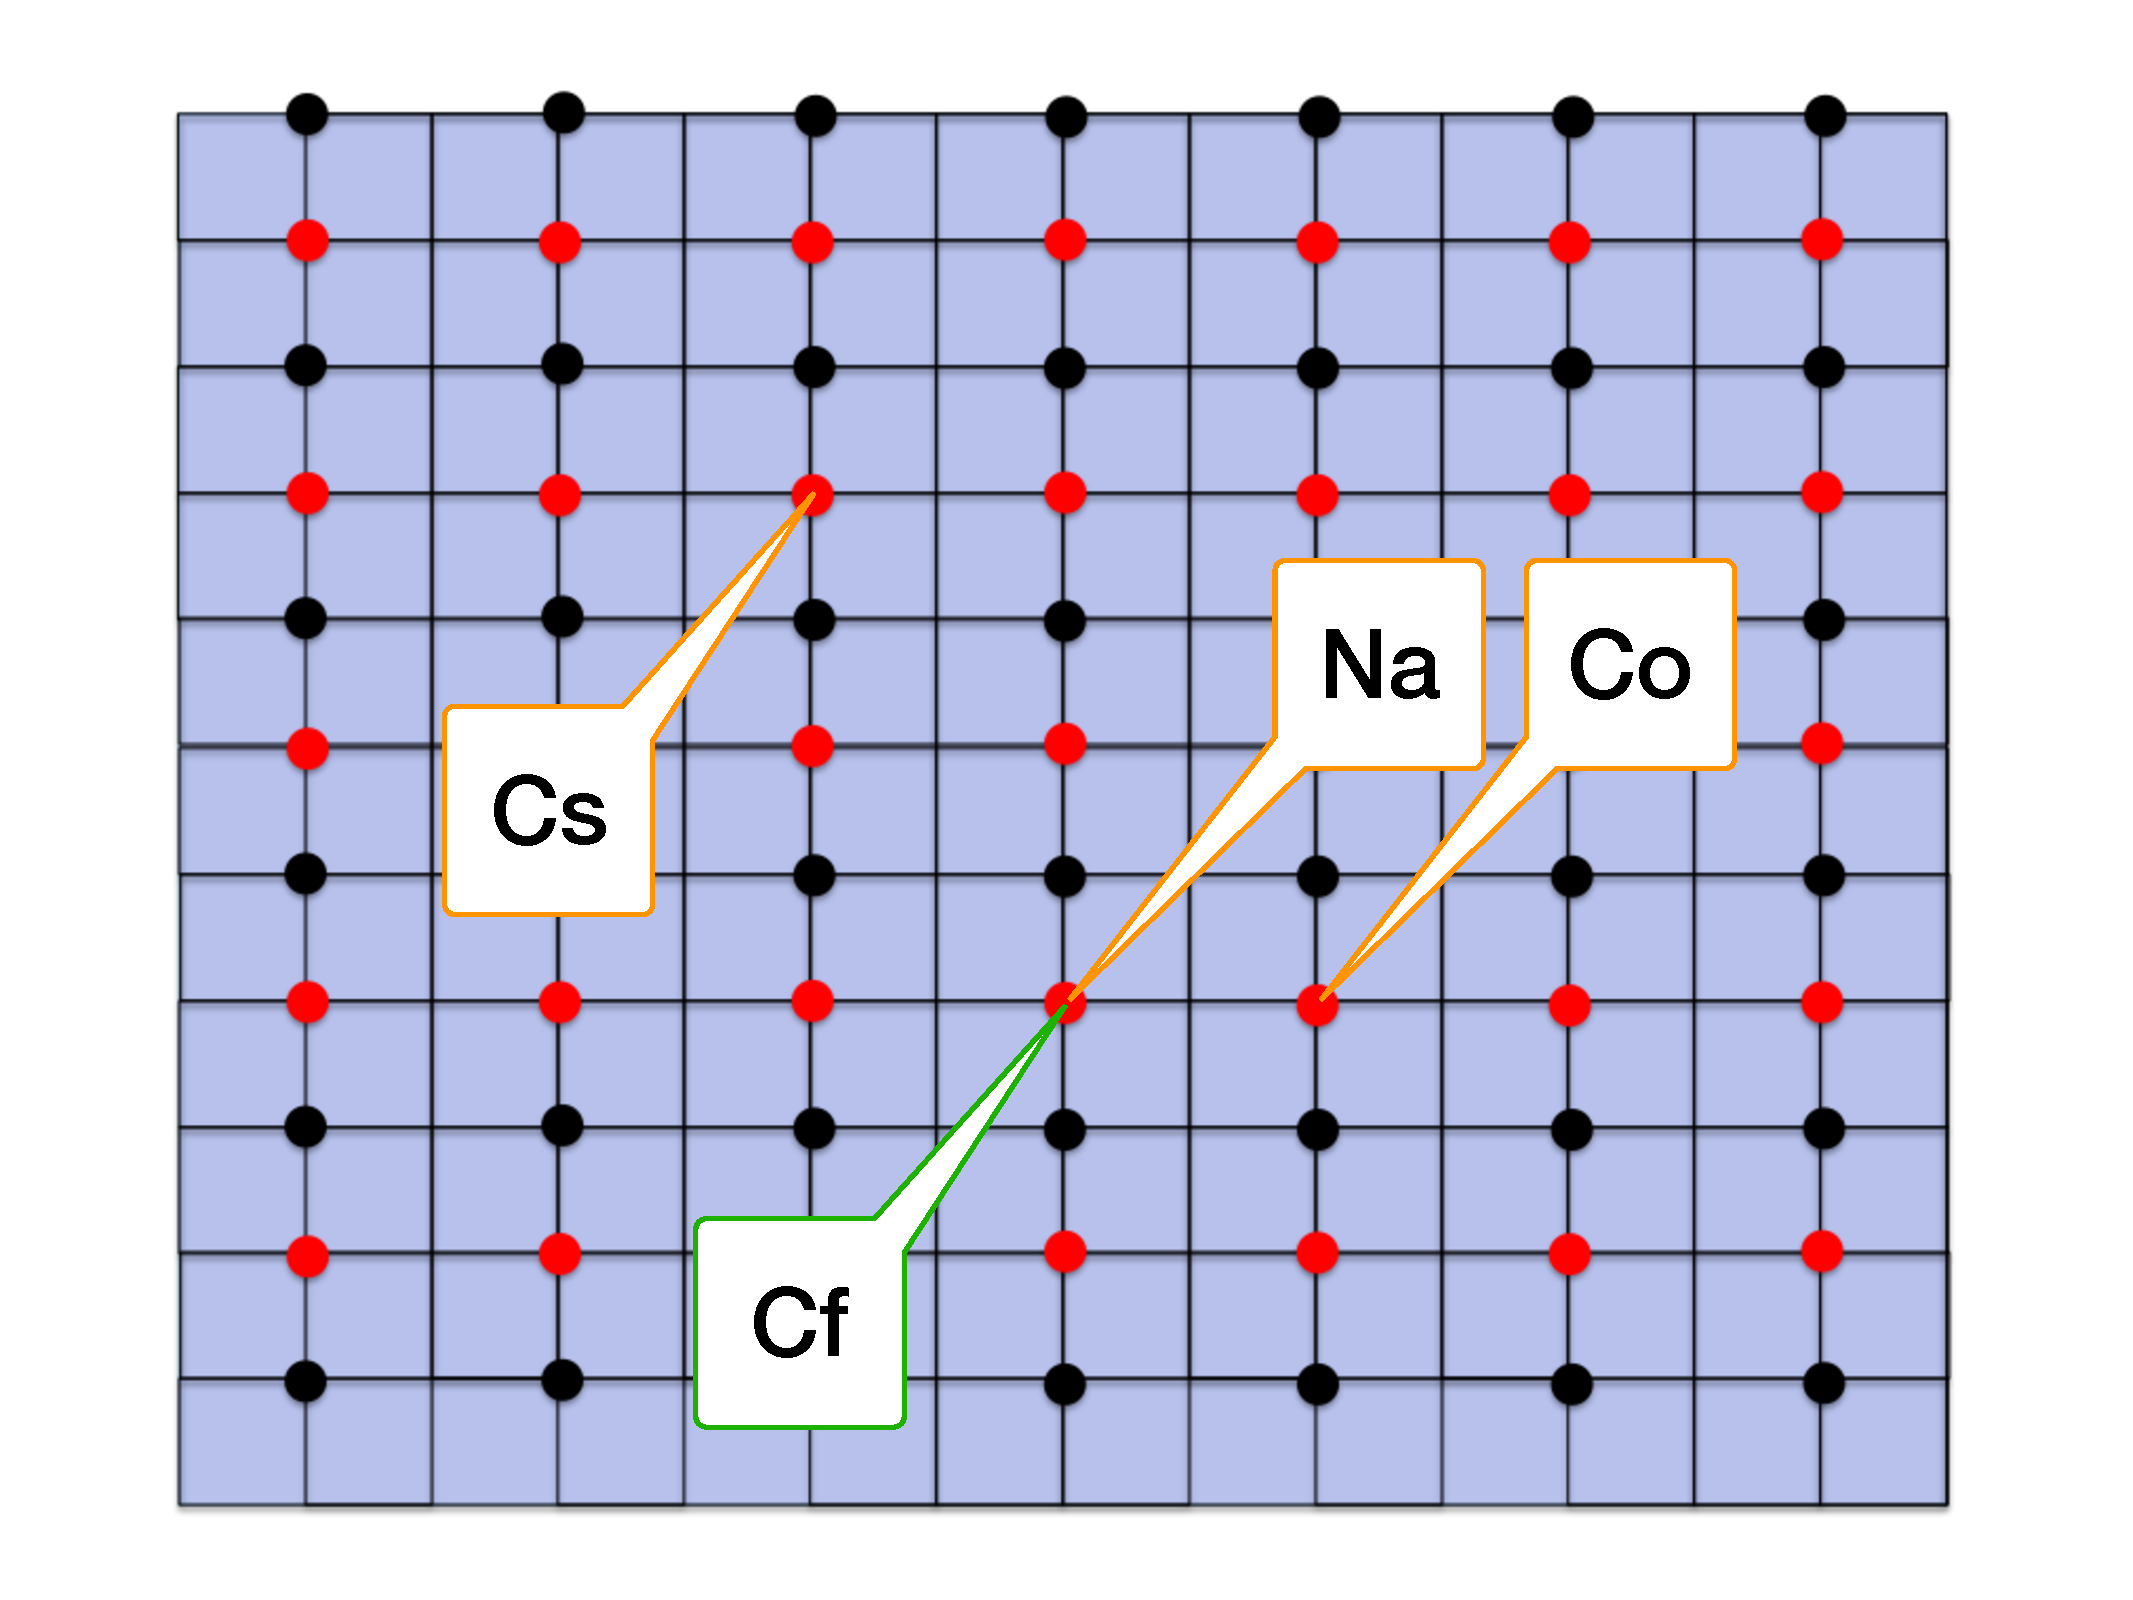
\includegraphics[width=0.6\textwidth]{Figures/CalibMapApril.pdf}\\
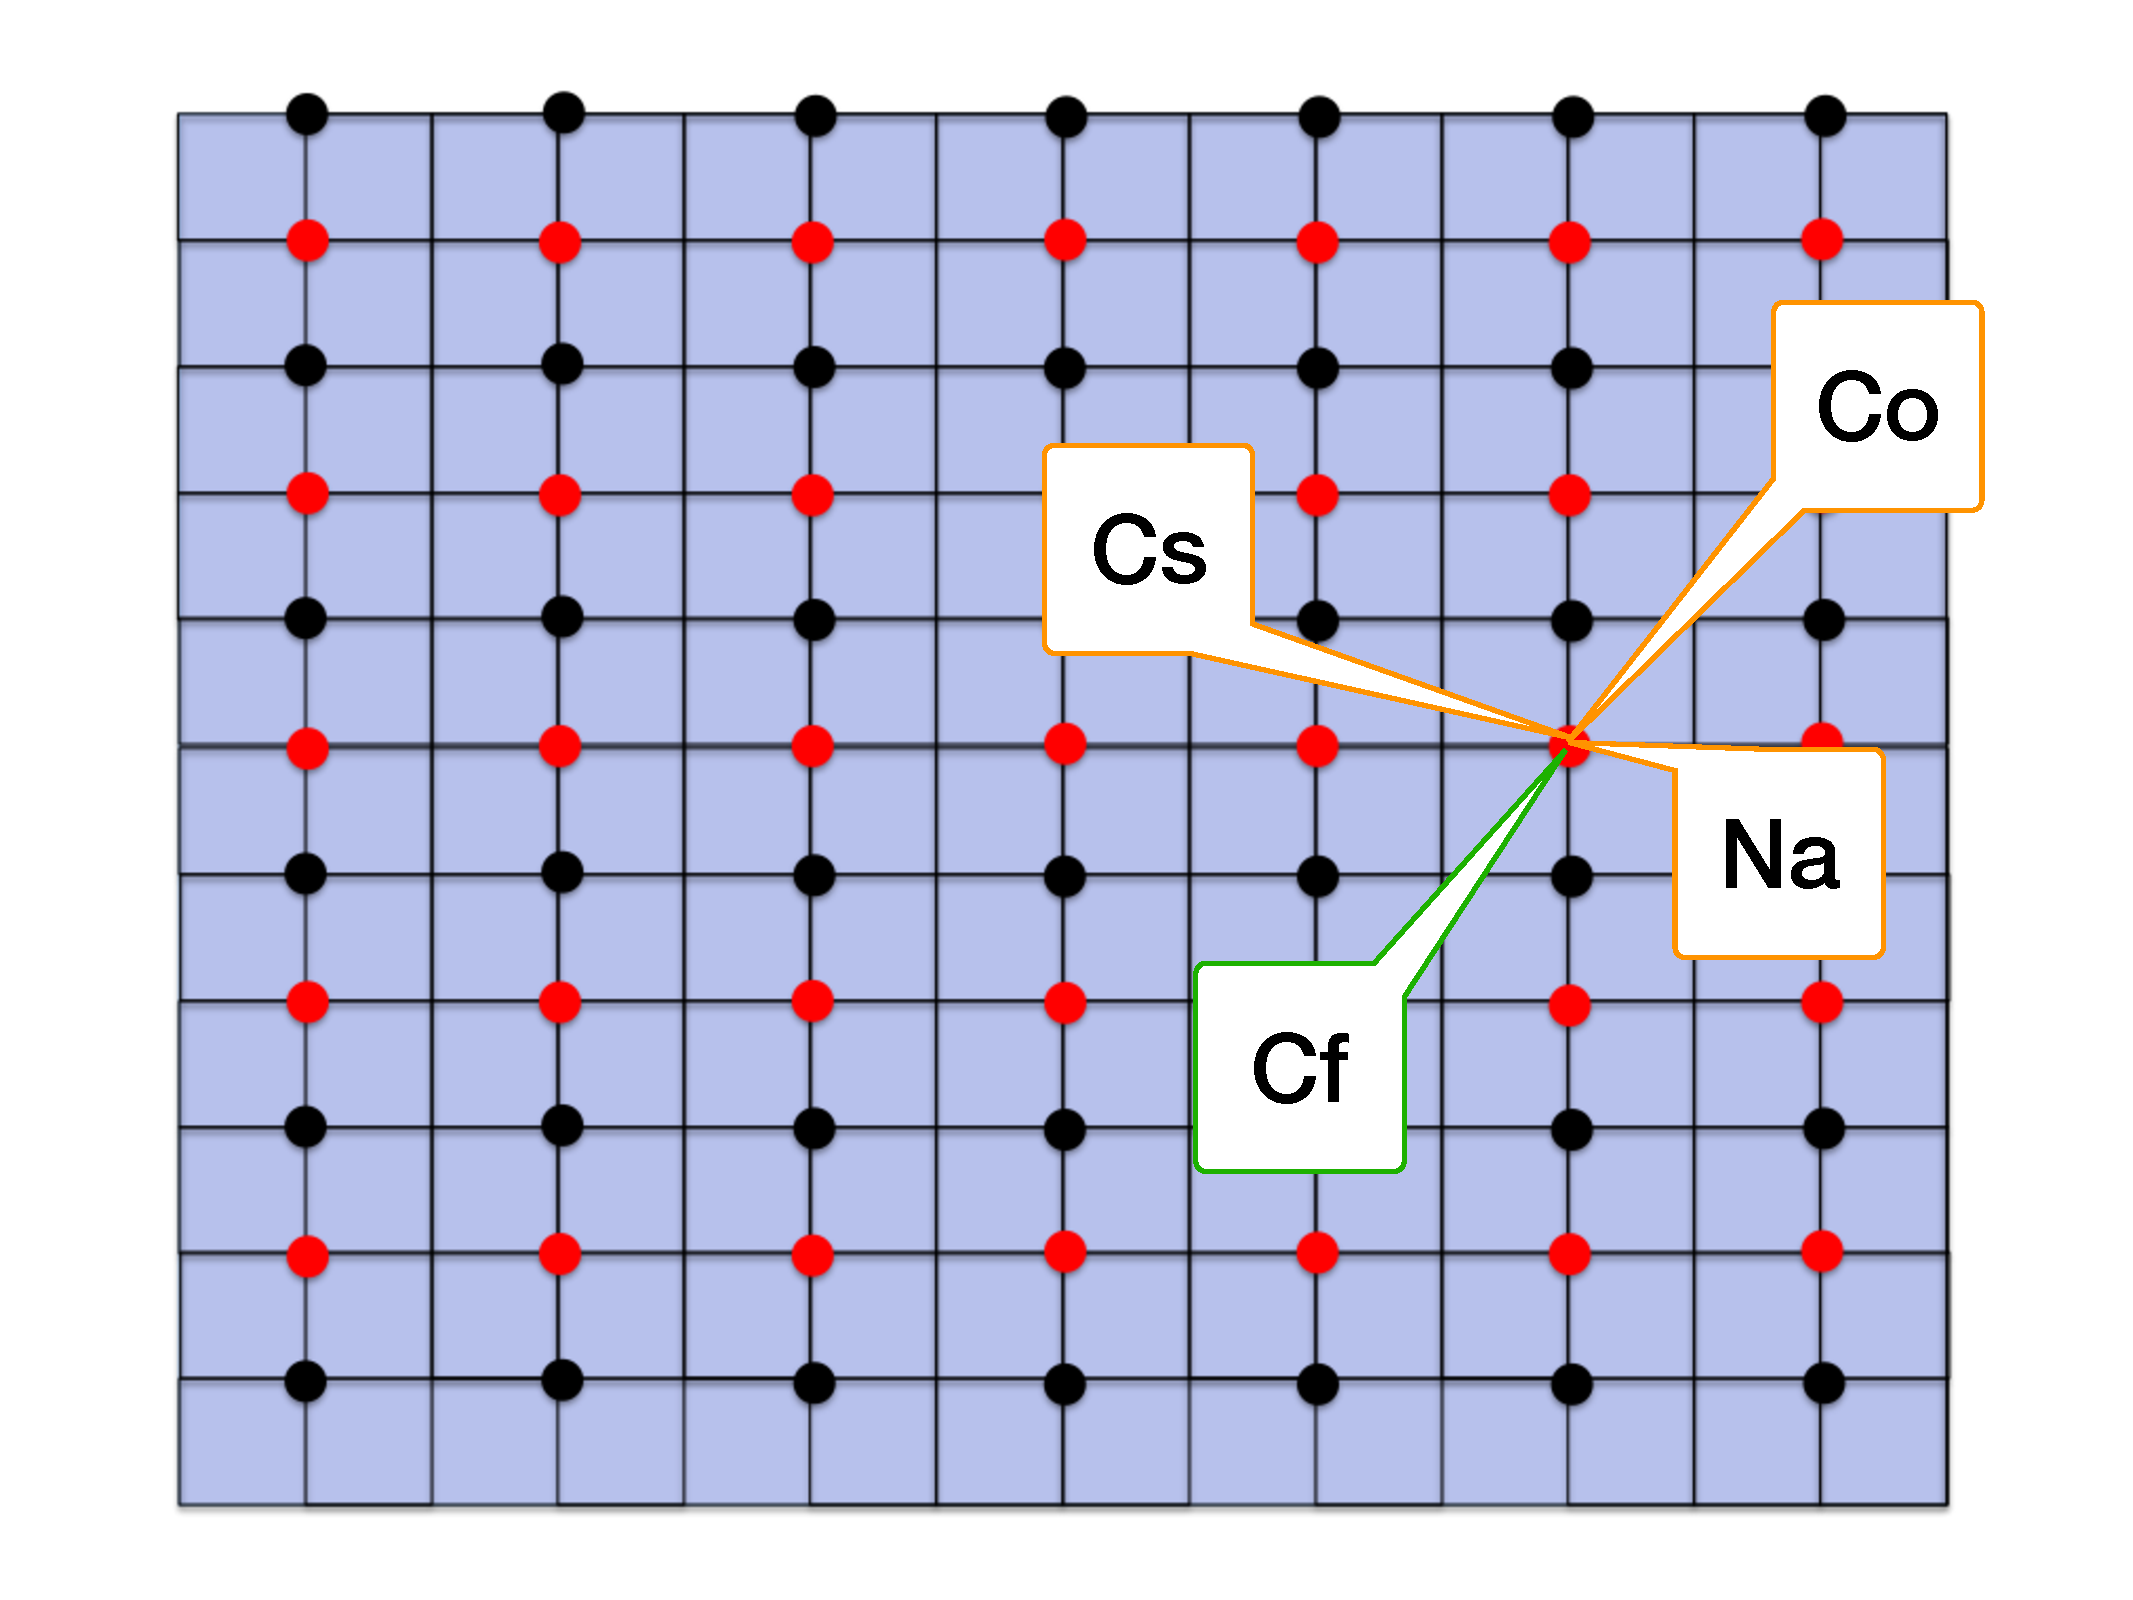
\includegraphics[width=0.6\textwidth]{Figures/CalibMapAug.pdf}\\
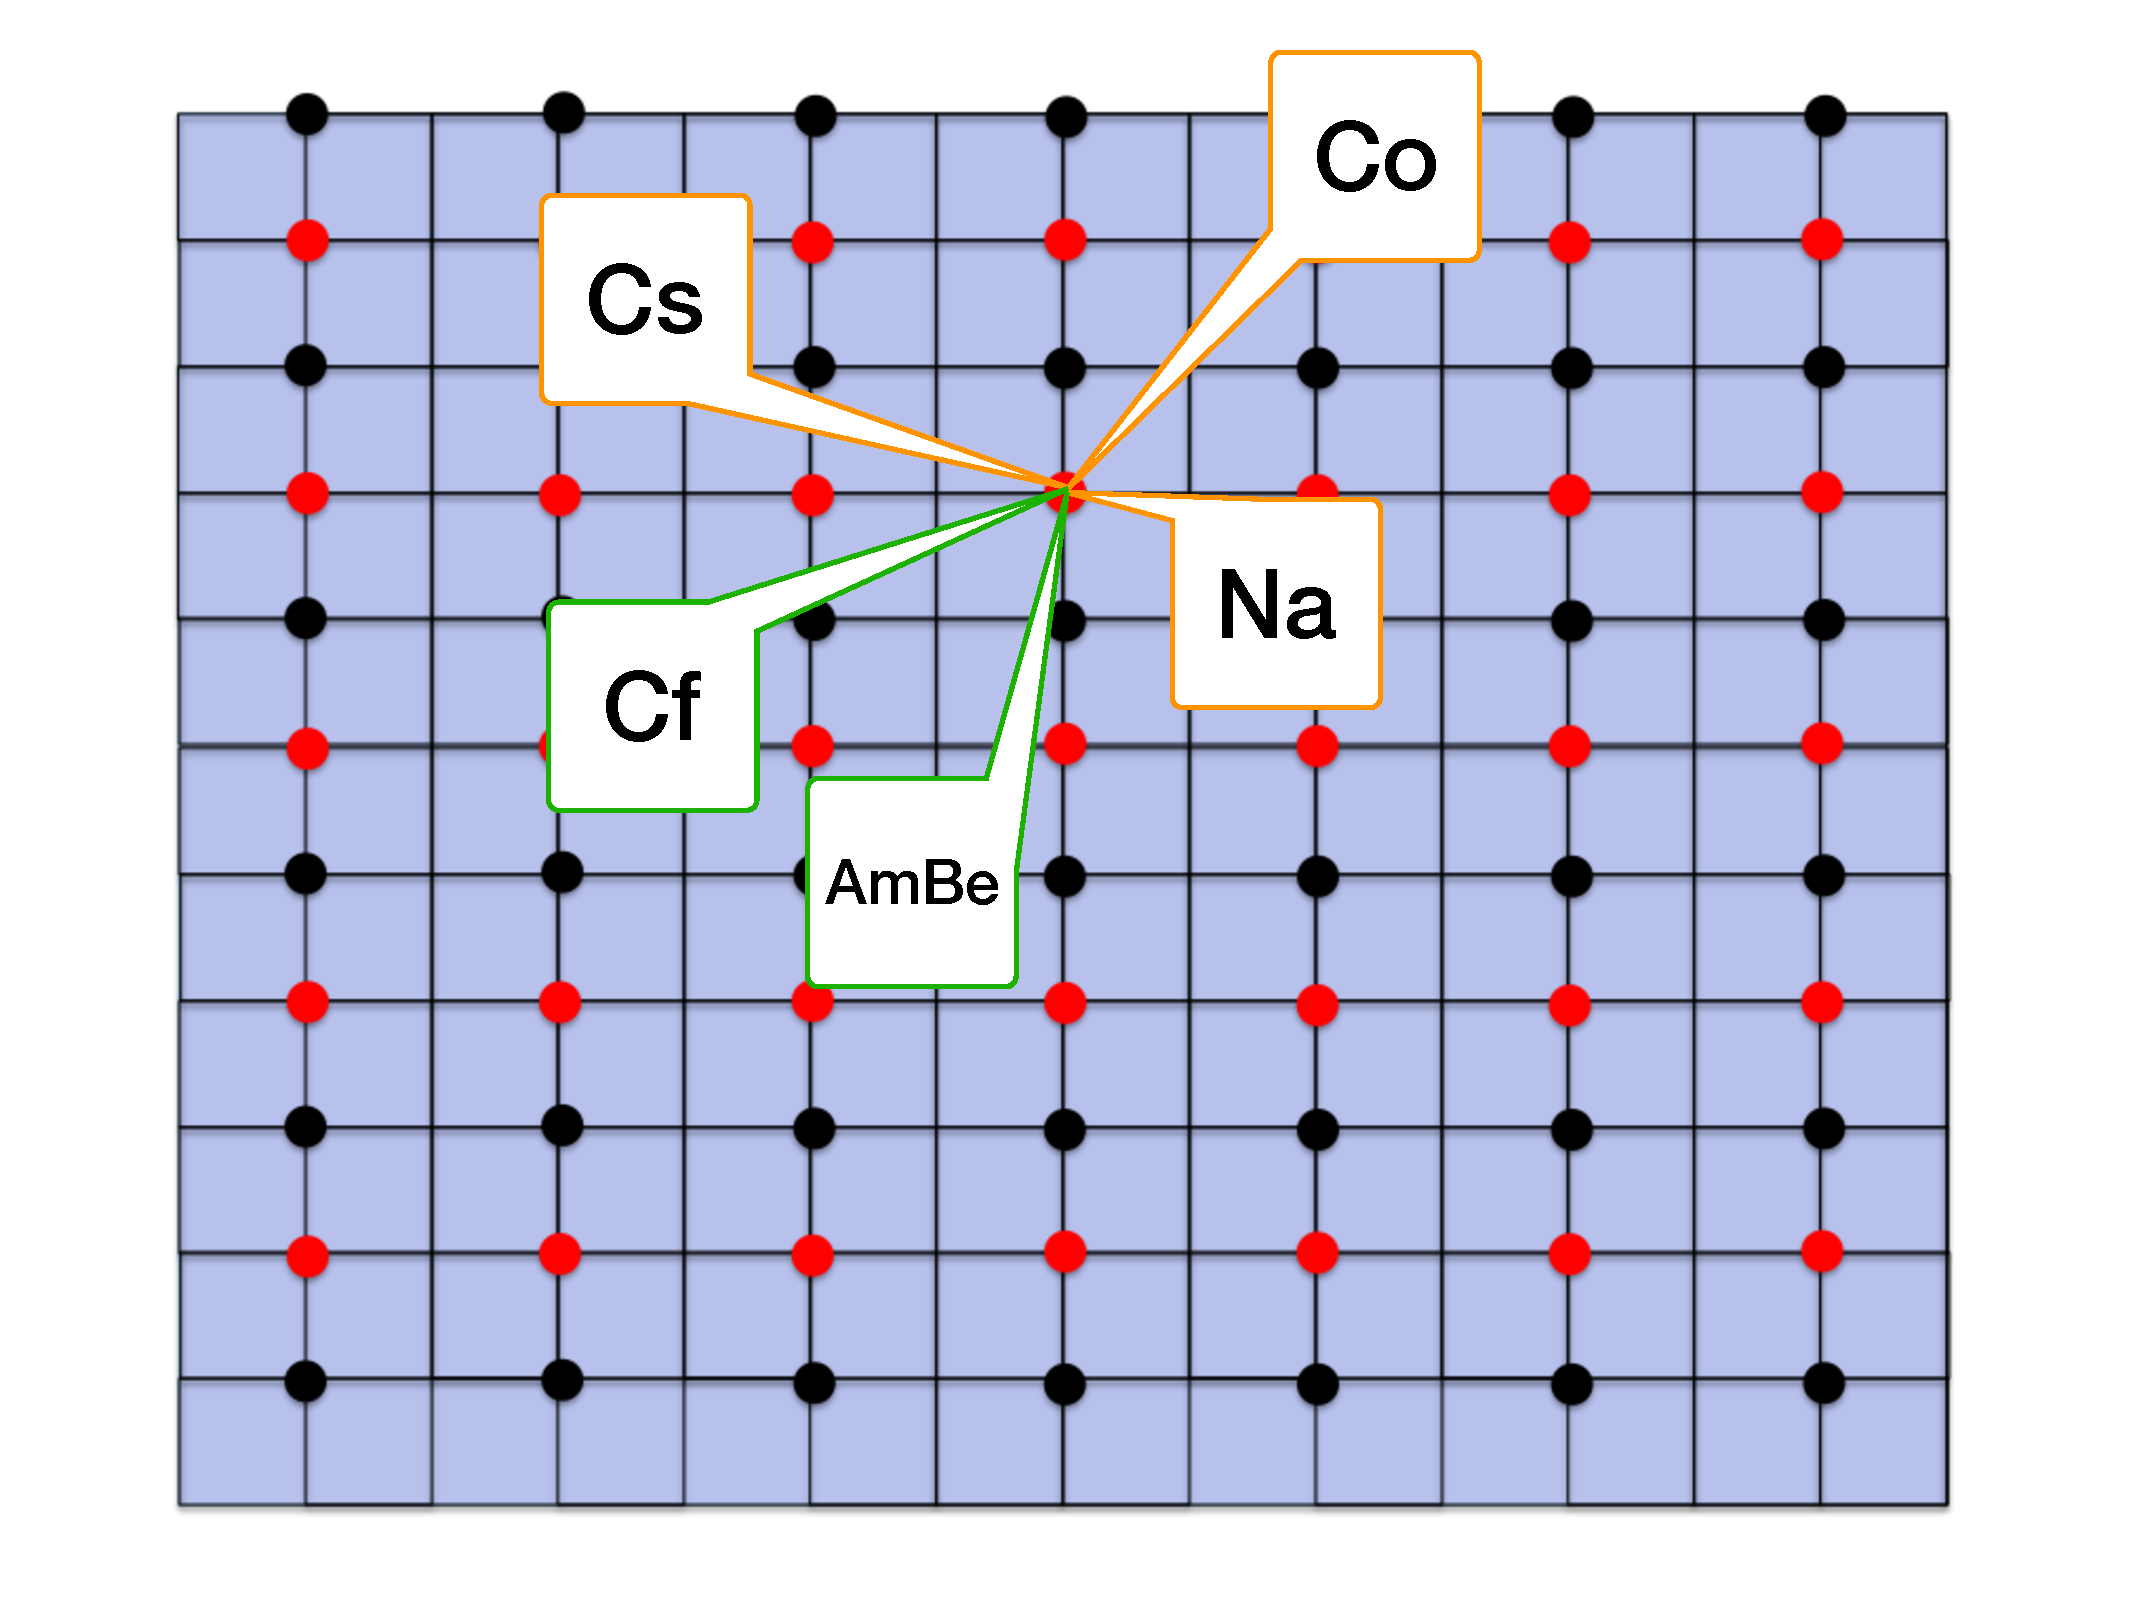
\includegraphics[width=0.6\textwidth]{Figures/CalibMapDec.pdf}
\caption[Positions of the PLA rods used for energy scale calibration runs]{Positions of the PLA rods where specific radioactive source was deployed for energy scale calibrations. 
In this study, each source was deployed at the center of the corresponding PLA rods along $z$-axis.
(Top) Source locations of 2018 April and May calibrations. 
(Middle) Source locations of 2018 August calibrations. 
(Bottom) Source locations of 2018 December calibrations. }
\label{fig:CalibMap}
\end{figure}
\FloatBarrier

During data acquisition, the trigger threshold of each individual PMT channel, referred to as the ZLE thresholds, were set to reduce the electronic noise and low energy backgrounds in collected by each PMT.
The ZLE threshold is a pulse height threshold that requires signal pulses read by PMTs to exceed a specific pulse height.
Only the pulses whose height is above the ZLE threshold are recorded in the DAQ storage.
During gamma and neutron calibrations, the ZLE thresholds were 10 and 20 ADC channels respectively, which is equivalent to 40 to 80~keV.
The light collection varies throughout the PROSPECT AD because of the non-uniformity of the LS attenuation length and light yield efficiency at different positions in the detector.
In addition, PMT gain and scintillation light yield of PROSPECT AD also dependent on time in PROSPECT AD.
Thus, the ZLE threshold can induce non-uniform reconstructed energy scale based on the position and time of the incident particle.
A 90~keV detector-wide `analysis ZLE threshold' is introduced to exclude segment hits whose reconstructed energies are lower than 90~keV.
This analysis ZLE threshold resolves the non-uniformity of lower energy reconstruction that is caused by the time and position dependent event selection efficiency.
To unpack and analyze the calibration data, the PROSPECT-2x (P2x) analysis package is used to reconstruct the gamma energy of clusters in the full detector and the Compton scattering energy deposited in single segments. 
Once again, the reconstructed energy is the summed energy of all hits in an cluster that passed the analysis ZLE threshold.

The reconstructed energy resolution is highly dependent on the photostatistics of events. 
Therefore, the energy resolution varies with respect to the non-uniformity of light collection among segments and evolve during the data acquisition period.
In data unpacking and analysis, each hit of a cluster is artificially smeared based on the lowest photostatistics dataset in the sample, 325~PE/MeV, as shown in Figure~\ref{fig:PEvTime}.

\begin{figure}[h!]
\centering
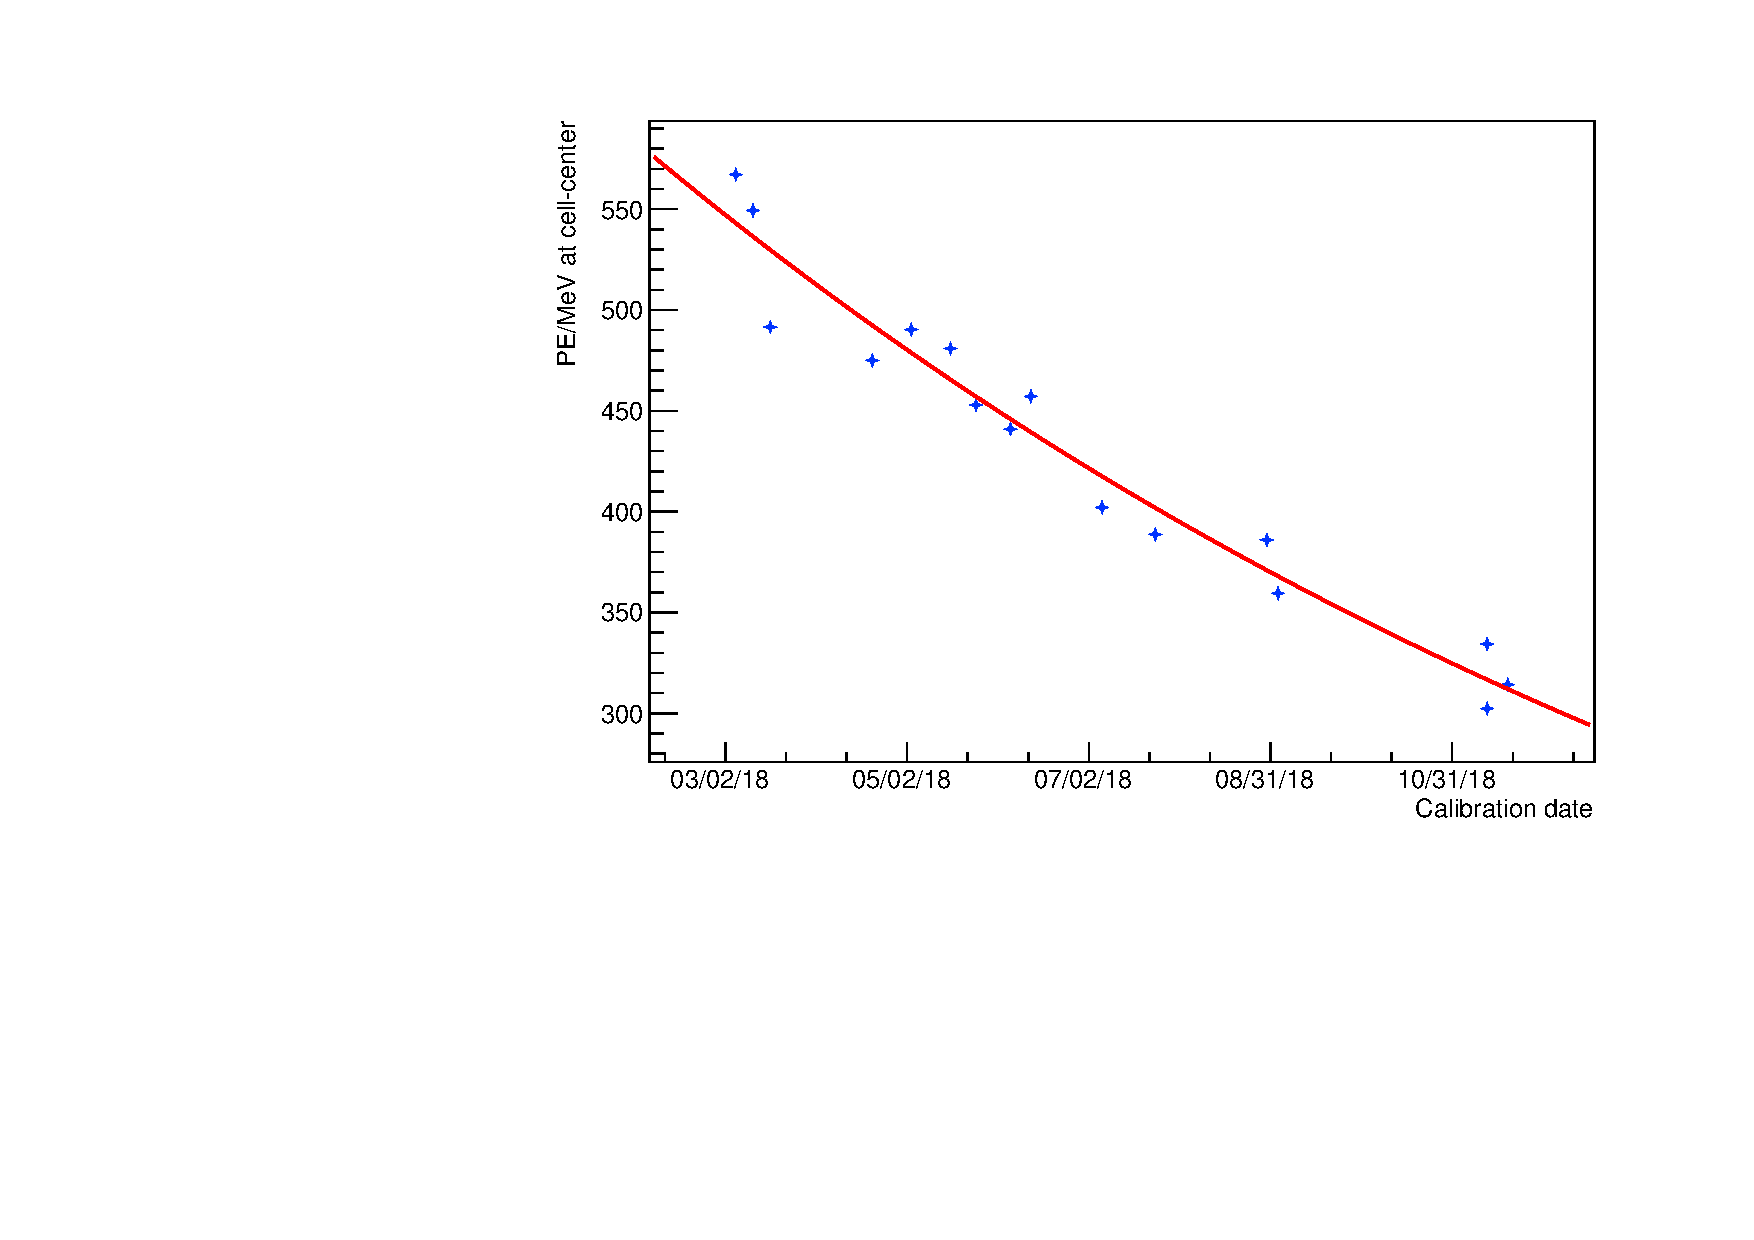
\includegraphics[width=0.7\textwidth]{Figures/PEvsTime.pdf}
\caption[The PE per MeV evolution over time]{PE per MeV tracked through the total data acquisition period. The fitted function suggests 346$\pm$17 PE/MeV at the end of the period.}
\label{fig:PEvTime}
\end{figure}

The reconstructed energy of each event is smeared based on the calibrated effective PE/MeV factor characterized with cosmogenic neutrons captured by $^6$Li in each run. 
Every hit is smeared with a factor randomly chosen from a Gaussian distribution, whose standard deviation is defined as
\begin{equation}
	\sigma = E\cdot\sqrt{\frac{1}{k} - \frac{1}{n}},
\end{equation}
where $k$ is the target PE/MeV factor and $n$ is the measured PE/MeV factor.

In a summary, an event energy is reconstructed with an additional threshold and randomized resolution correction.
The purpose of these two additional adjustments is to eliminate the energy scale and resolution's dependence on events' time and position.

\Section{Calibration Event Reconstruction}

For gamma source calibration, $^{137}$Cs, $^{22}$Na and $^{60}$Co sources were deployed.
The gamma-like events are selected within the 3$\sigma$ range of the mean PSD value for gammas and electrons.
Background events were analyzed with the background data described in Section~\ref{sec:calibration}.
The selection of background events is identical to the selection gamma calibration event.

The time coincidence between prompt and delayed $\gamma$-rays is searched to select the $n$-H capture gamma energy.
The prompt $\gamma$-rays (3 MeV to 15 MeV) are emitted from the $^{252}$Cf fission reaction, while the delayed $\gamma$ ray is the 2.22~MeV de-excitation $\gamma$ from the $n$-H capture interaction.
Using PSD distribution bands, $\gamma$-ray-like events within 0 to 200 \textmu s after the prompt $\gamma$ signal were tagged as $^{252}$Cf correlated $\gamma$ events, while the events -1200 to -200 \textmu s before prompt $\gamma$ are accidental.
The $n$-H $\gamma$ spectrum is measured by subtracting the correlated events in background data.
The calibration spectra is shown in Figure \ref{fig:gammacalib}.

\begin{figure}[!ht]
\centering
\subfigure[]{\label{fig:caliba}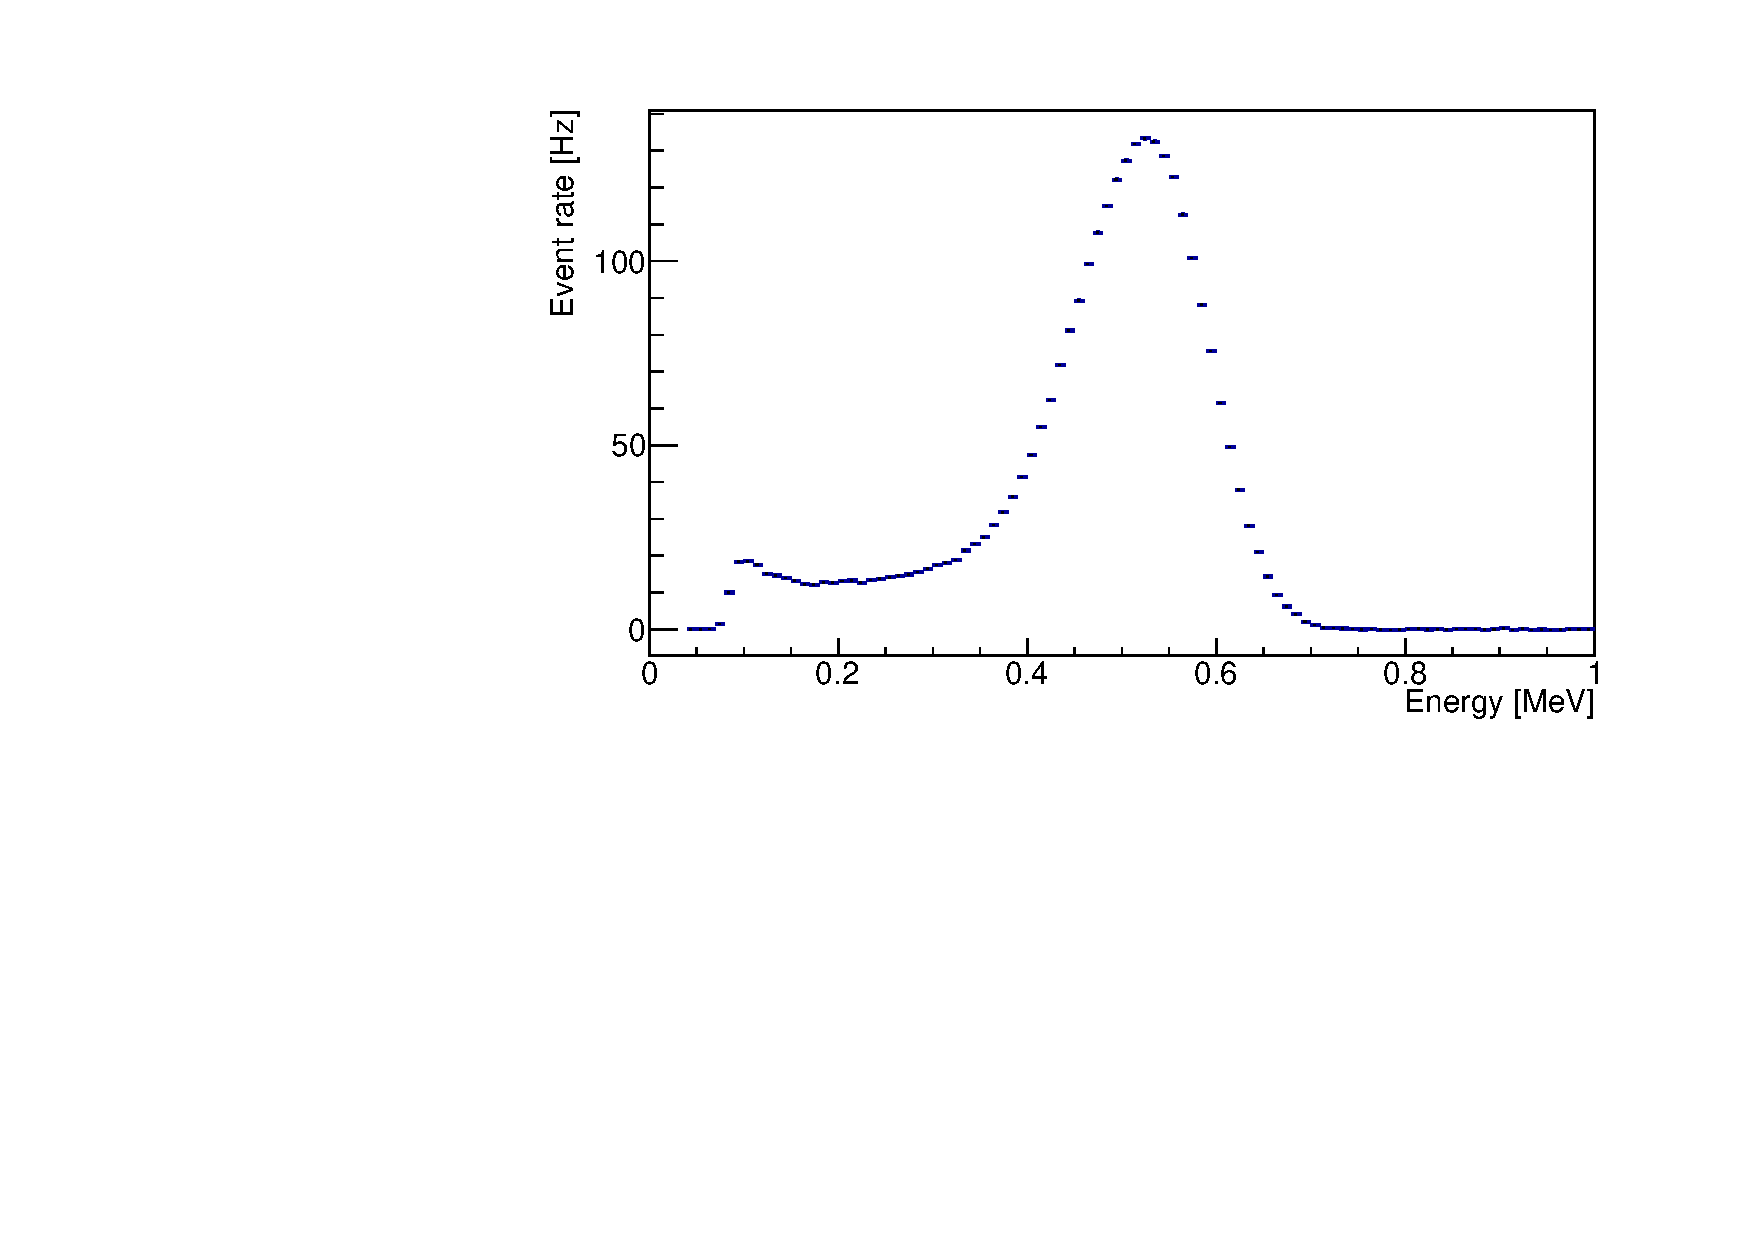
\includegraphics[width=65mm]{Figures/Cs137smear85.pdf}}\quad
\subfigure[]{\label{fig:calibb}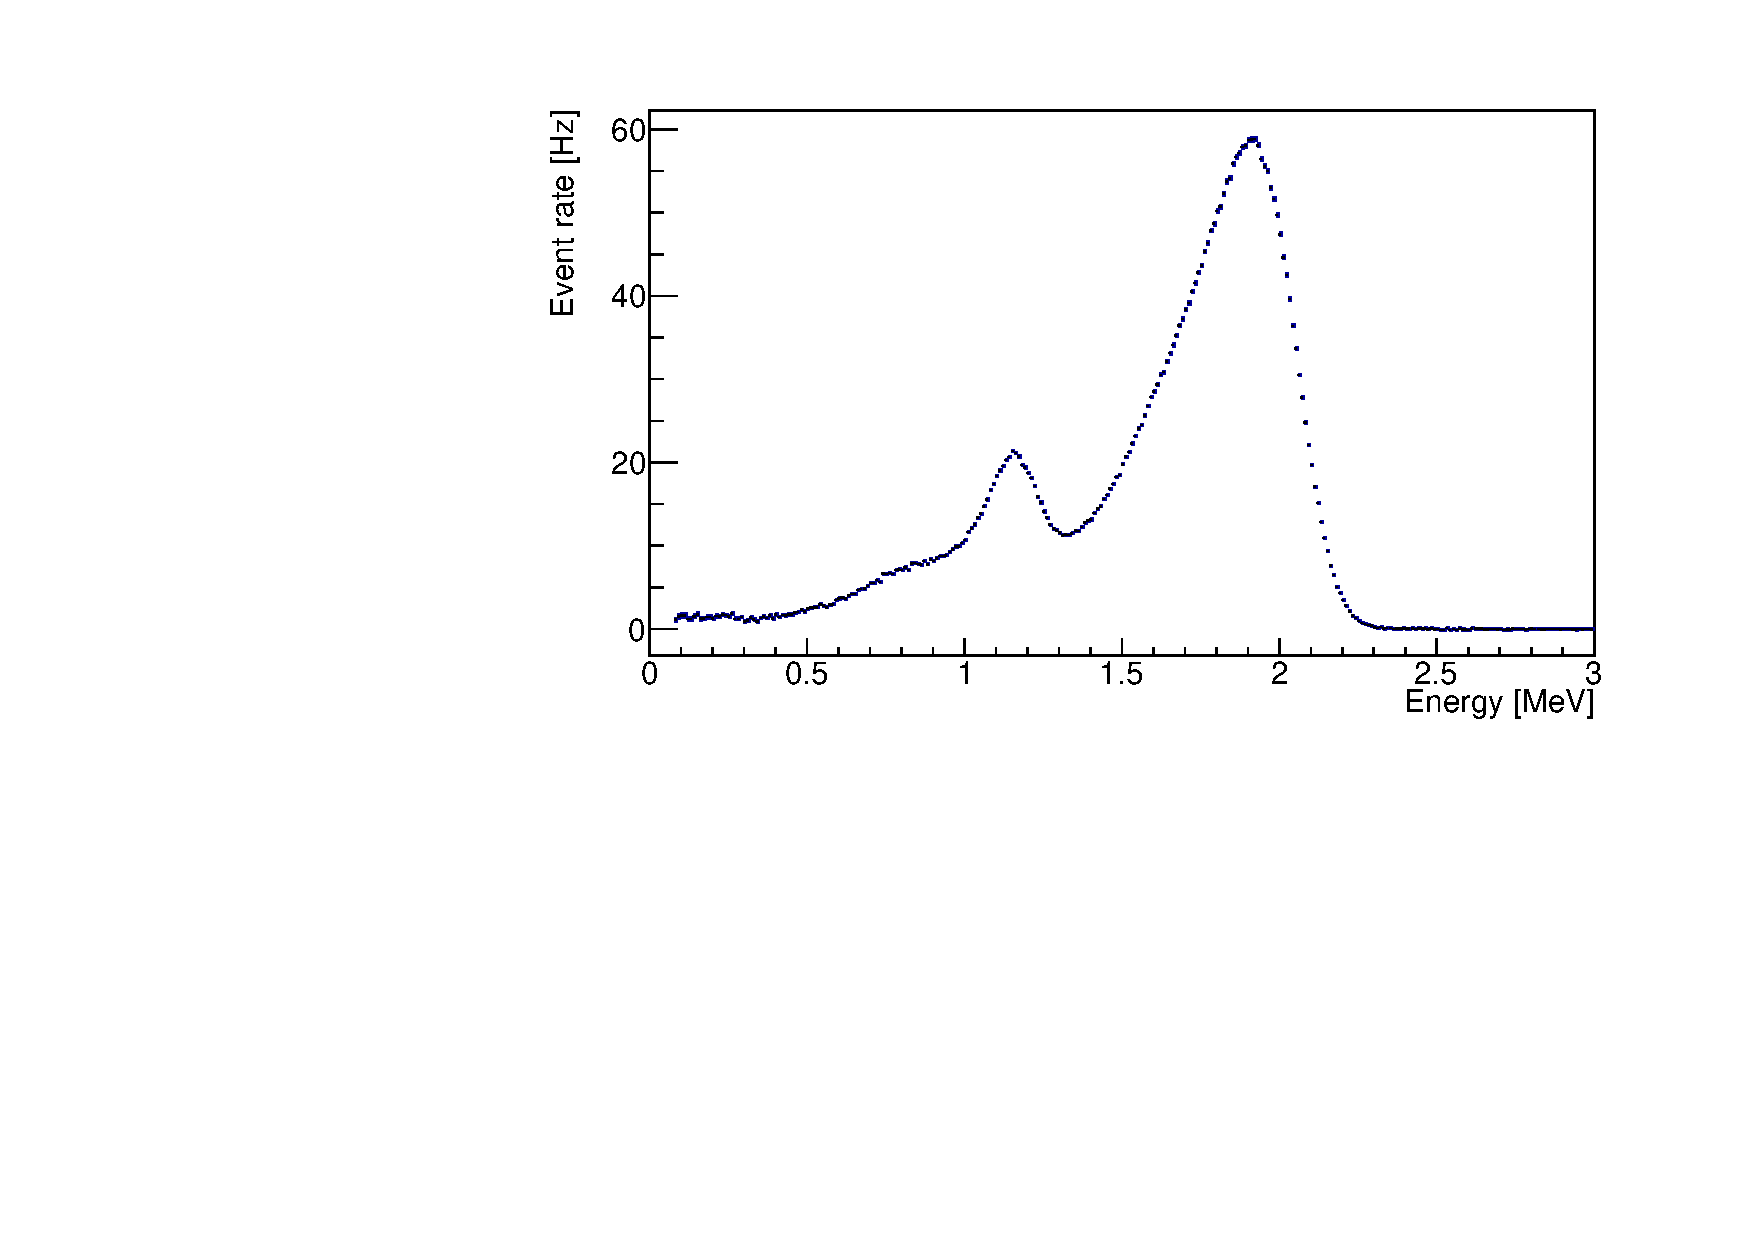
\includegraphics[width=65mm]{Figures/Na22smear85.pdf}} \\
\subfigure[]{\label{fig:calibc}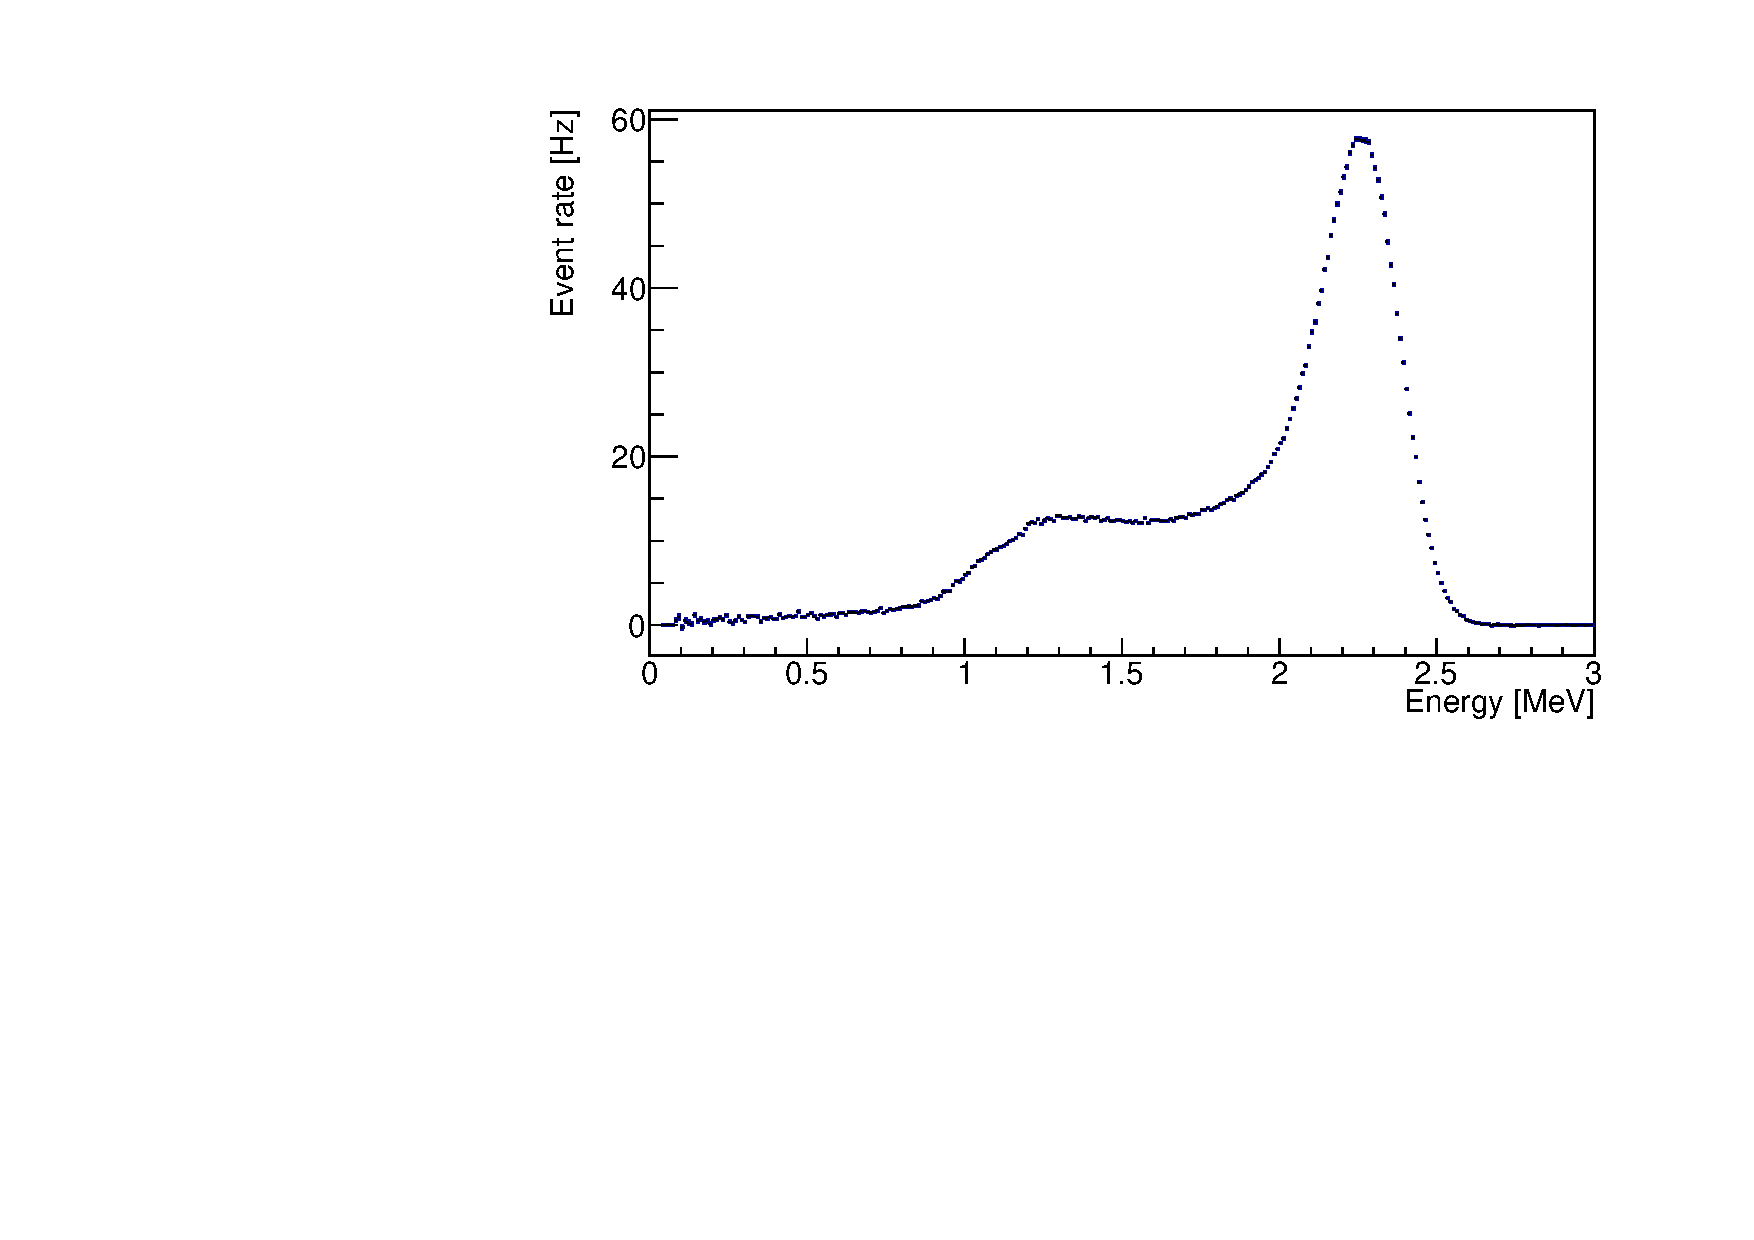
\includegraphics[width=65mm]{Figures/Co60smear85.pdf}} 
\subfigure[]{\label{fig:calibd}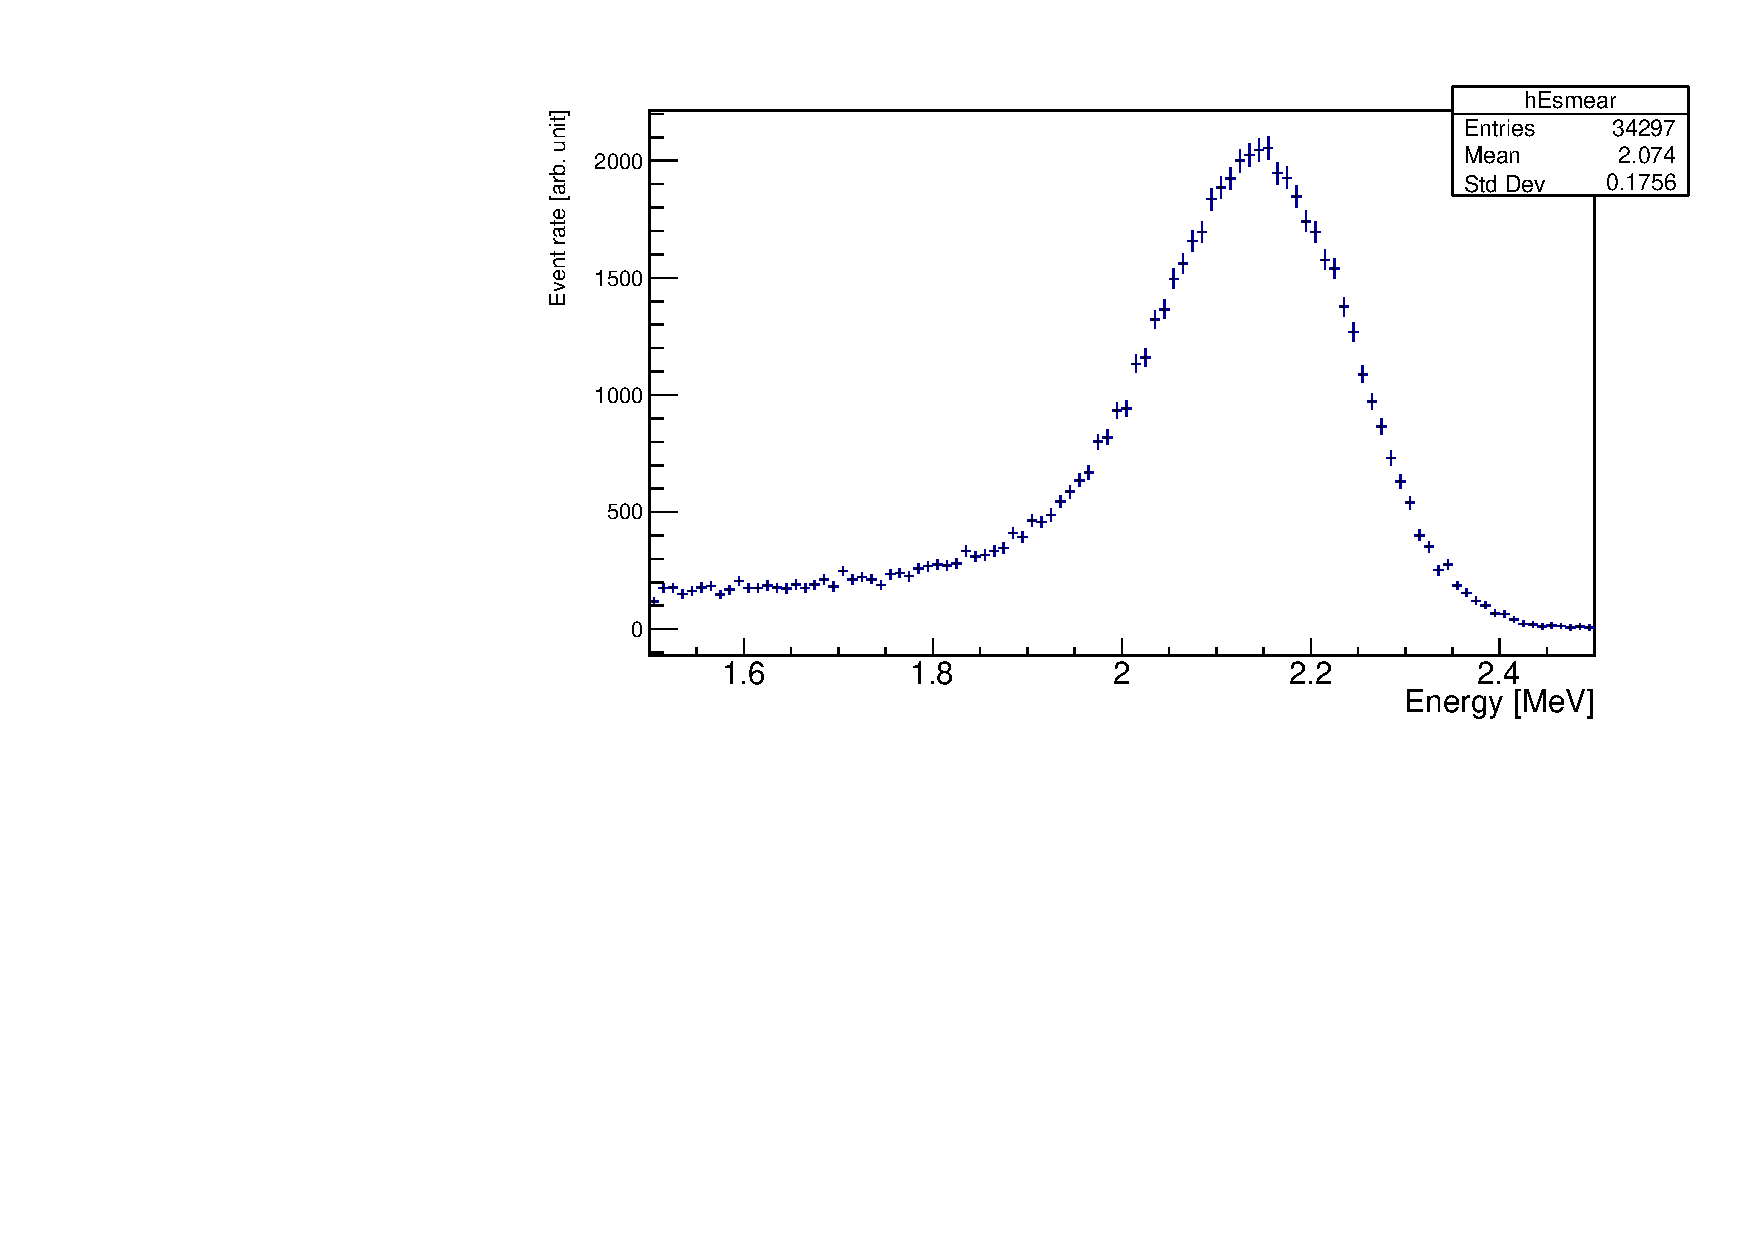
\includegraphics[width=65mm]{Figures/Cf252smear85.pdf}}
\caption[Calibration gamma spectra reconstructed with the full PROSPECT AD]{
The gamma spectra reconstructed with the full PROSPECT AD from calibration sources: (a) $^{137}$Cs, (b) $^{22}$Na, (c) $^{60}$Co, (d) $n$-H capture gamma from $^{252}$Cf.
}
\label{fig:gammacalib}
\end{figure}

The number of gammas generated by the decay of each calibration source, as well as the energy of each produced gamma ray are different. 
As a result, different gamma calibration source generate $\gamma$-rays that deposit energy in different number of segments.
The number of segments hit by a cluster (multiplicity) in the full PROSPECT detector is a critical variable that affects the reconstructed energy, because of its correlation with the energy loss caused by the dead volume and segment a particle traveled through.
The multiplicity of the calibration gamma rays are shown in Figure~\ref{fig:gammamulti}.
The correlation between a cluster's multiplicity and energy is detailed in Section~\ref{sec:dataMC}.

\begin{figure}[!ht]
\centering
\subfigure[]{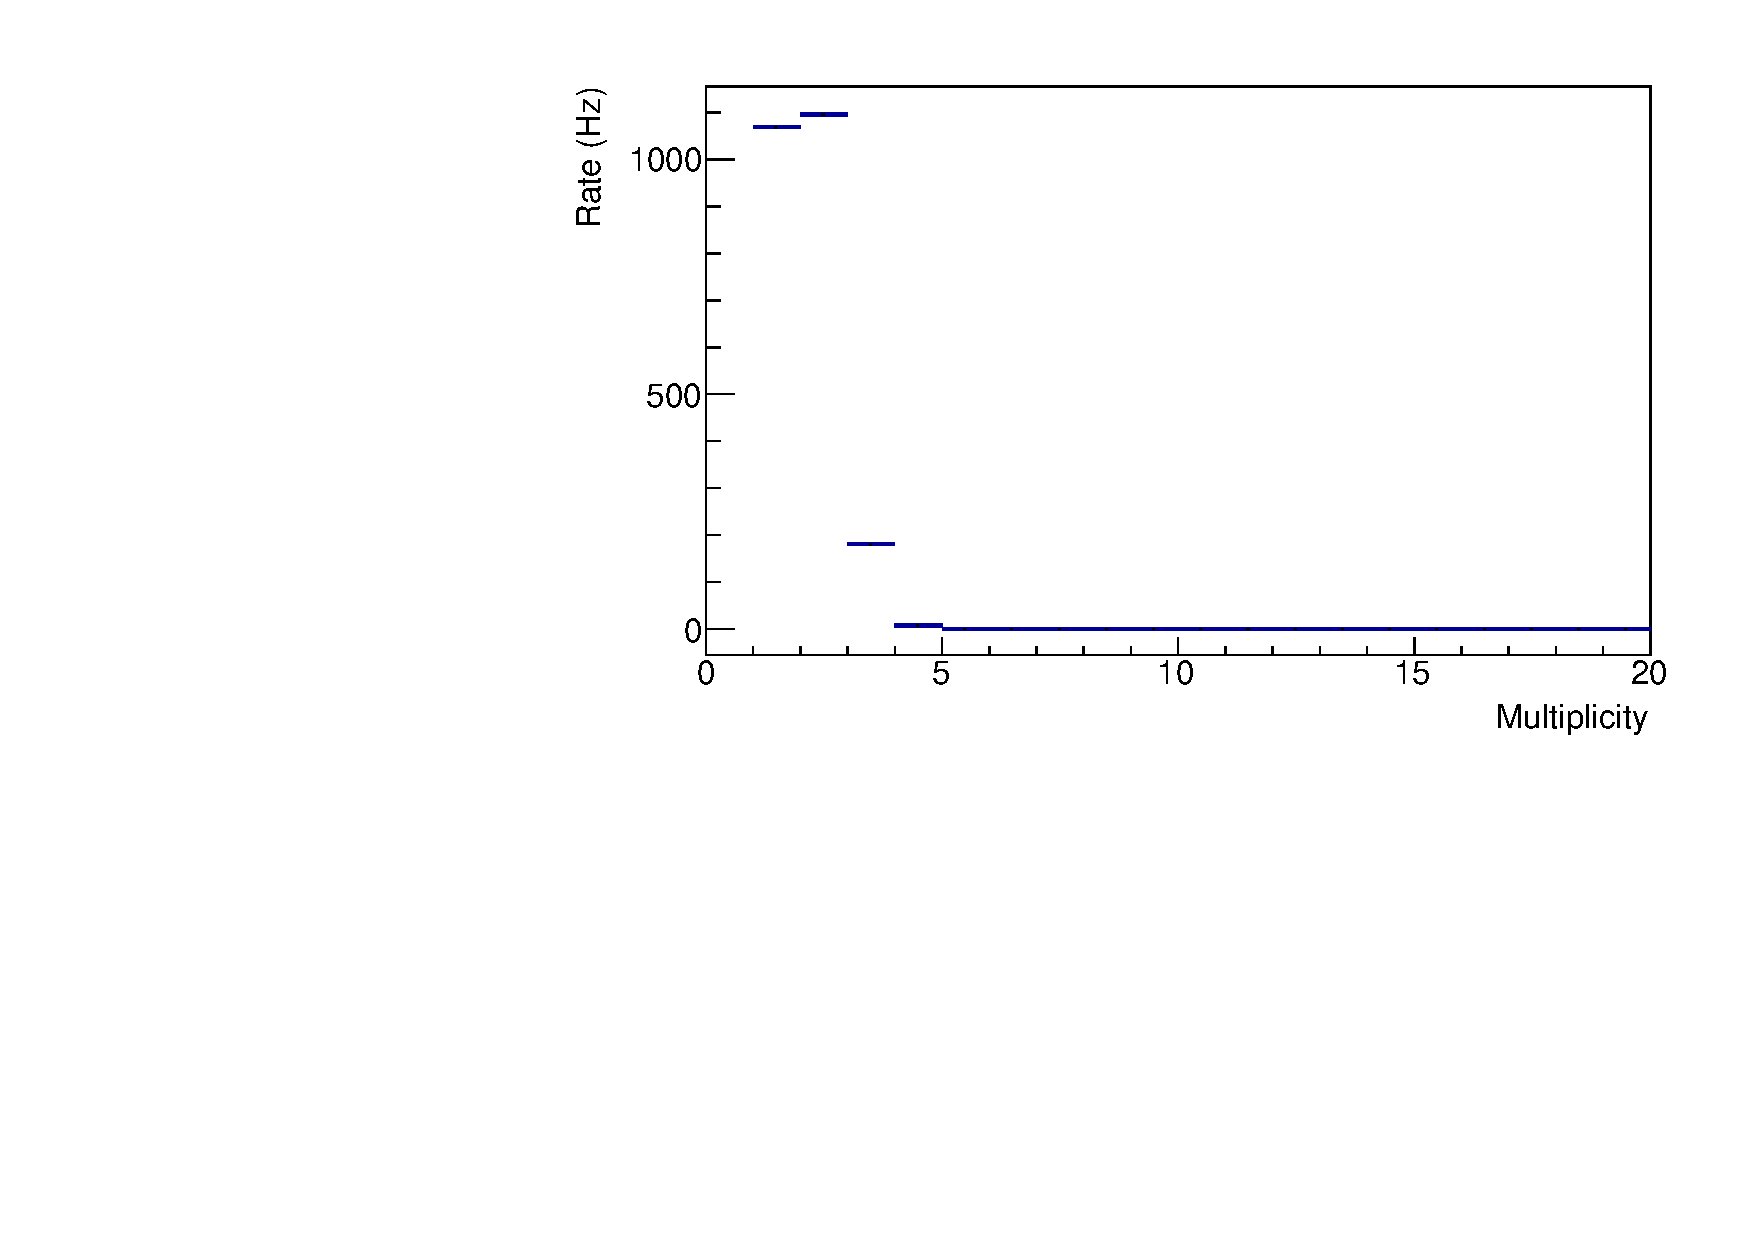
\includegraphics[width=65mm]{Figures/Cs137Multi.pdf}}\quad
\subfigure[]{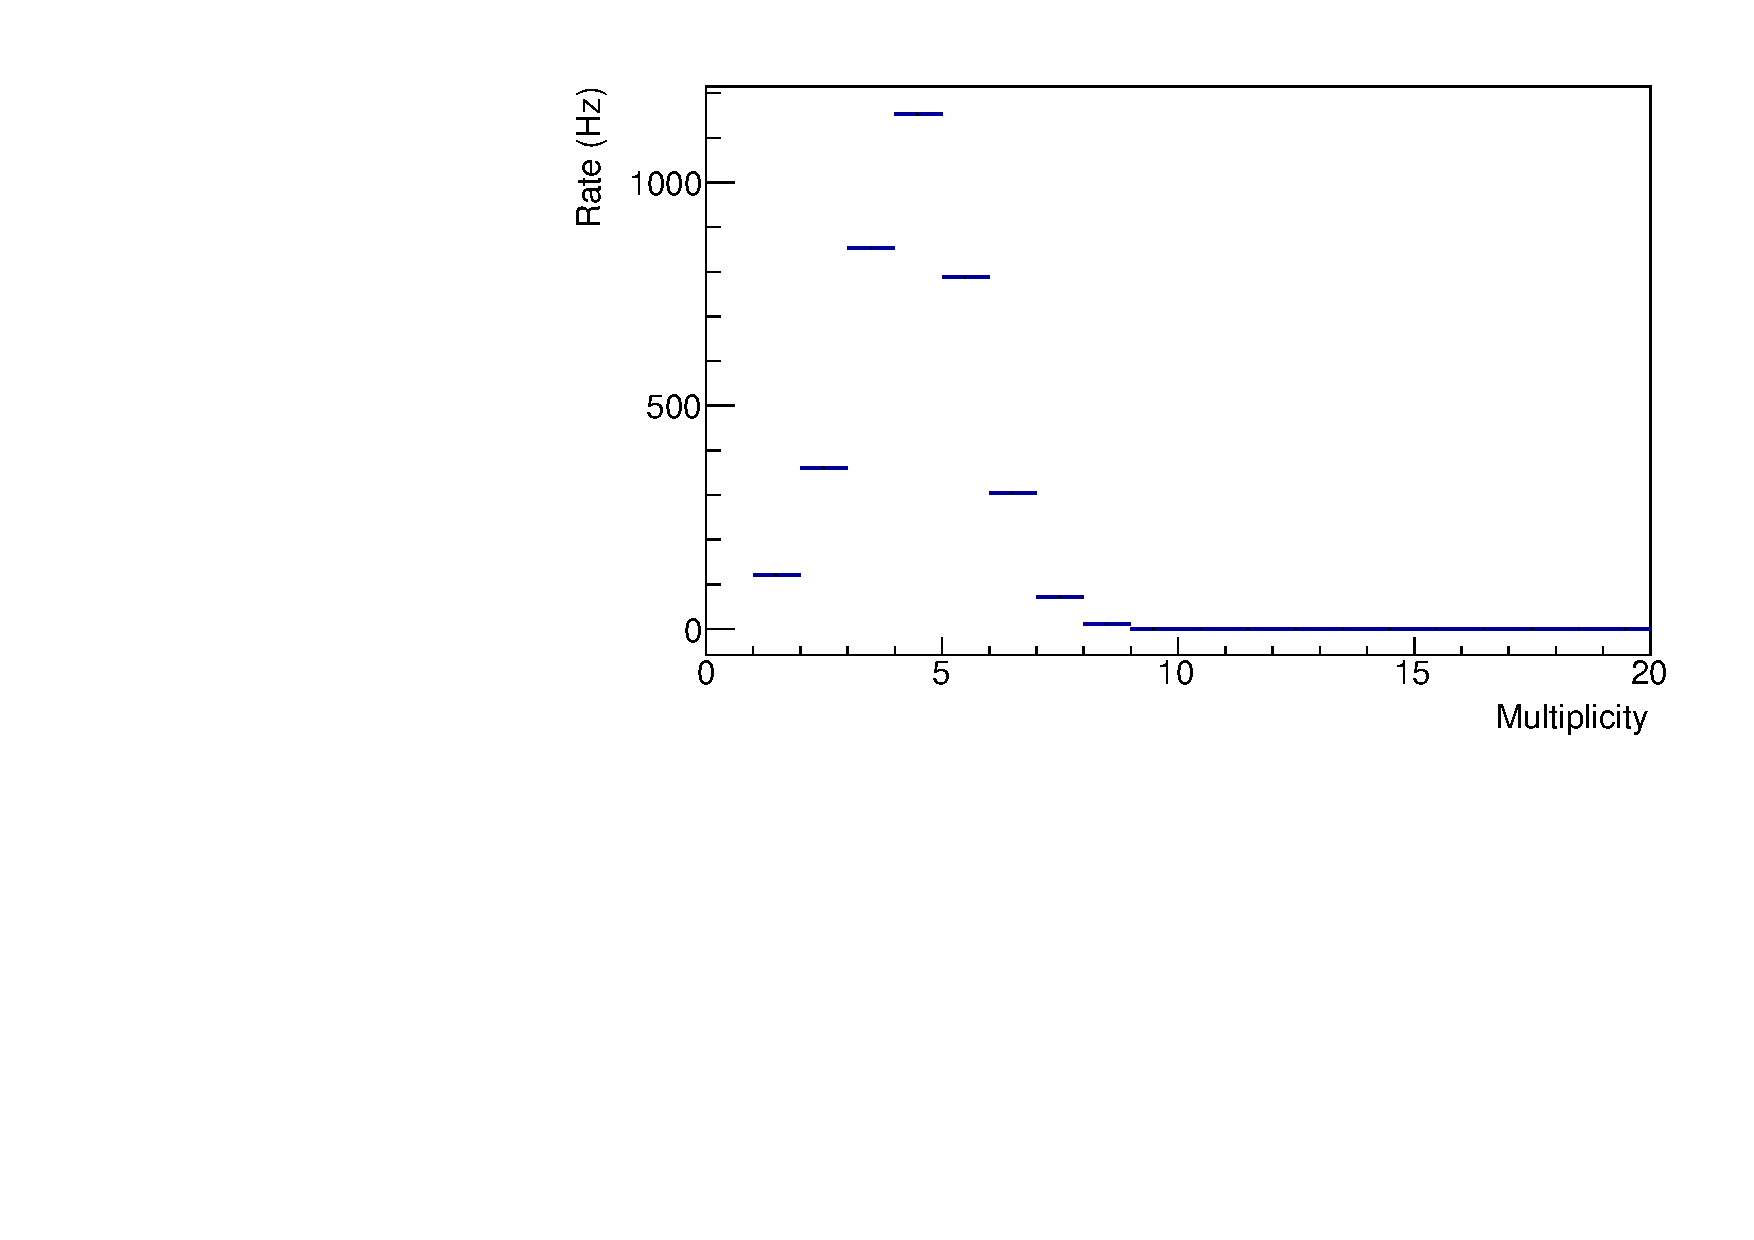
\includegraphics[width=65mm]{Figures/Na22Multi.pdf}} \\
\subfigure[]{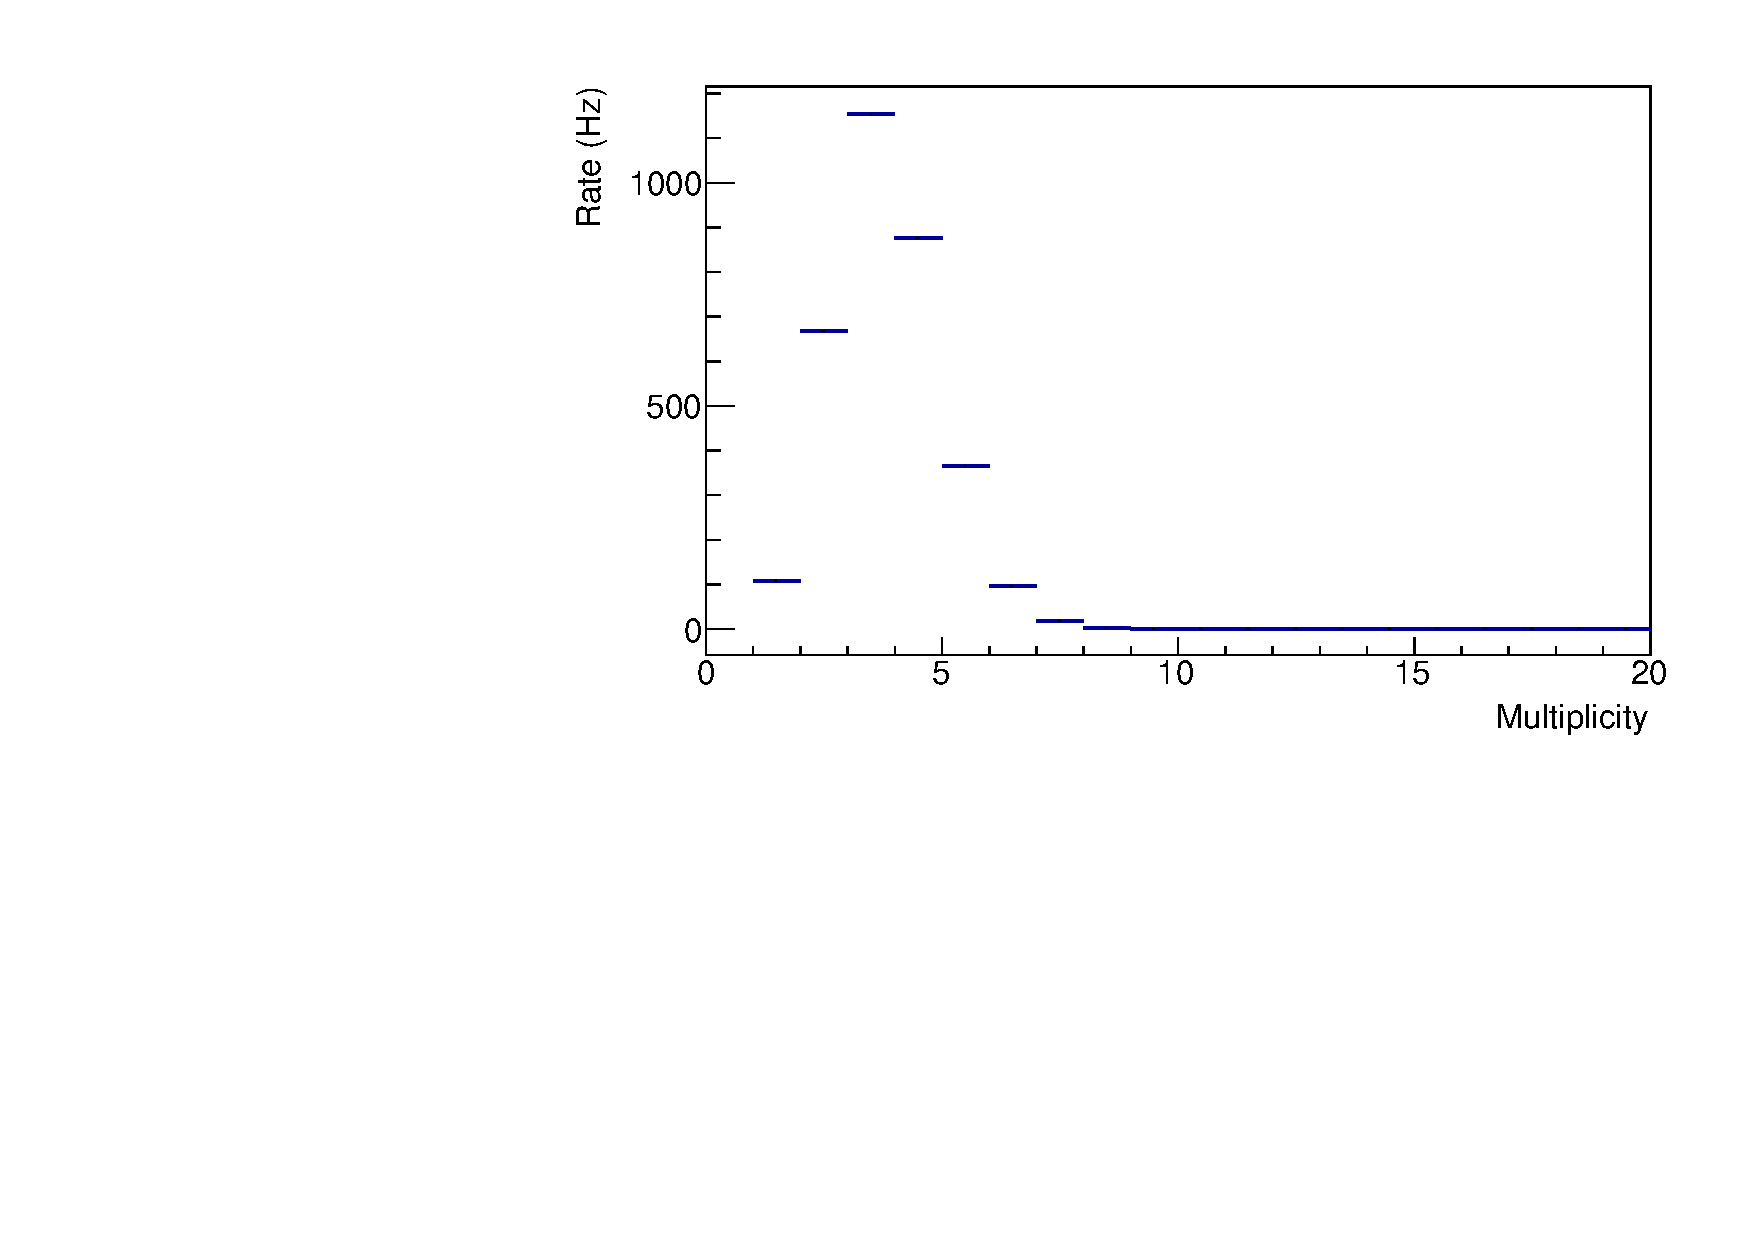
\includegraphics[width=65mm]{Figures/Co60Multi.pdf}} 
\subfigure[]{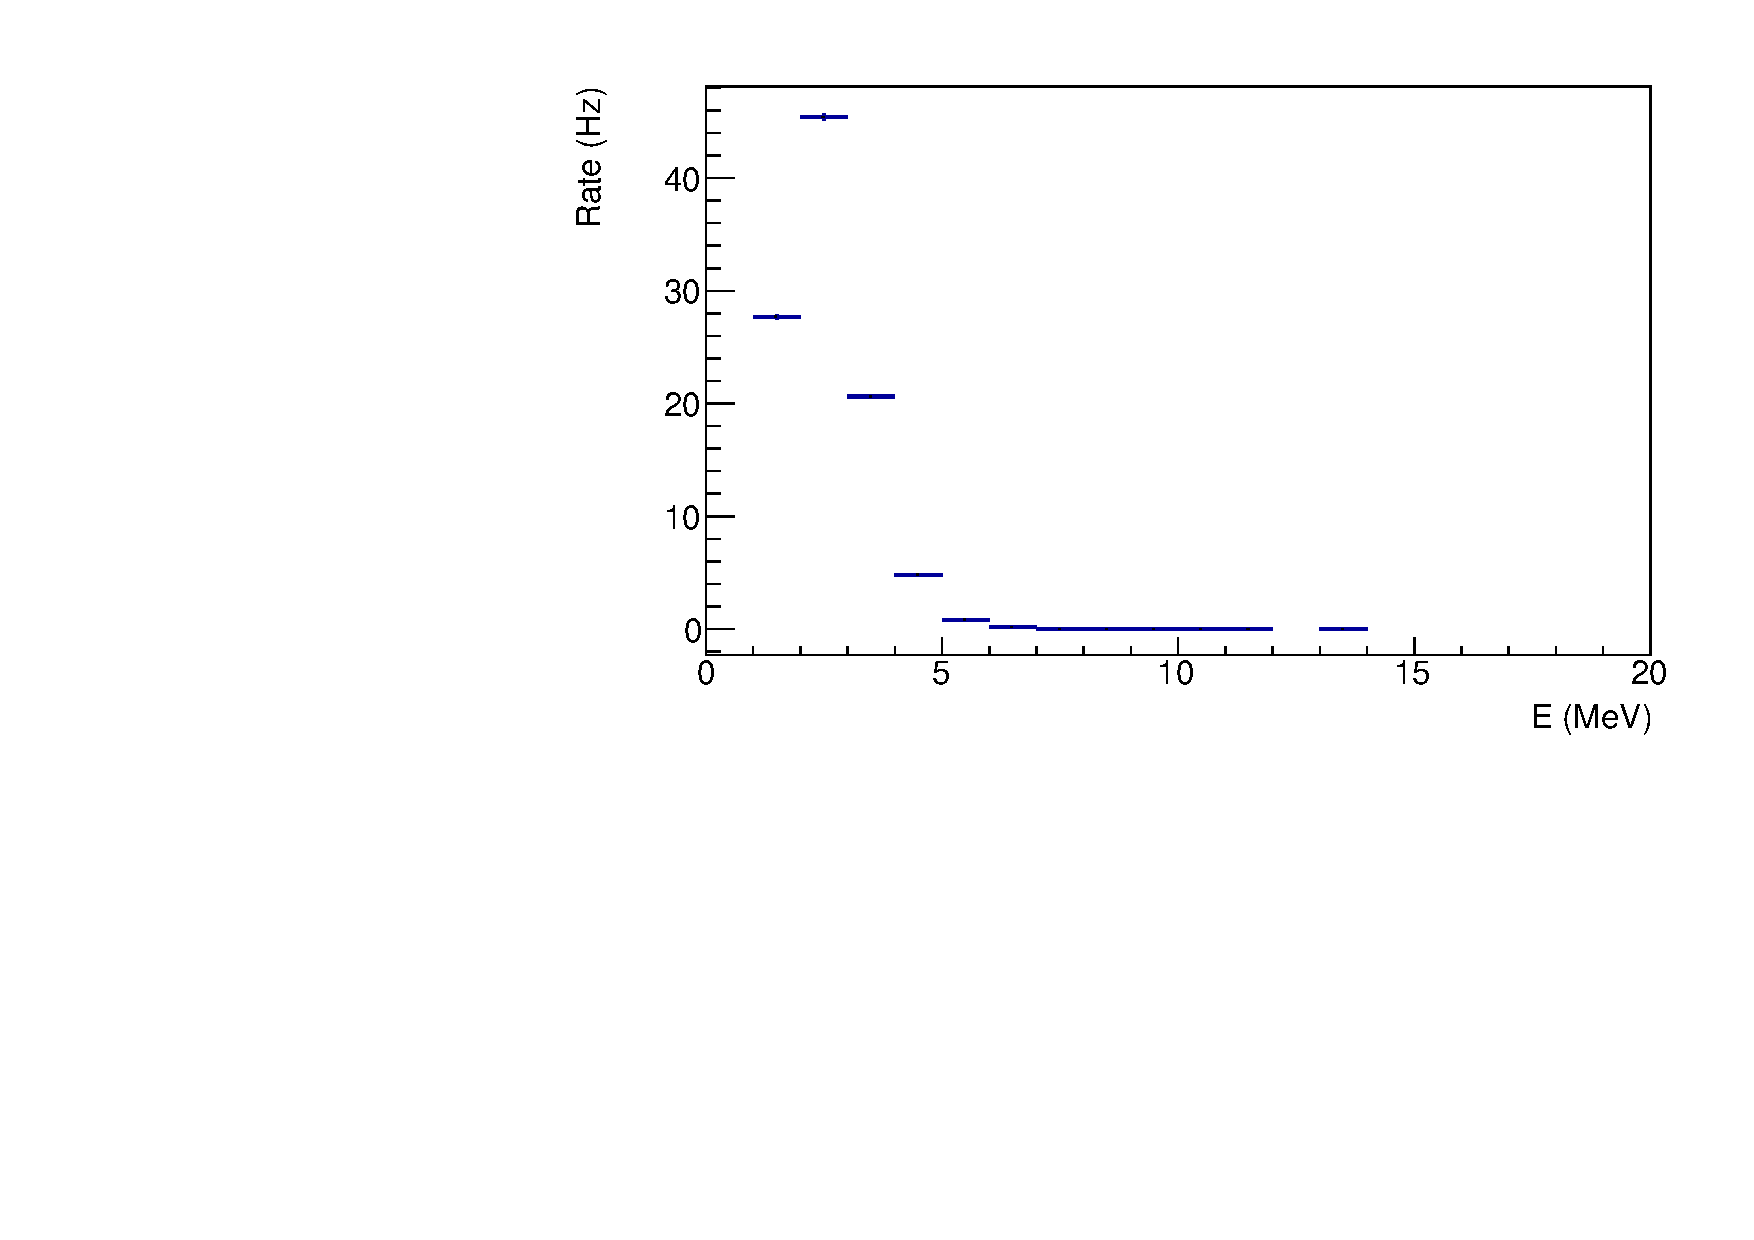
\includegraphics[width=65mm]{Figures/Cf252Multi.pdf}}
\caption[The segment hit multiplicity of calibration gamma clusters]{The segment hit multiplicity of gamma clusters from calibration sources: (a) $^{137}$Cs, (b) $^{22}$Na, (c) $^{60}$Co, (d) $n$-H capture gamma from $^{252}$Cf.
}
\label{fig:gammamulti}
\end{figure}

The $^{12}$B are mainly produced by cosmogenic neutrons with $^{12}$C(n, p)$^{12}$B interactions, whose cross-section is $\sim 0.01$ barn. 
Because the $\beta$ energy distribution covers a similar range as the IBD prompt energy, $^{12}$B is a valuable calibration source to characterize the reconstructed energy scale for an IBD prompt event's energy.
To select $^{12}$B events in PROSPECT, the time coincidence between a prompt neutron recoil signal and a delayed $\beta$ signal.
The prompt and delayed signal are also required to be adjacent.
A prompt signal is a single-segment hit with neutron-like PSD in the energy ranging from 0.7~MeV$_{ee}$ to 10~MeV$_{ee}$.
A delayed signal has gamma-like PSD with energy less than 15 MeV and multiplicity $< 3$ .
The $\Delta t$ between the prompt recoil and the delayed electron events is the range of (3, 30) ms to exclude neutron capture events. 
All delayed events are required to be $<12$~cm from the prompt events. 
The lifetime of $^{12}$B was measured as $28.8\pm0.6$ ms, agreed with the nominal $29.14$~ms lifetime recorded in the ENSDF database, as shown in Figure \ref{fig:B12plots}. 
The prompt to delay distance is fitted with a Gaussian function whose the best fit standard deviation $\sigma_d$ = 2.91~cm.
The value of prompt and delay proximity cut, $\Delta z < 12$~cm, is set to minimize time variation of event selection efficiency, because the position resolution of the detector evolves with time.
In 73~days reactor off data acquisition, there are $\sim 35300$ $^{12}$B beta counted in PROSPECT AD with S:B=0.87. 
The reconstructed spectrum of $^{12}$B electrons is shown in Figure~\ref{fig:B12plots}.
Because of the short traveling distance of MeV-scale betas, $^{12}$B events are dominated by beta particles with multiplicities equal to one.
\begin{figure}[h!]
\centering
\subfigure[]{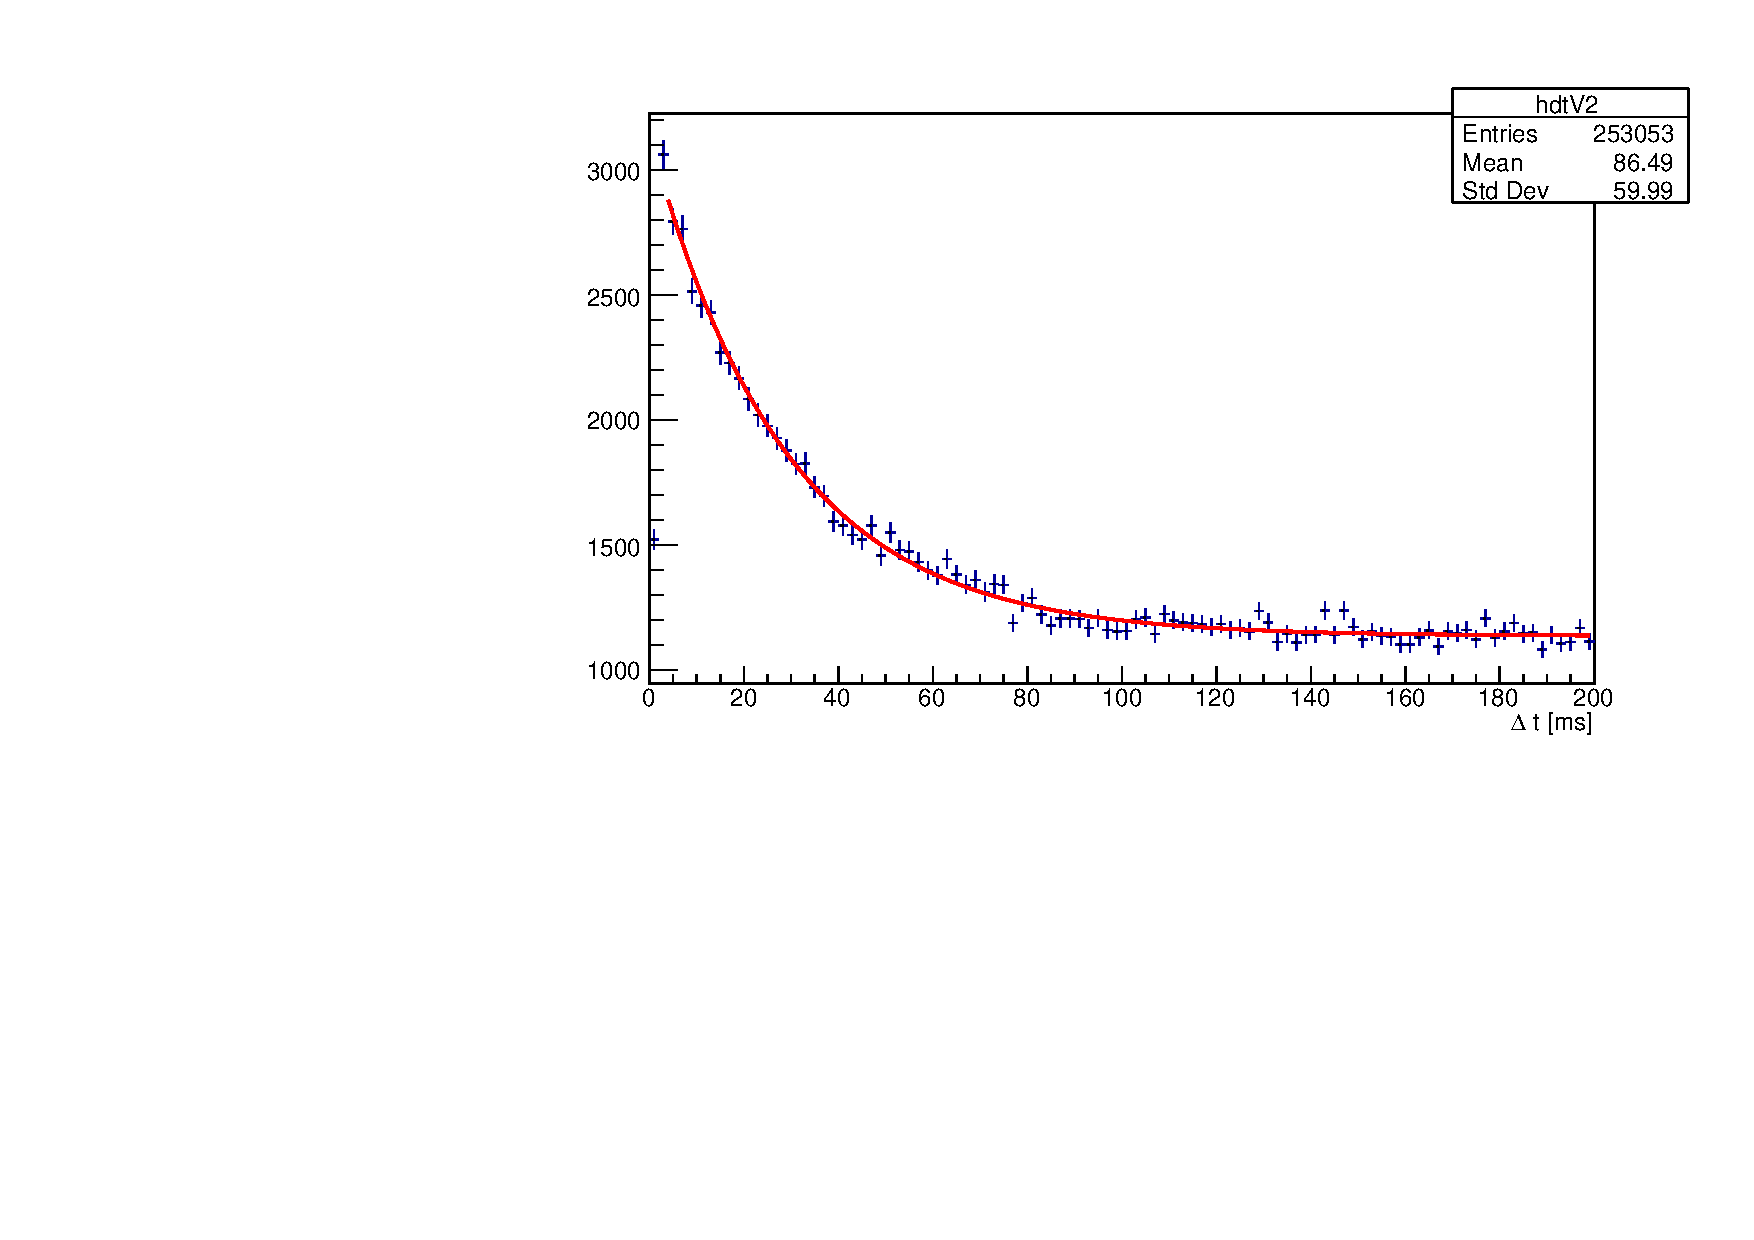
\includegraphics[width=60mm]{Figures/B12dt85.pdf}}\quad
\subfigure[]{\label{fig:distance}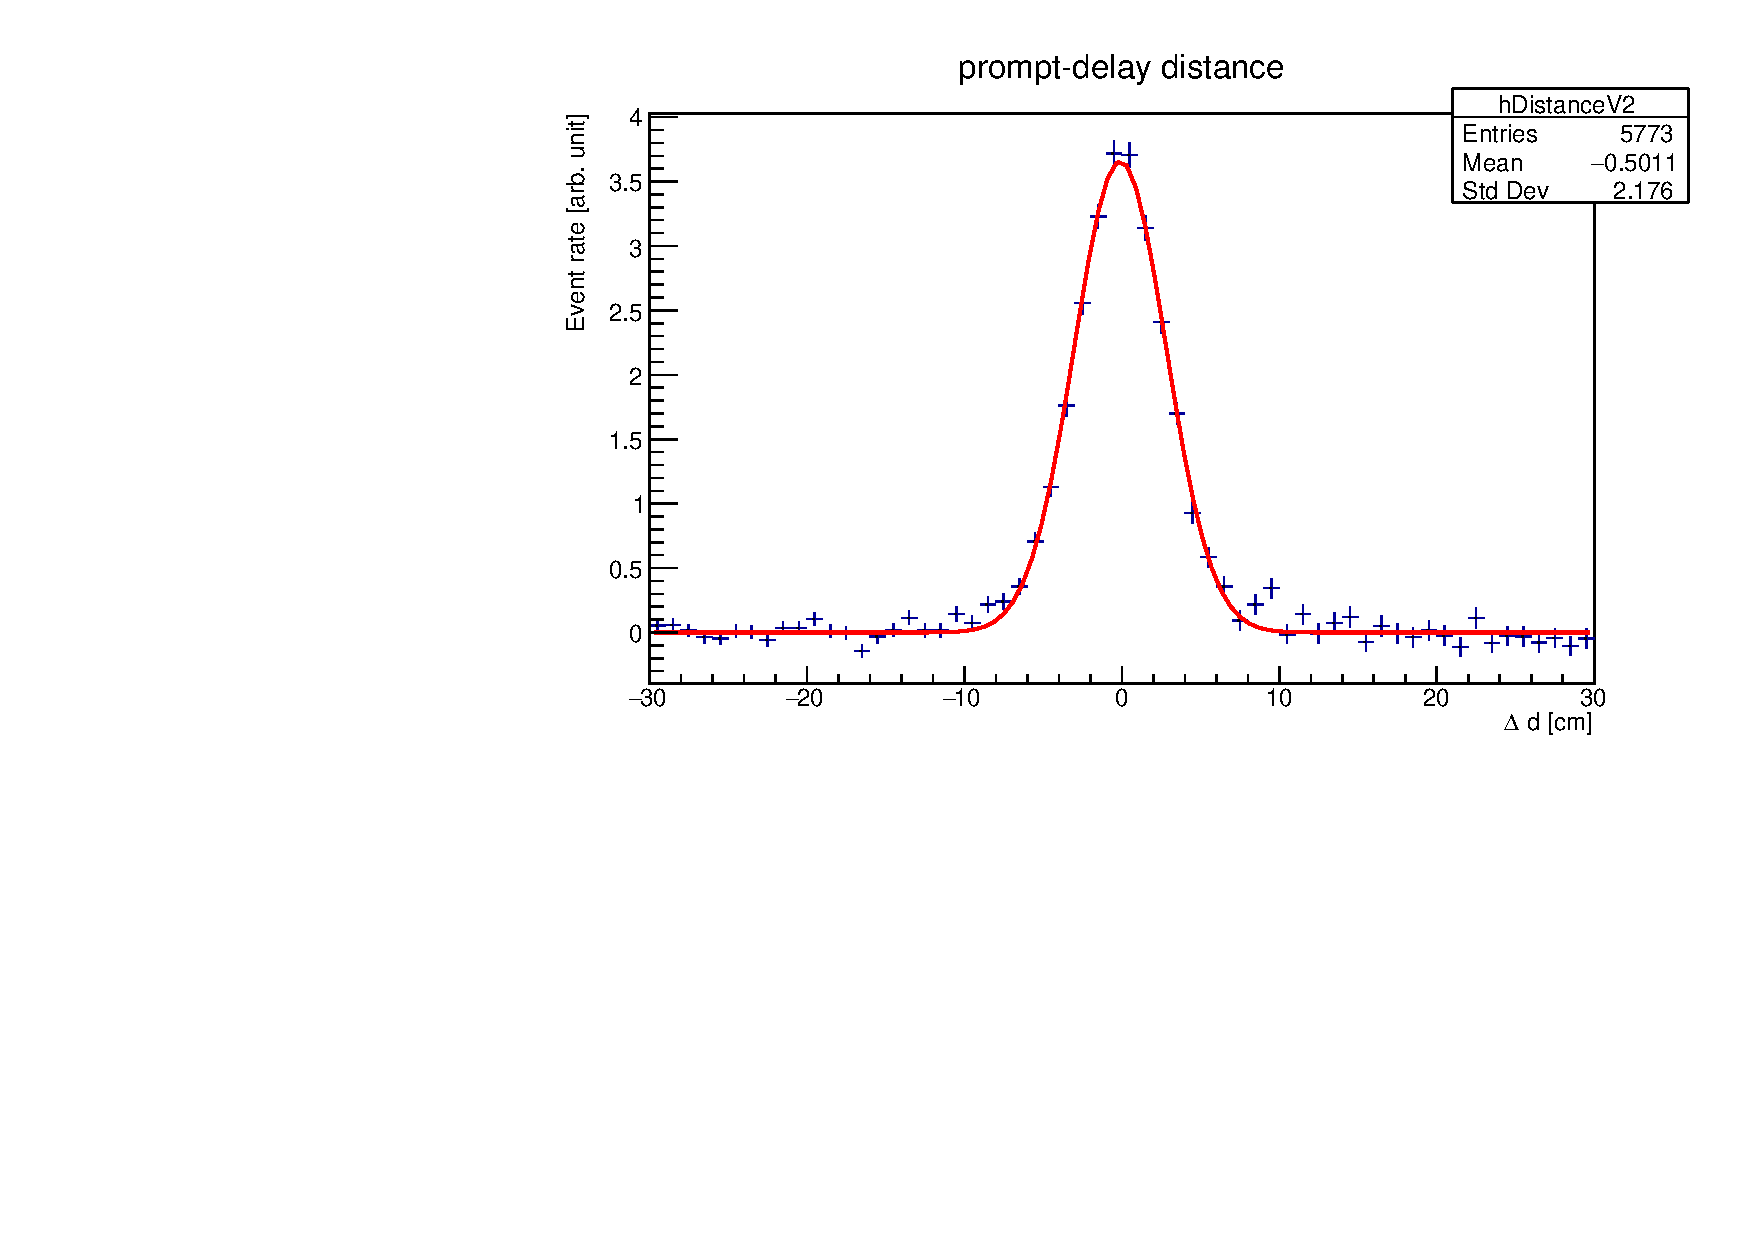
\includegraphics[width=60mm]{Figures/B12distance85.pdf}} \\
\subfigure[]{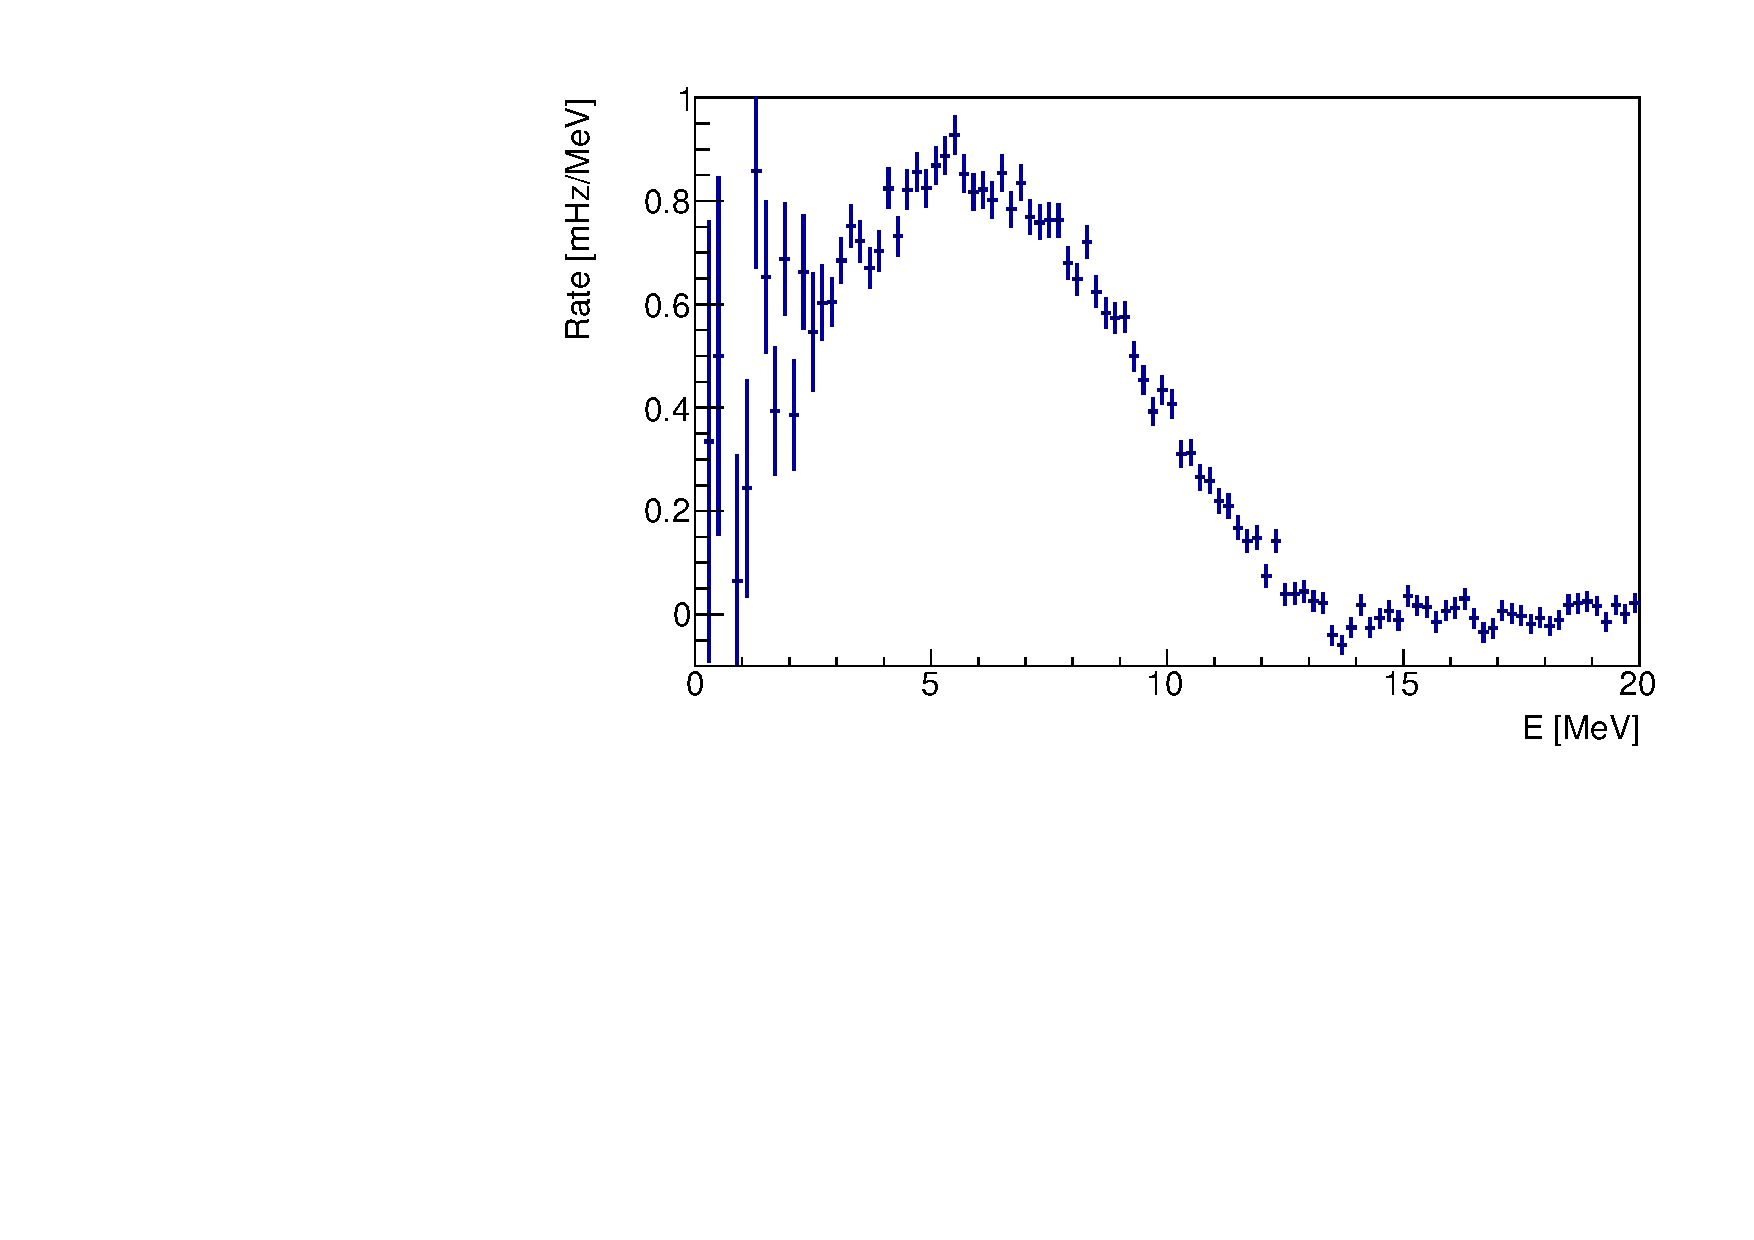
\includegraphics[width=60mm]{Figures/B12smear90.pdf}} 
\subfigure[]{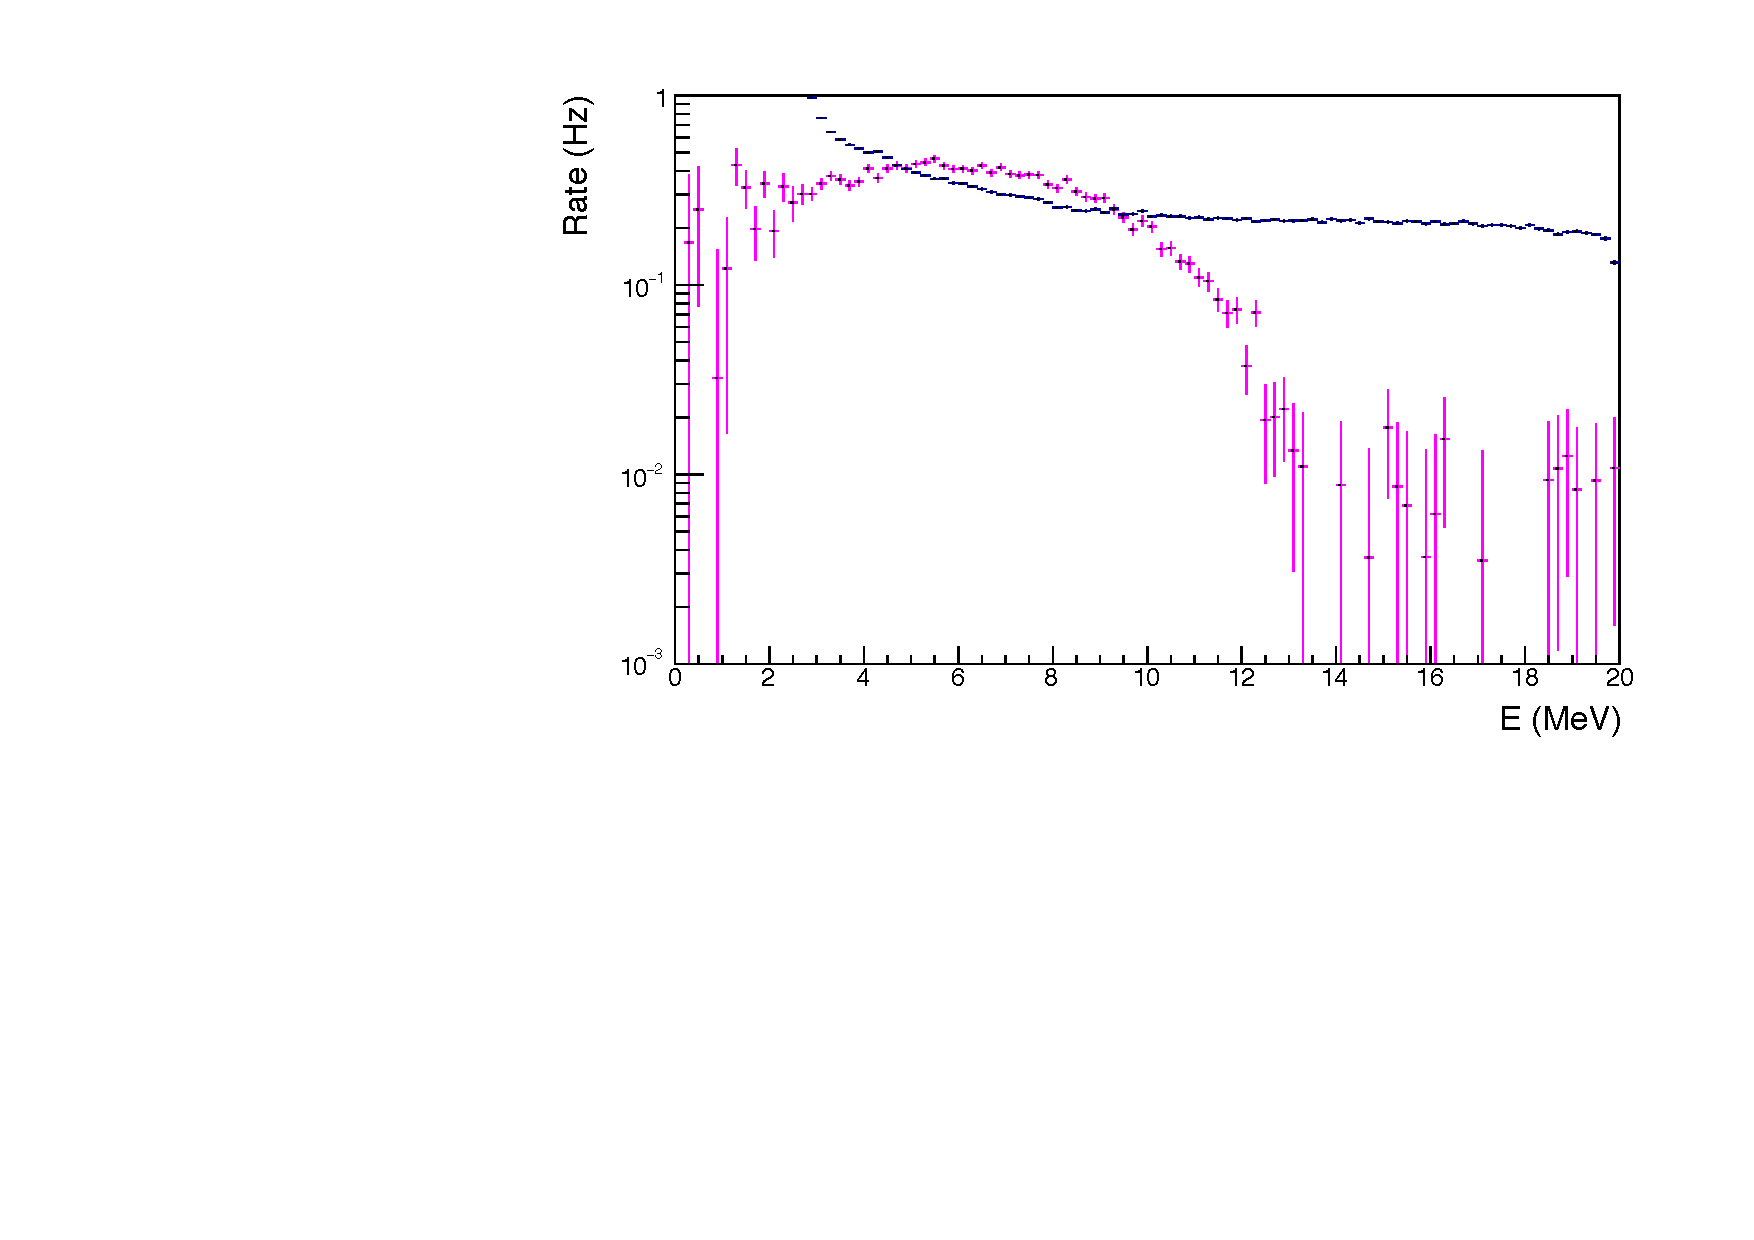
\includegraphics[width=60mm]{Figures/B12BG.pdf}} 
\caption[The observed of $^{12}$B spectrum in PROSPECT]{The observed of $^{12}$B spectrum in PROSPECT. (a) The delay-prompt time difference of $^{12}$B candidates  (b)The delay-prompt distance of $^{12}$B candidates. (c) The reconstructed $^{12}$B spectrum. (d) The $^{12}$B signal spectrum (pink) compared to the background spectrum (blue).}
\label{fig:B12plots}
\end{figure}

The AmBe calibration source is a composite neutron source, where the $\alpha$ emitted from $^{241}$Am interacts with $^9$Be through
\begin{equation}
	\alpha + ^9\textrm{Be} \rightarrow n + ^{12}\textrm{C} + 4.4 \textrm{MeV}
\end{equation} 
with a 4.4~MeV single energy gamma emission.
Although the AmBe calibration data was not included in the data of PROSPECT's neutrino spectrum measurement, the 4.4~MeV gamma is a good cross check for PROSPECT to show its capability to reconstruct particles in the 4~MeV to 6~MeV energy range, where the IBD prompt spectrum distortion was found.
The single energy gamma is selected based on the time coincidence between the gamma-like prompt signal and the delayed $n$-Li capture signal using the discrimination with PSD.
A challenge in the AmBe event selection is that the neutron produced from $\alpha$-Be collision has a 1~MeV scale kinetic energy, causing non-negligible signal mixing of the gamma and proton recoil in the prompt event cluster.
Therefore, the exclusion of proton recoil from the prompt cluster is necessary to purify reconstructed spectrum of the prompt 4.4~MeV gamma.
The energy spectrum of the AmBe gamma is shown in Figure~\ref{fig:AmBePlot}.

%\FloatBarrier
\begin{figure}[h!]
\centering
\subfigure[]{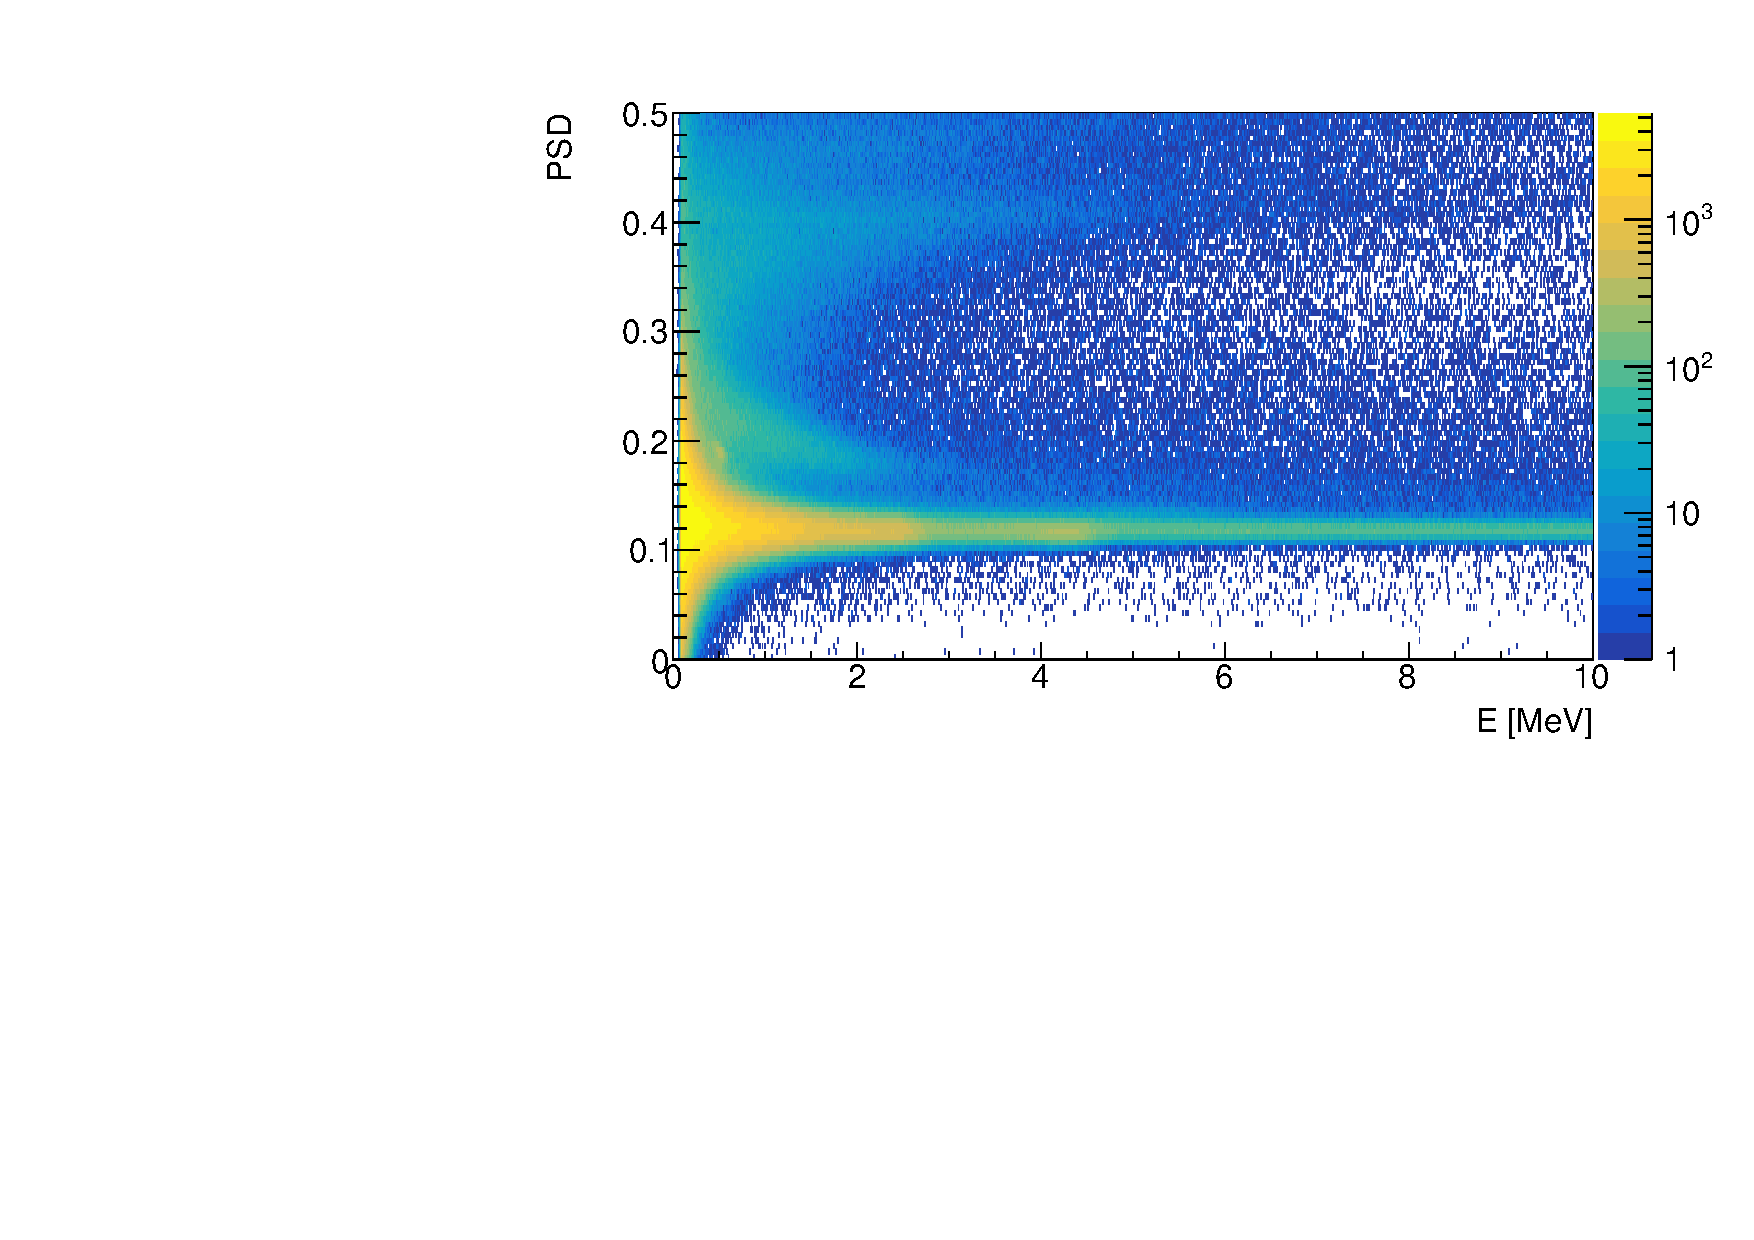
\includegraphics[width=0.45\textwidth]{Figures/AmBeDataPSD.pdf}}
\subfigure[]{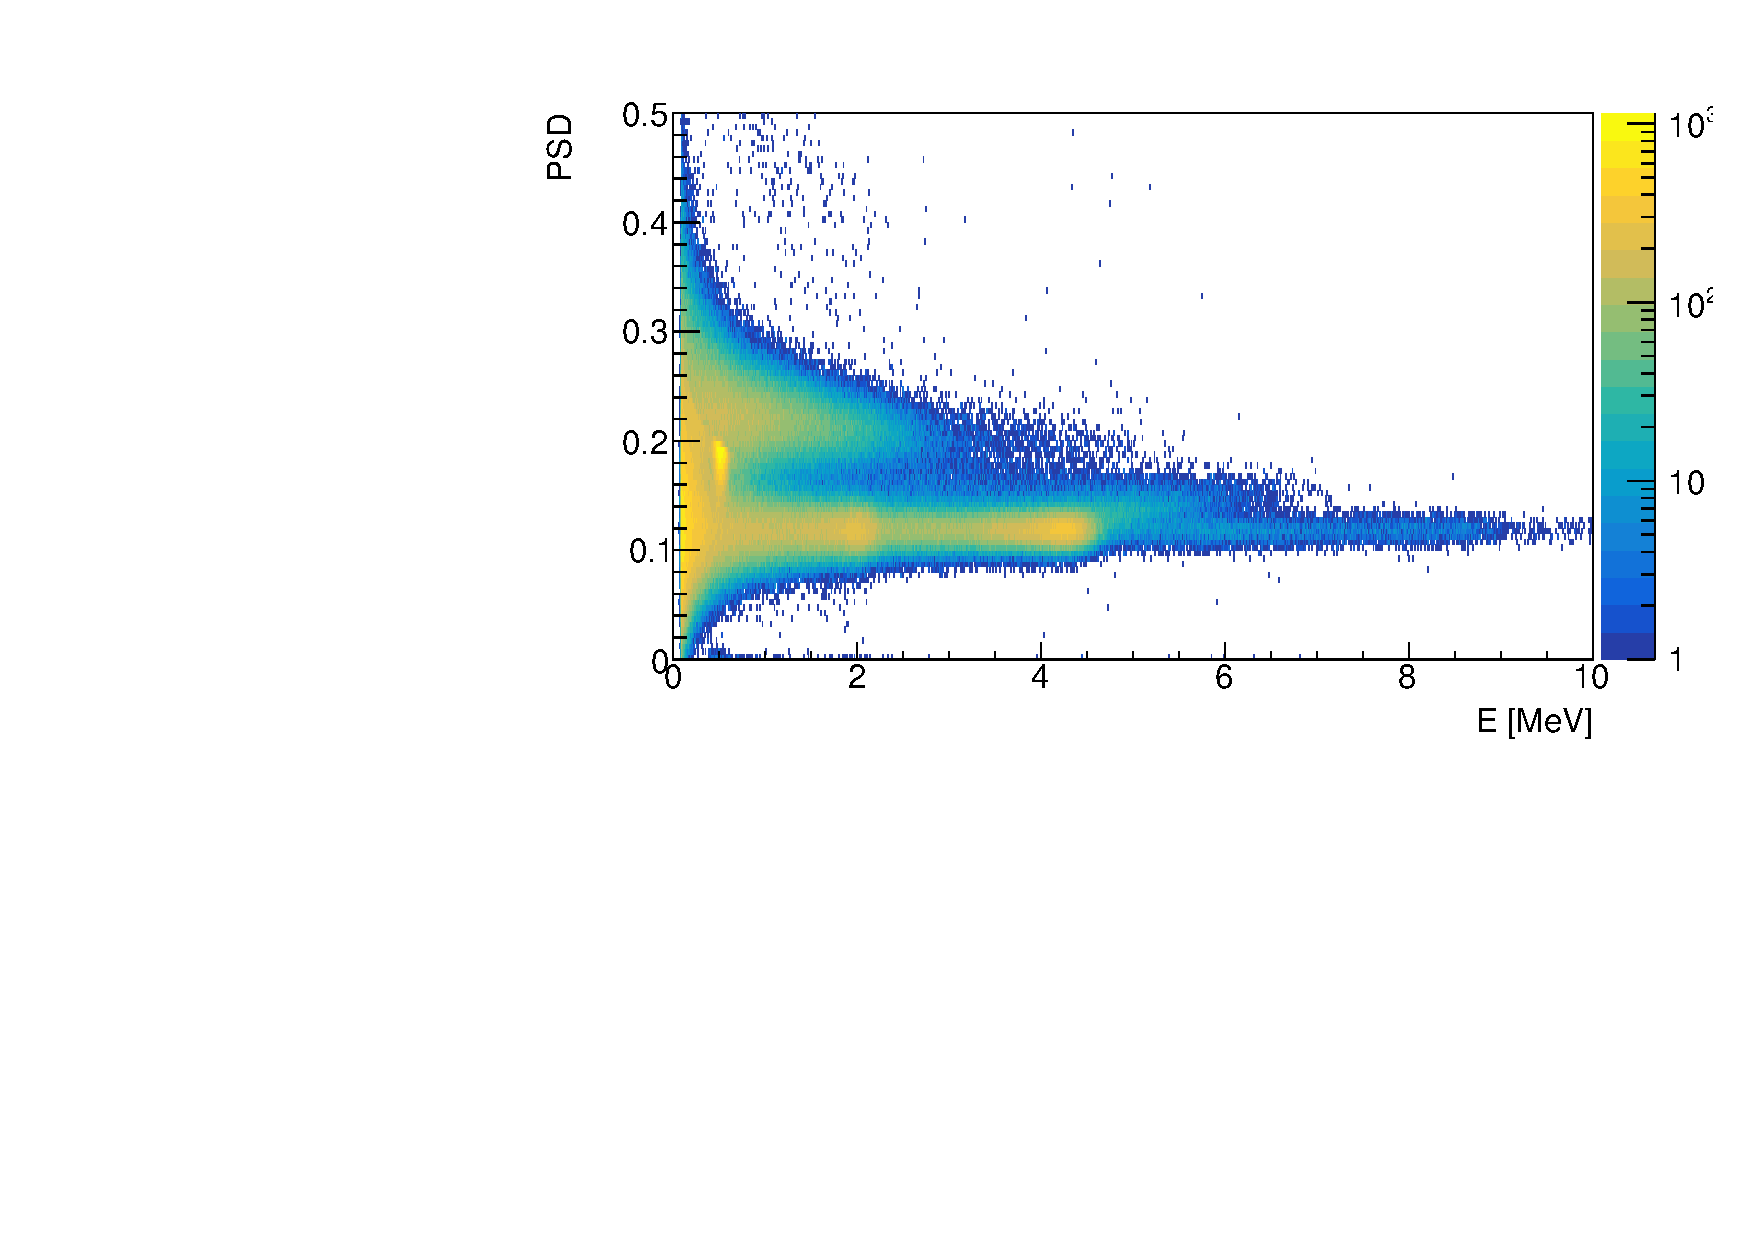
\includegraphics[width=0.45\textwidth]{Figures/AmBeMCPSD.pdf}}\\
\subfigure[]{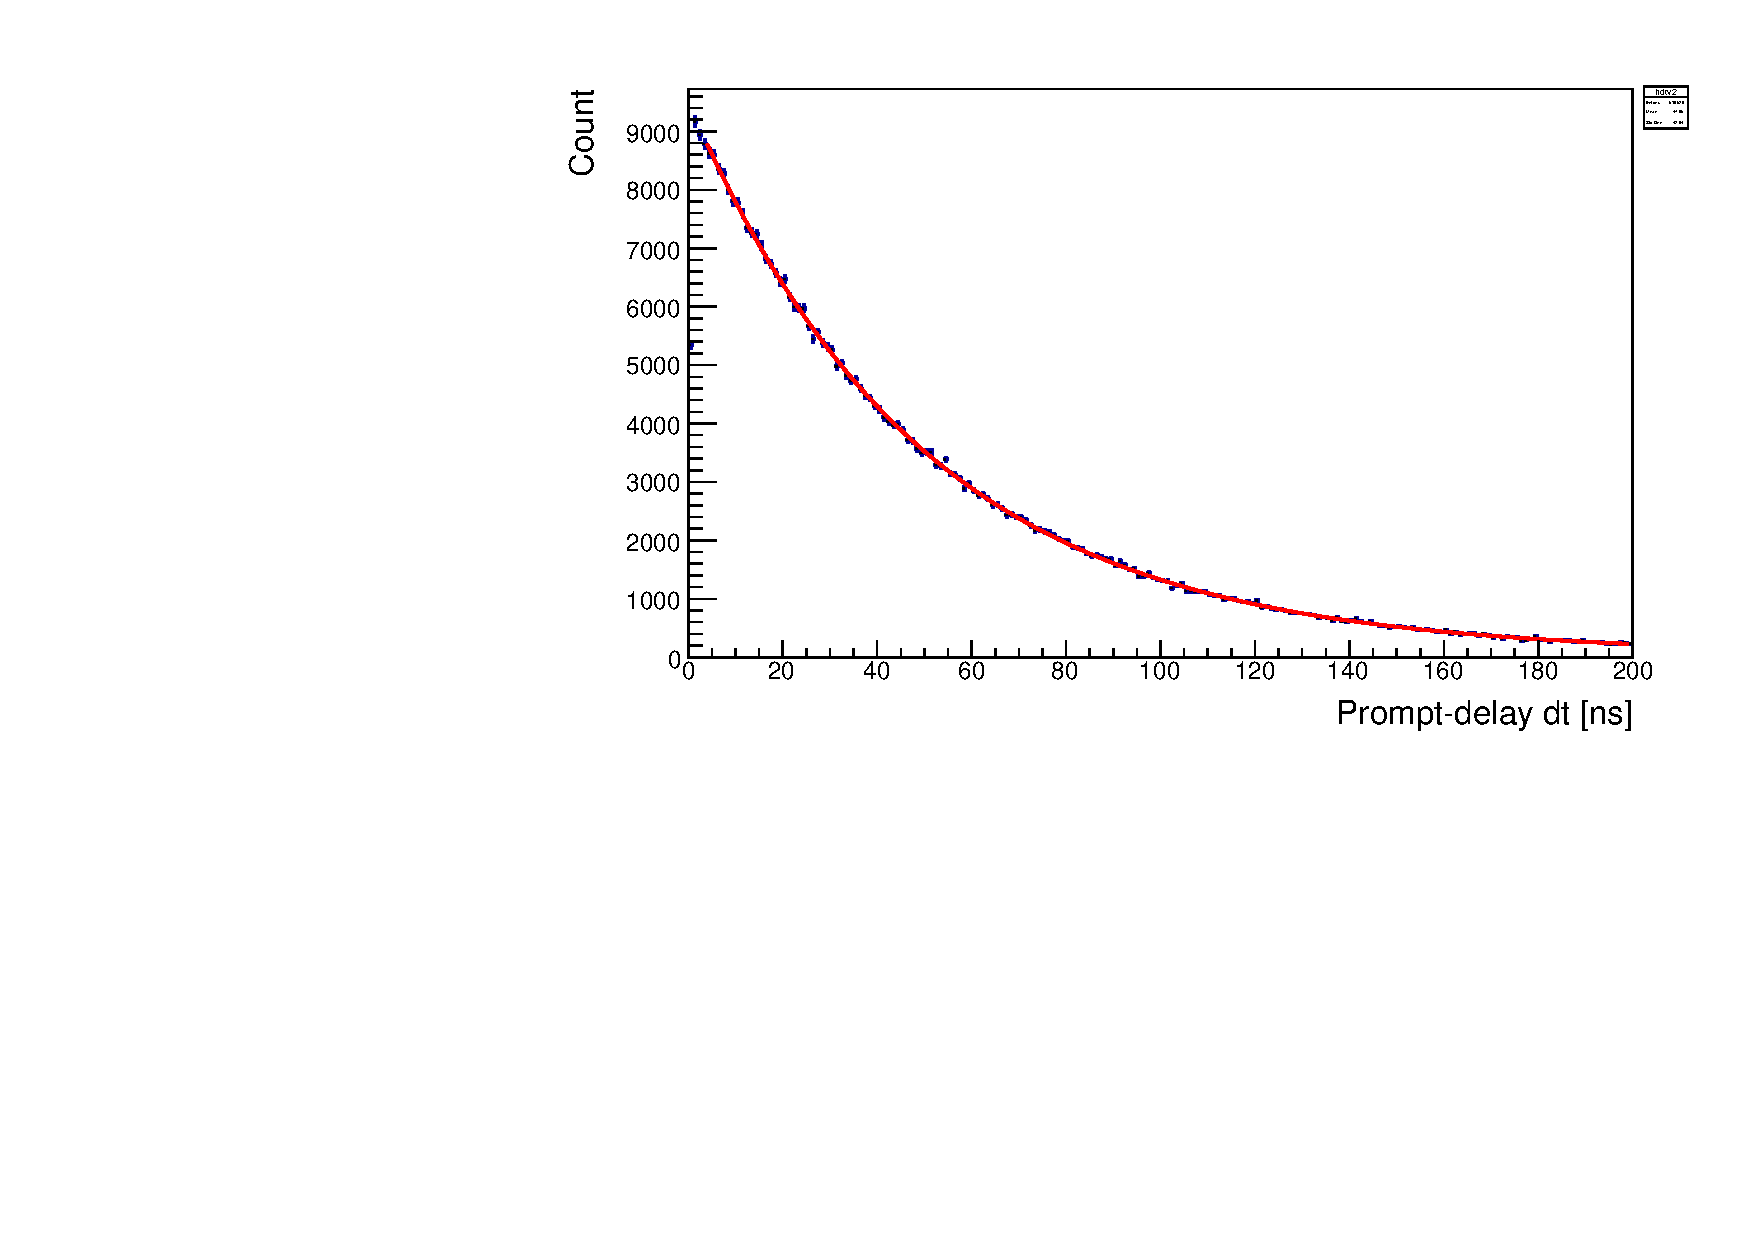
\includegraphics[width=0.45\textwidth]{Figures/AmBedt.pdf}}
\subfigure[]{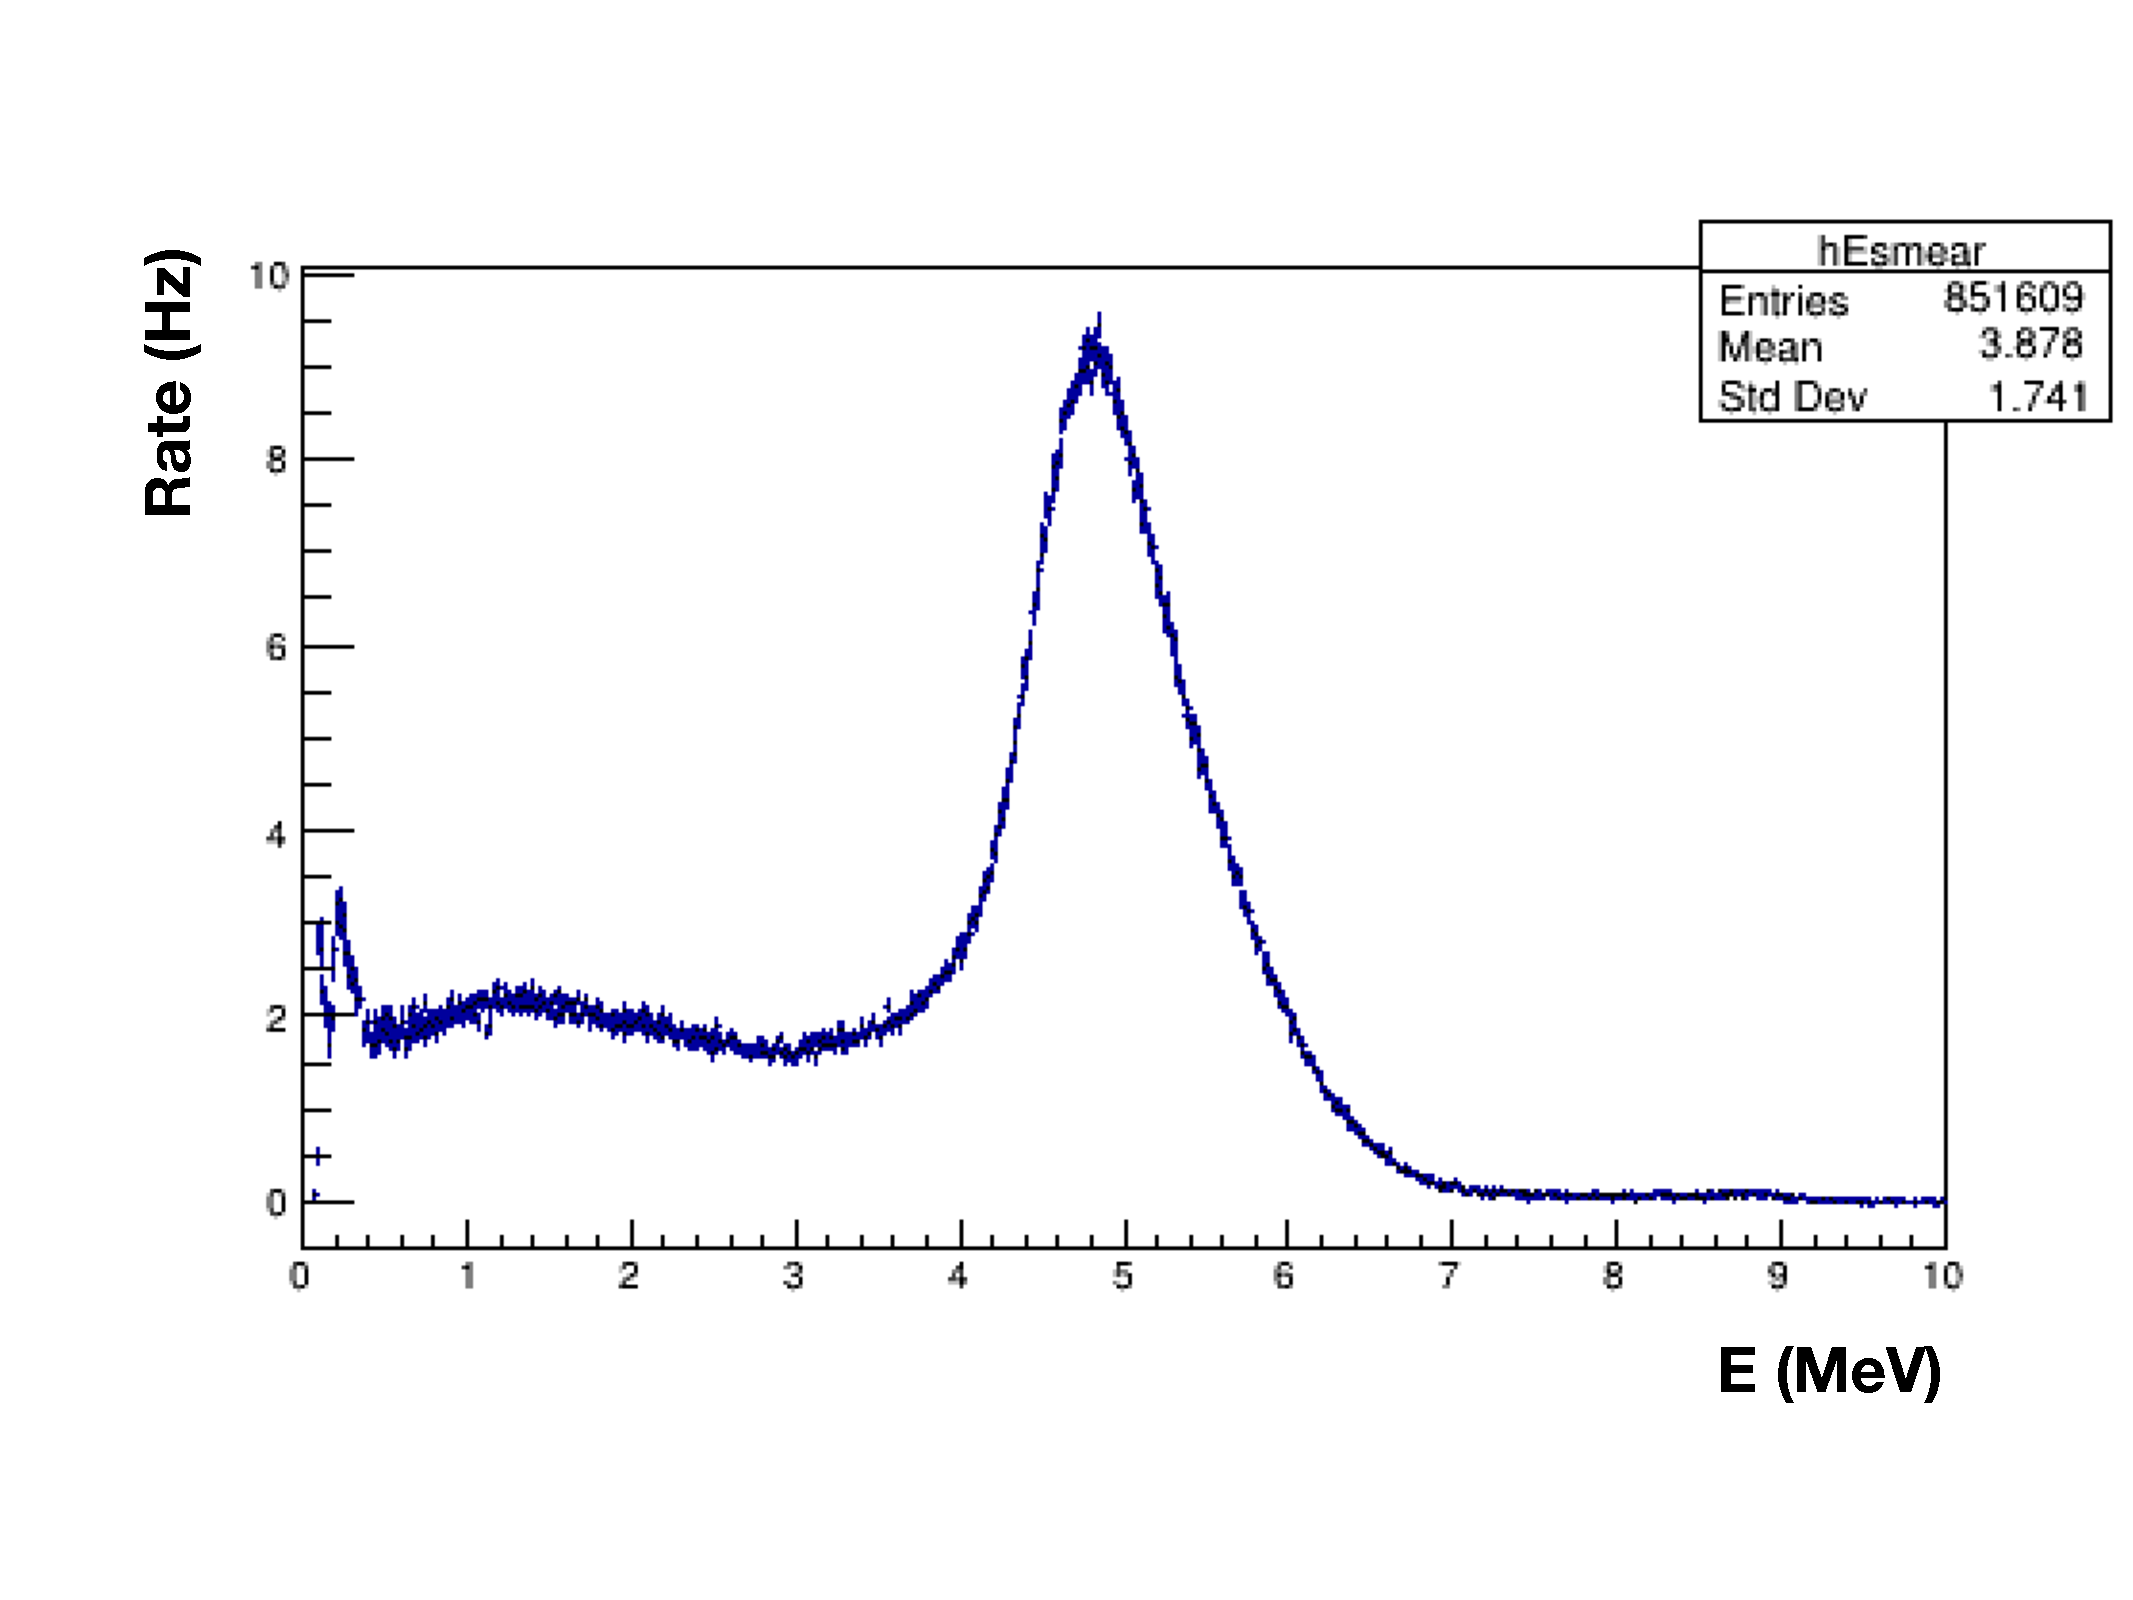
\includegraphics[width=0.45\textwidth]{Figures/AmBeWRecoil.pdf}}\\
\subfigure[]{\includegraphics[width=0.49\textwidth]{Figures/AmBesmear90.pdf}}
\caption[AmBe gamma reconstruction]{(a) and (b) The PSD distribution of all hits detected in the AmBe calibration and simulation, where the gamma PSD distribution is distorted because of the mixing of gamma and prompt proton recoil from the Be($\alpha$, n)C interaction.
	(c) The best fit neutron life time of be AmBe data equals to 49.7~ns.
	(d) The reconstructed energy of the AmBe prompt events without the exclusion of prompt recoil-like hits.
	(e) The reconstructed energy of the AmBe gamma after strict exclusion of prompt recoil-like hits.}
\label{fig:AmBePlot}
\end{figure}
%\FloatBarrier

\Section{Monte-Carlo Simulation of Calibrations}

The purpose of comparing calibration data to MC simulation is to characterize the detector energy response and  produce PROSPECT's expected IBD spectrum.
The difference between the deposited energy and the reconstructed energy is the result of multiple physical effects in the PROSPECT AD.
The Birks' quenching effect and the Cherenkov radiation can cause nonlinear energy reconstruction.
Dead volume in the detector contributed by the optical grid also affects the reconstructed energy with gamma leakage and energy loss.
In addition, there are relative energy scale differences among segments that are caused by non-uniformity of LS and segment volume.
The resolution of reconstructed energy is dominated by  the photostatistics of LS.
To eliminate the time dependence of the energy resolution, both data and MC events' energies are smeared with respect to the poorest energy resolution (lowest PE/MeV) found during the production data and throughout the detector.

In PG4 simulation, the Birk’s constant, $k_{B1}$ and $k_{B2}$, the detection efficiency of Cherenkov light $k_{C}$, and a absolute energy scale $A$ are the terms used to quantify the energy nonlinearity model and the energy scale.
The MC reconstructed energy is  
\begin{equation}
E_{MC} = \sum_i^{steps} A(E_{quench,i}(k_{B1},k_{B2})+E_{Ckov,i}(k_c)),
\end{equation}
where $E_{quench,i}(k_{B1}, k_{B2})$ is the effective quenched energy whose magnitude is determined by the Birks' constants, and $E_{Ckov,i}(k_c)$ is the effective Cherenkov radiation's contribution to the reconstructed energy.

The nonlinearity caused by the ZLE threshold, detector geometry, and other effects are also described in this section.

\Subsection{Nonlinearity Factors}
\label{sec:nonlinear}

The nonlinear energy response of $^6$LiLS is mainly the result of the Birks$^\prime$ quenching and Cherenkov radiation. 
The Birks' quenching constants $k_{B1}$ and $k_{B2}$ are user defined parameters to model the unique quenching effect for PROSPECT.
In Eq.~\ref{eq:birkslaw} and \ref{eq:birksMC} in Chapter~\ref{Ch6}, PG4 simulates the quenching effect by multiplying the energy difference in between \texttt{G4Step}s with a Birks' factor:
\begin{equation}
   E_{quench} = \sum_{i}^{steps}\frac{\frac{dE_i}{dx}}{1+k_{B1}\frac{dE_i}{dx}+k_{B2}(\frac{dE_i}{dx})^2}.
   \label{eq:birks}
\end{equation}
The nonzero value of $k_{B1}$ reduces the reconstructed energy of lower energy events, as illustrated in Figure~\ref{fig:kb1plot}.
Although $k_{B2}$'s effect is negligible in higher energy, it is capable of affecting particle segment-hit multiplicity through its ability to quench more lower energy events below the 90~keV threshold, as shown in Figure \ref{fig:kb2plot}.

\begin{figure}[h!]
\centering
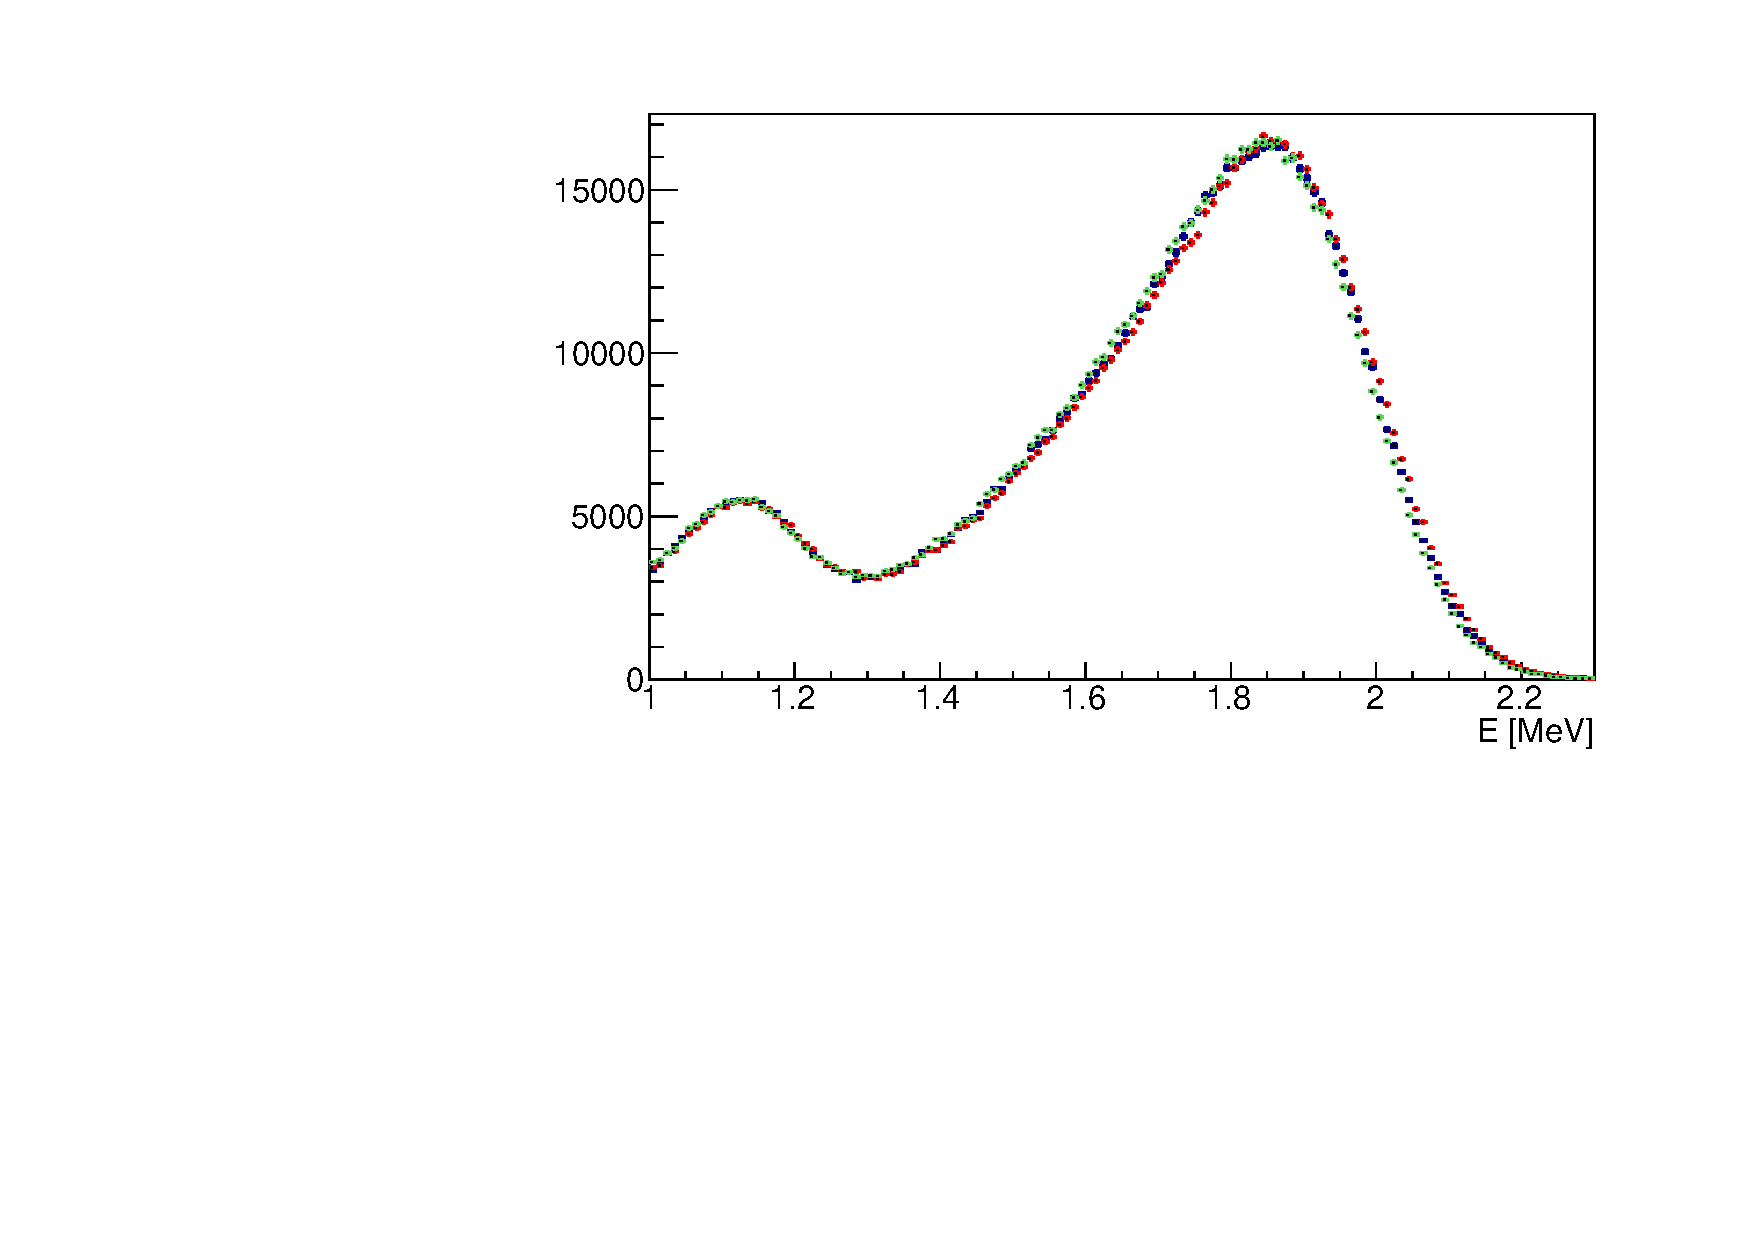
\includegraphics[width=0.7\textwidth]{Figures/kb1.pdf}
\caption[Quenched energy affected by different $k_{B1}$ values]{The MC quenched energy affected by different $k_{B1}$ values. (red:  $k_{B2} = 0.124$~mm/MeV, blue: $k_{B2} = 0.132$~mm/MeV, green: $k_{B2} = 0.140$~mm/MeV)}
\label{fig:kb1plot}
\end{figure}
 
\begin{figure}[h!]
\centering
\subfigure[]{\label{fig:kb2}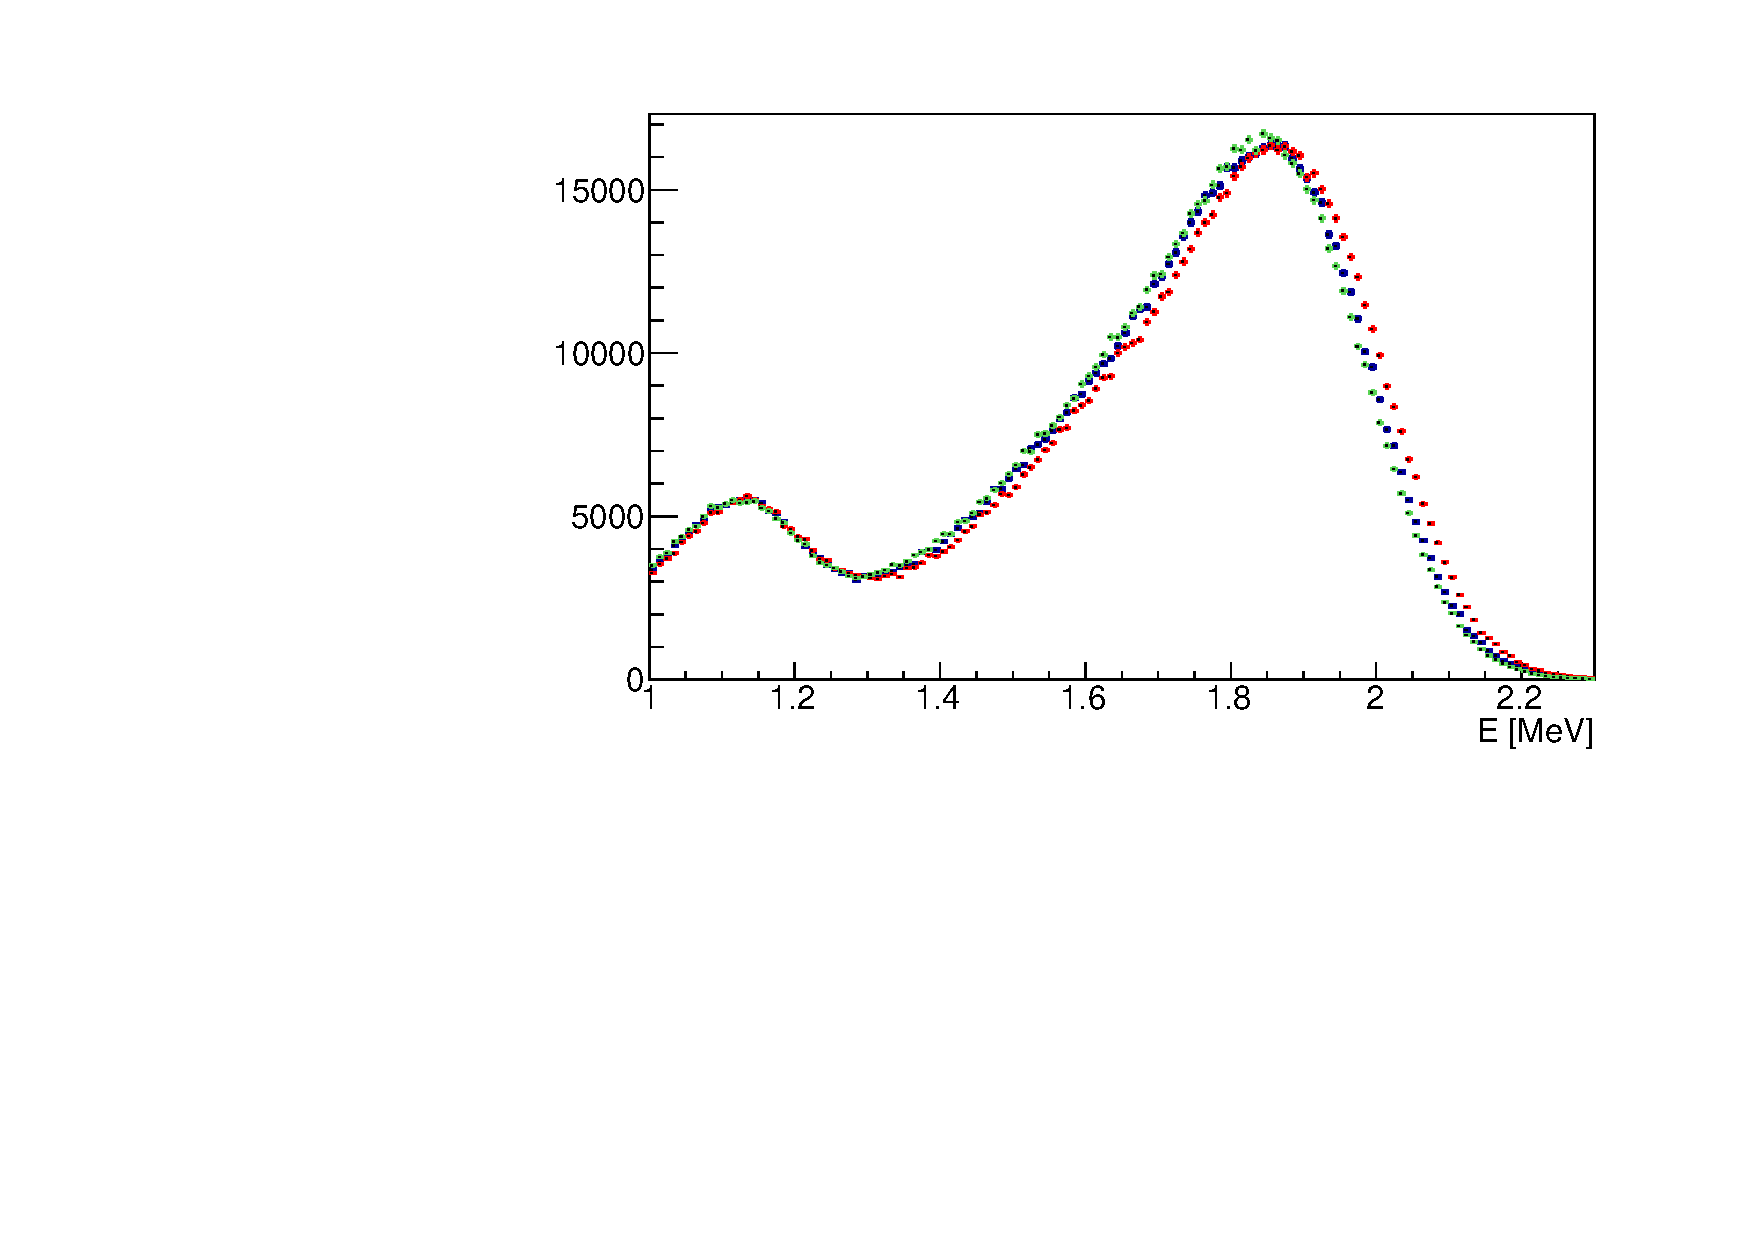
\includegraphics[width=0.45\textwidth]{Figures/kb2.pdf}}\quad
\subfigure[]{\label{fig:kb2multi}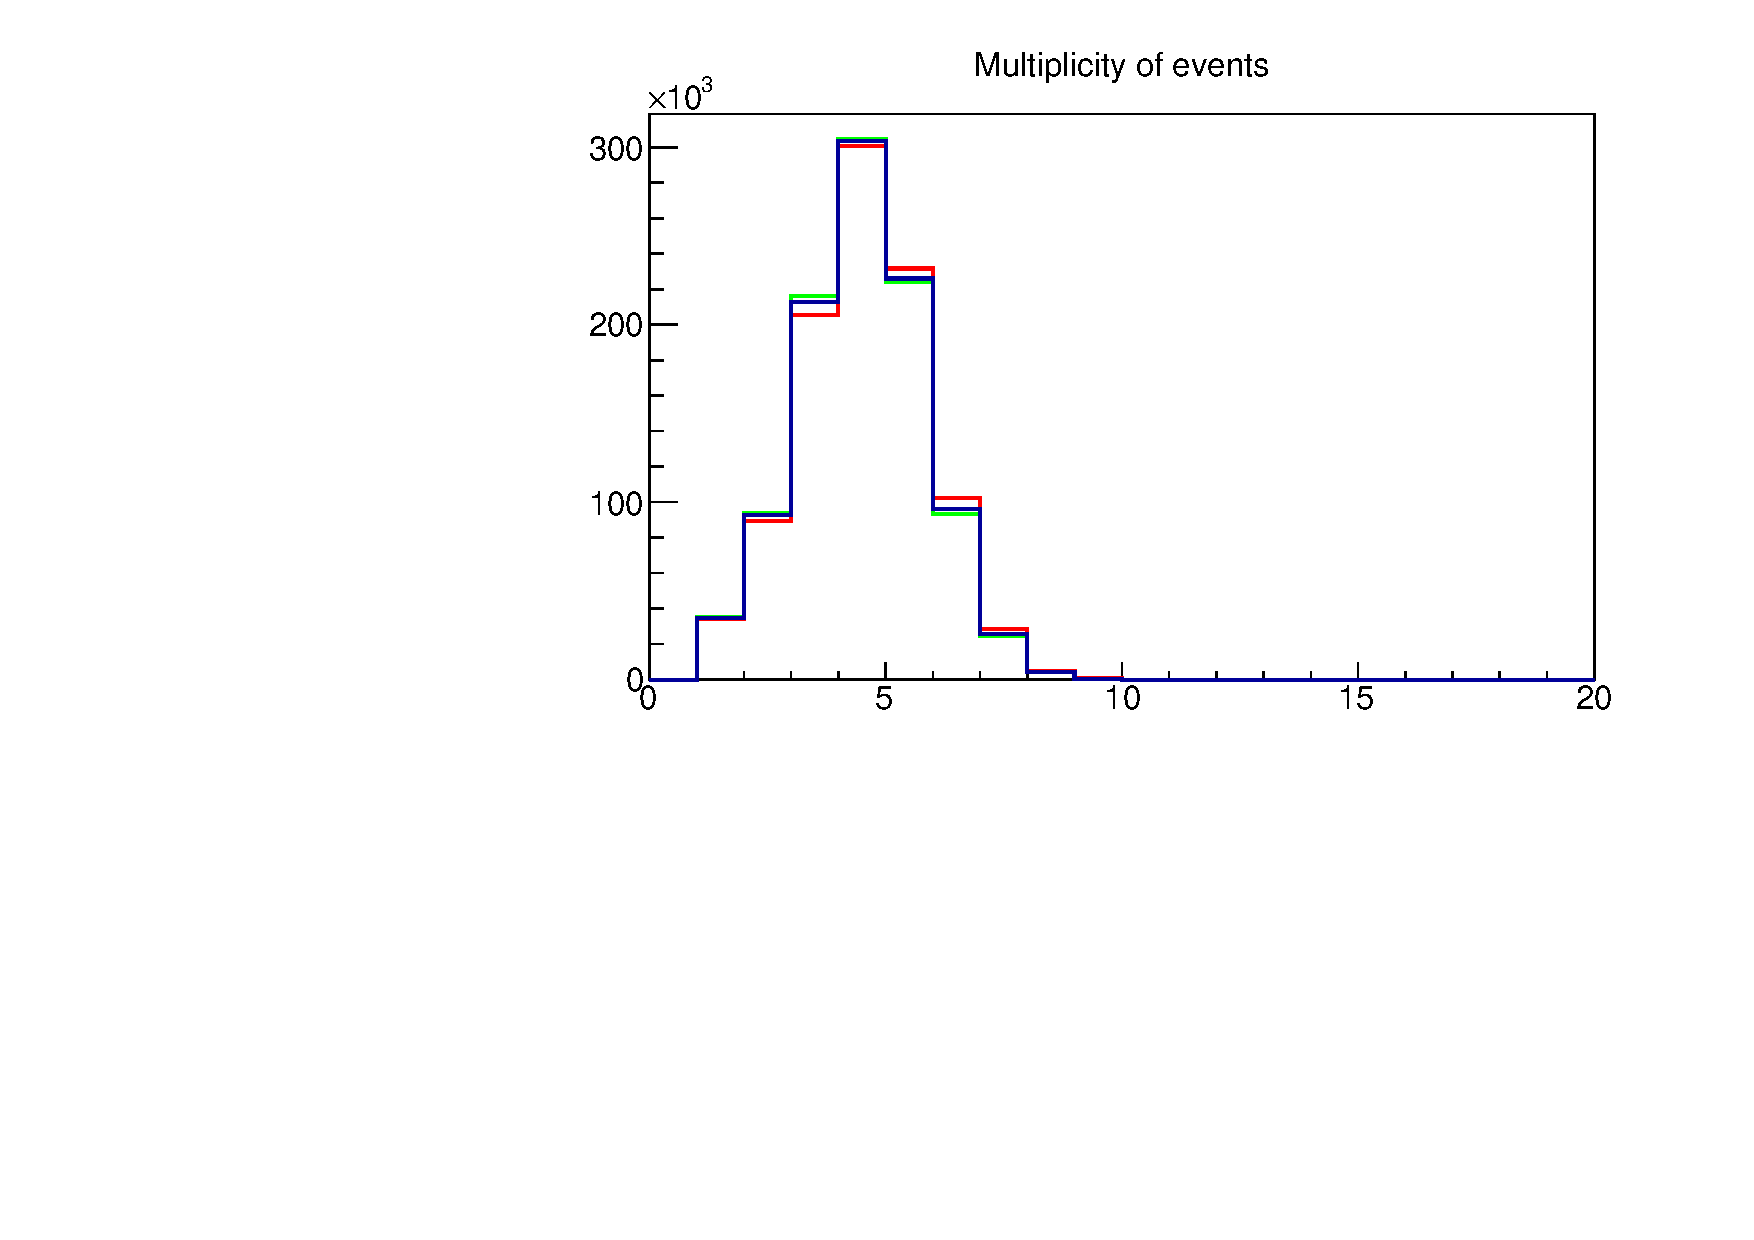
\includegraphics[width=0.45\textwidth]{Figures/kb2multi.pdf}}
\caption[Quenched energy affected by different $k_{B2}$ values]{The MC quenching induced by $k_{B2}$. (a) The energy distribution of $^{22}$Na simulation affected by $k_{B2}$. (b) The $^{22}$Na cell-hit multiplicity affected by $k_{B2}$.  (red: $k_{B2} = 0.015$~mm/MeV, blue: $k_{B2} = 0.023$~mm/MeV, green: $k_{B2} = 0.031$~mm/MeV)}
\label{fig:kb2plot}
\end{figure}

According to Chapter~\ref{Ch6}, the number of photon generated along the particle track is expressed as
\begin{equation}
    \frac{d^2N}{dxd\lambda} = \frac{2\pi\alpha z^2}{\lambda}\left(1- \frac{1}{\beta^2n^2(\lambda)}\right),
    \label{eq:ckov}
\end{equation}
where $N$ is number of photons, $\alpha$ is the fine structure constant, $z$ is the particle's electric charge, $\beta$ is the speed of the particle and $n(\lambda)$ is index of refraction.
Although most Cherenkov light is in the Ultraviolet (UV) wavelength range, the LS is able to absorb and re-emit it to VIS range with currently unknown efficiency.
Therefore, Cherenkov photons can be collected in addition to the scintillation light from high energy incident charged particles and increase reconstructed energy.
To simplify the MC simulation, the additional light emitted from the Cherenkov radiation is added to the reconstructed energy as the summed energy of detected Cherenkov photons,
\begin{equation}\label{eq:ceren2}
E_{ckov} = k_{c}\sum_{\lambda}N_\lambda E_\lambda,
\end{equation}
where $N_\lambda$ is number of photons per wavelength calculated by summing the number of Cherenkov photons in all \texttt{G4Step}s.
The LS's index of refraction and transmission spectrum are assumed to be constant for wavelengths in 200-700 nm range.
The effective light collection efficiency of Cherenkov photons, $k_{C}$, can be adjusted to model the effect of Cherenkov radiation on reconstructed energy. 
The particle energy loss due to Cherenkov radiation is negligible.
Figure \ref{fig:kcplot} shows different $k_{C}$ values affecting the n-H capture spectrum.

\begin{figure}[h!]
\centering
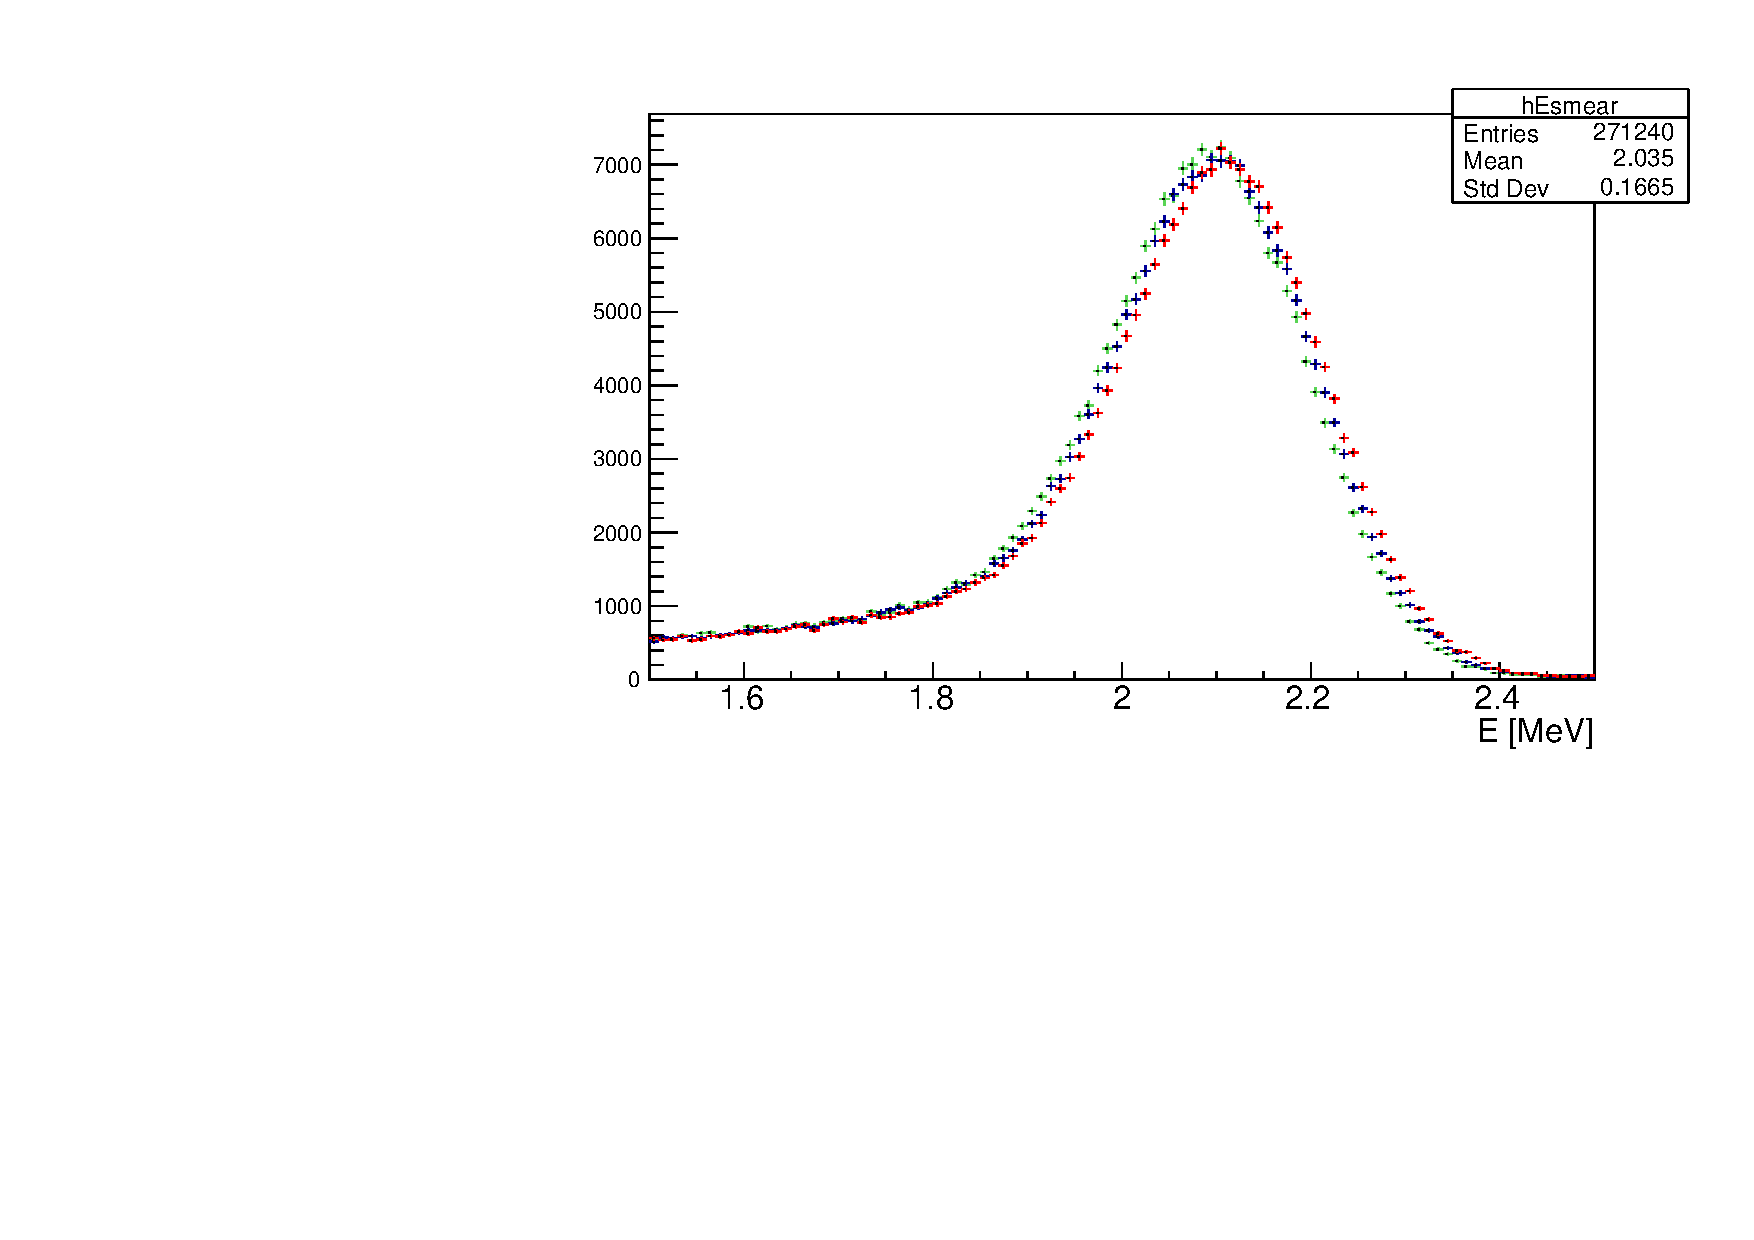
\includegraphics[width=0.7\textwidth]{Figures/kc.pdf}
\caption[The effect of Cherenkov radiation in PG4]{The MC Cherenkov radiation effect induced by $k_{C}$. (green:  $k_{C} = 30\%$, blue: $k_{C}= 35\%$, red: $k_{C} = 40\%$)}
\label{fig:kcplot}
\end{figure}

\Subsection{Energy Resolution}
\label{sec:resolution}
The reconstructed energy resolution is a function of energy:
\begin{equation}
\label{eql:resolution}
    \frac{\sigma}{E} = \sqrt{a^2 + \frac{b^2}{E}+\frac{c^2}{E^2}},
\end{equation}
where $a$ is affected by the detector geometry, $b$ is based on the photostatistics (PE/MeV) and $c$ represents the quantum efficiency of PMTs.
This energy dependent resolution function is widely used in evaluating the LS detectors' energy resolutions.
However, the PROSPECT AD's energy resolution is mainly affected by the energy resolution smearing of all hits and the low energy hit exclusion from multi-hit clusters caused by the ZLE threshold. 
The energy resolution characterized with the gamma calibration sources was not applied to the energy spectrum analysis.

\Subsection{Other Energy Scale  Factors}
\label{sec:other}
The reconstructed energy scale was initially based on the presumption that the reconstructed $n$-Li capture energy is 0.55 MeVee in detector. 
The deviation of the true electron equivalent energy to this estimation can induce a constant energy scale bias throughout the all energy. 
This absolute energy scale $A$, as a fitting parameter, was searched for best fit value simultaneously with other nonlinearity factors. 
The MINUIT $\chi^2$ minimization method~\cite{bib:minuit} is used to freely change $A$ until the $\chi^2$ between data and MC is minimized.

To ensure precise delta vs. MC comparisons, the ZLE threshold was simulated in the P2x data analysis package by converting the MC energy deposit in MC to pulse with respect to the ADC/PE ratio, as described in Chapter~\ref{Ch6}.
The 90~keV analysis ZLE threshold is then applied to the calibration MC using same P2x analysis program.

\Subsection{Detector Geometry Simulation}
The difference between the simulated detector geometry and the PROSPECT AD could lead to a disagreement in energy loss and gamma leakage between MC and data. 
The reconstructed energy of a multi-hit cluster is affected by the separator thickness, the PLA rods' size, and all dead volume contributing materials in the detector.
In this work, PG4's detector structure was simulated with detailed adjustments based on the actual design and measurements of the PROSPECT AD, including the thickness and chemical composition of separators, the PLA rods' dimensions, the structure of calibration system, the density and mixture of the LS and calibration capsule properties. 
PG4 simulated energy spectra with and without detailed detector structural match are shown in Figure~\ref{fig:PG4geometry}

\begin{figure}[h!]
\centering
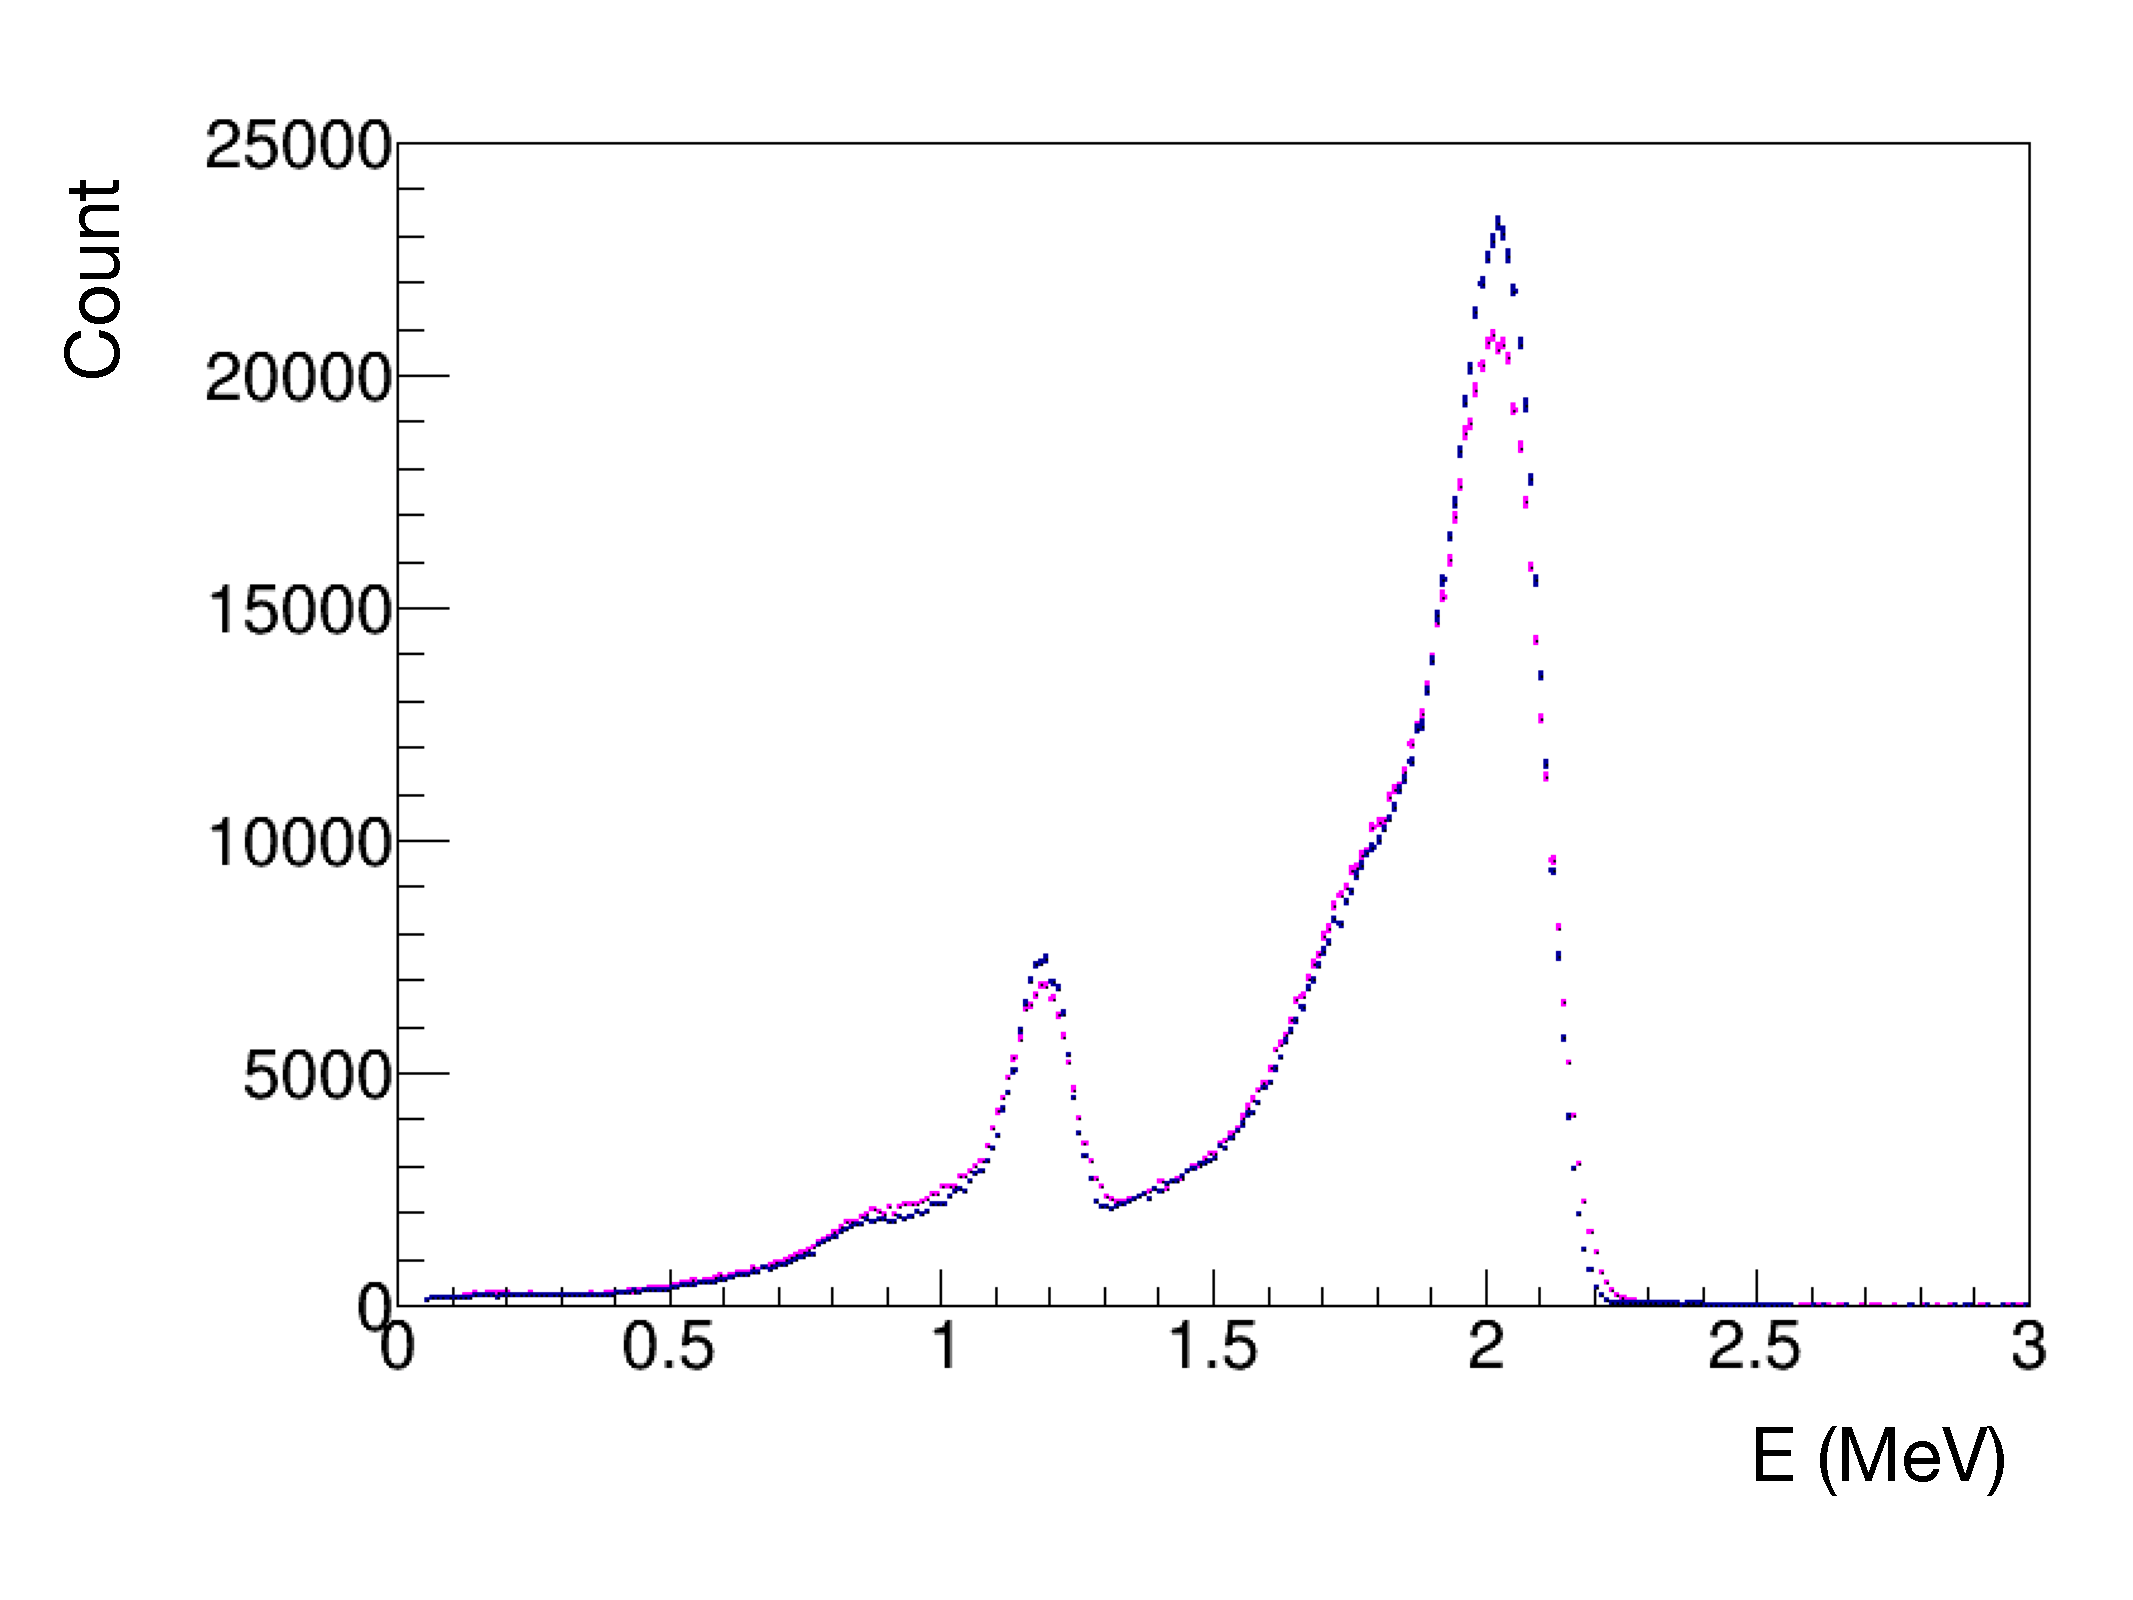
\includegraphics[width=0.7\textwidth]{Figures/Na22PG4Adjusted.pdf}
\caption[The affect of different detector parameters]{An example showing two $^{22}$Na spectra simulated with PG4 with (pink) and without (blue) detailed detector structural match.}
\label{fig:PG4geometry}
\end{figure}

Among these detector properties, the thickness of separators plays a non-negligible role in event energy loss. 
The thickness and uncertainty of the separator is $1.18 \pm 0.05$ mm, which is described in Reference \cite{bib:prospect_og}.

\begin{figure}[h!]
\centering
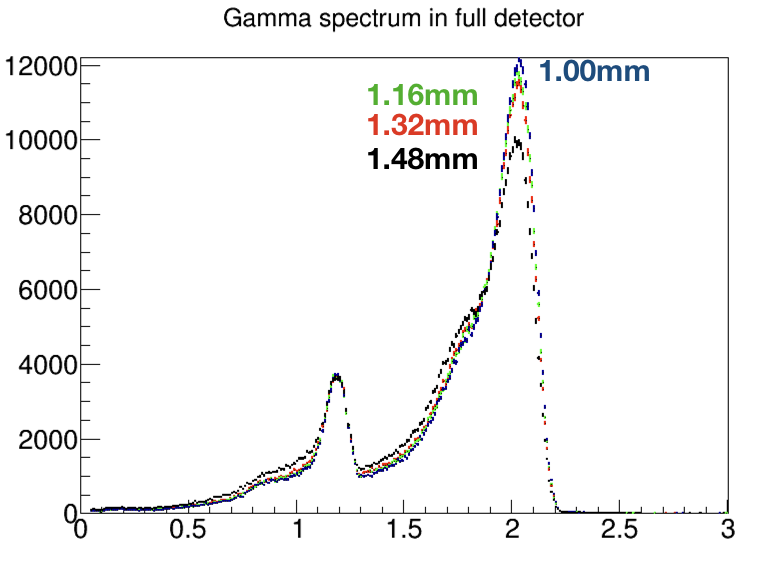
\includegraphics[width=0.7\textwidth]{Figures/thickness.png}
\caption[The affect of separator thickness to energy scale]{An example showing the thickness of separators affecting the energy loss on the spectrum.}
\label{fig:thickness}
\end{figure}

The uncertainties of the detector components' dimensions played a negligible role in energy loss. 
In Figure \ref{fig:pinwheelthick}, with exaggerated variation within $0.25$ mm, the PLA rods' wall thickness does not cause visible change to the reconstructed energy scale.

\begin{figure}[h!]
\centering
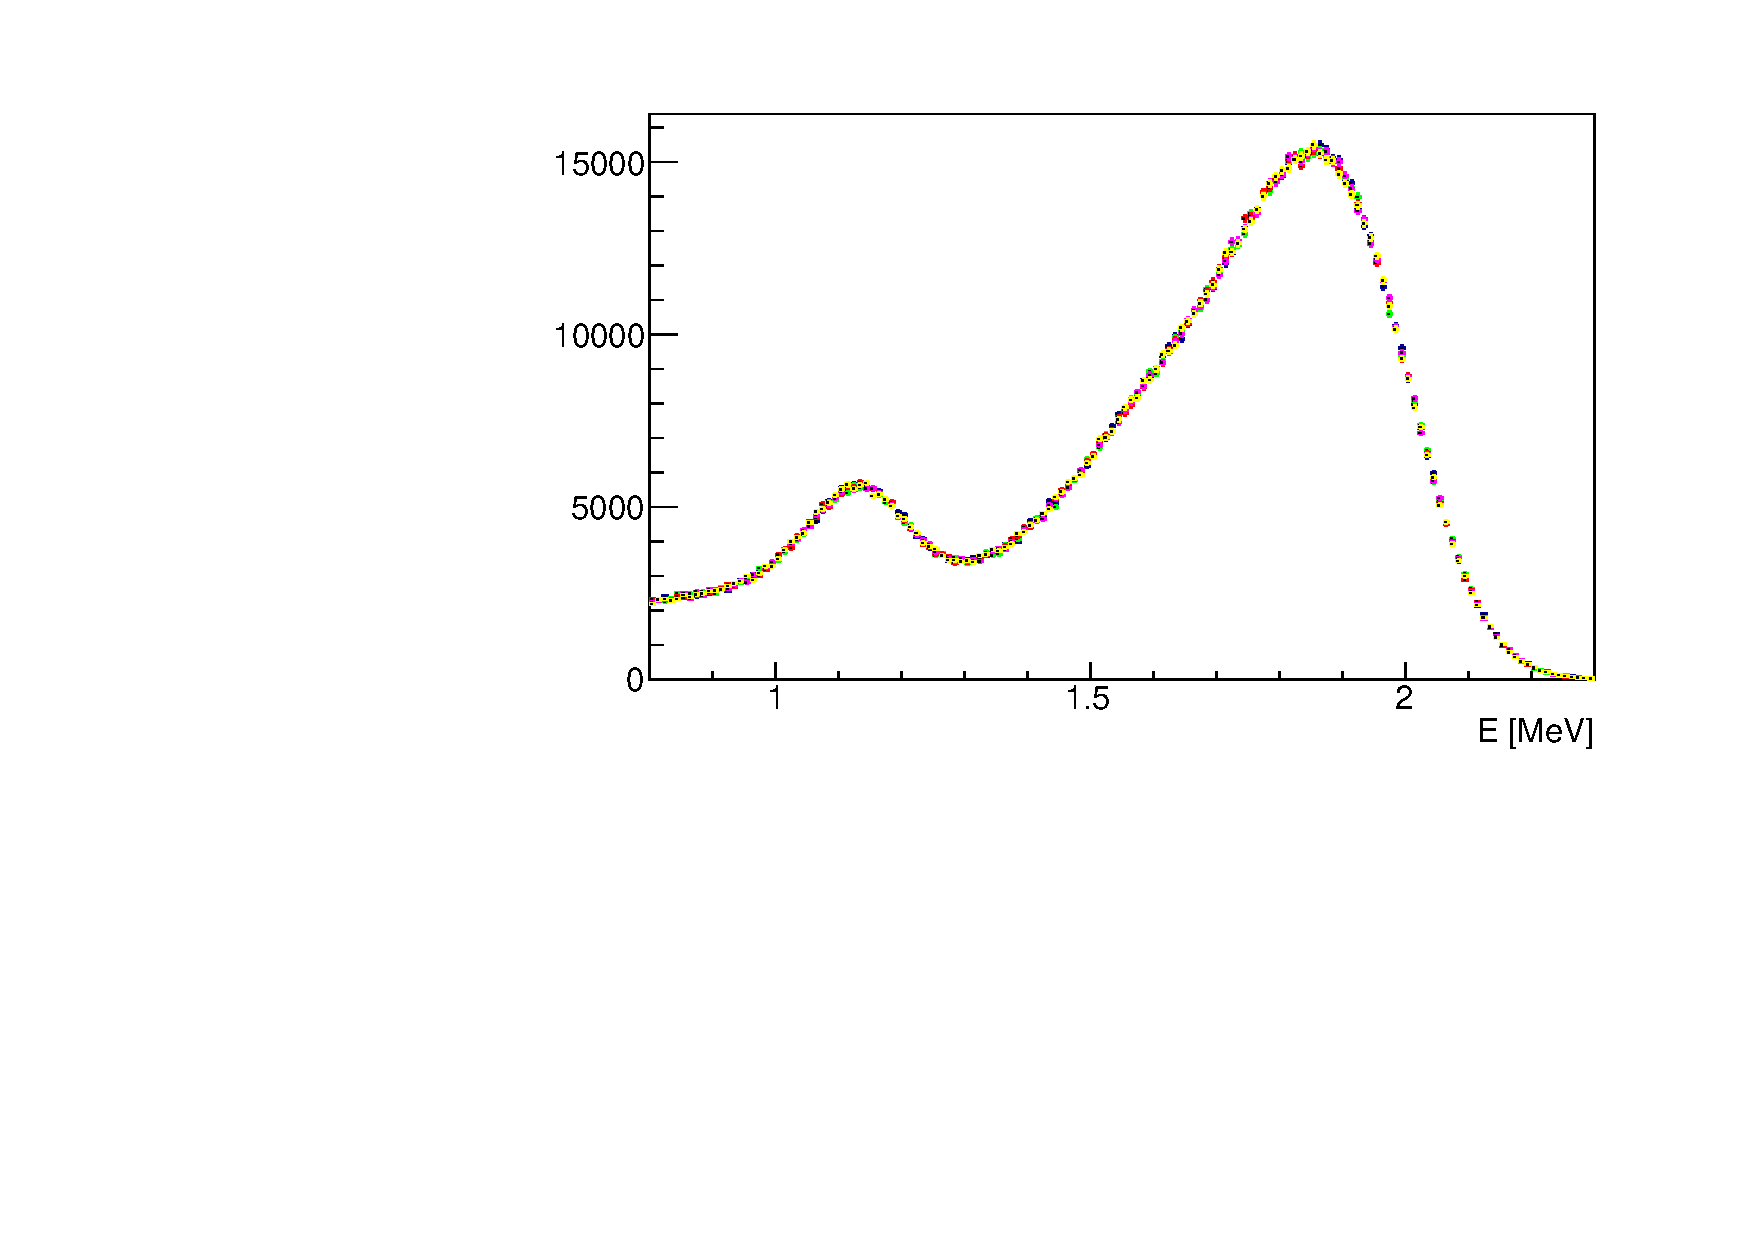
\includegraphics[width=0.7\textwidth]{Figures/pinwheelthick.pdf}
\caption[The affect of PLA rod dimensions to energy scale]{A simulated example showing the thickness of PLA rods$^\prime$ negligible effect on the energy loss. (blue: 12.1 mm; red: 12.2 mm; green: 12.3 mm; pink: 12.4 mm; yellow: 12.5 mm)}
\label{fig:pinwheelthick}
\end{figure}

\Subsection{Calibration Input Model}
The input model of radioactive calibrations was based on the decay branchings saved in the ENSDF database.
Each gamma calibration was simulated with one million decays for every nonlinearity model generated, which is comparable to the actual count of gammas produced in calibrations.
The branching information and energy levels of $^{12}$B decay are extracted from reference~\cite{bib:duke}. 
We generated 10 million $^{12}$B decays in simulation, which is considerably more statistics than data collected.
During data vs. MC comparison, the $\sim$1\% energy scale uncertainty of the $^{12}$B input spectrum was taken into consideration by pulling in the energy scale of the predicted $^{12}$B spectrum in 1\%. 
The uncertainty in $^{12}$B decay branching fractions are negligible.

Considering the gamma energy loss by the finite detector volume, the simulated calibration source location is at the same reconstructed source location from actual calibration data.

\Section{Data vs. Monte-Carlo Comparison}
\label{sec:dataMC}

The MC energy spectra and gamma multiplicities were compared to calibration data through $\chi^2$ tests. 
Calibration runs were simulated with PG4 while a variety of parameters, $k_{B1}$, $k_{B2}$ and $k_C$ were float to search for the best fit nonlinearity model, as described in section \ref{sec:nonlinear}. 
The MC files were converted to pulses and processed through a similar analysis loop as the actual calibration data, including the energy-pulse conversion described in Chapter~\ref{Ch6}.
The event based smearing and the analysis ZLE thresholds were also applied.
The data vs. MC comparison was made with a similar detector configuration, including the same dead channels, comparable event rate, and same size of fiducial volumes.
Then, the analyzed MC calibration spectra were scaled with a constant energy scale $A$.
Taking both MC's and data's statistical uncertainties into consideration, the $\chi^2$ of each comparison is expressed as:
\begin{equation}
	\chi^2 = \sum_i\frac{(O_i - WE_i)^2}{\sigma_O^2 + W^2\sigma_E^2},
\end{equation}
where $O$ and $E$ represent data and MC respectively, $W$ is the normalization factor of MC spectrum or multiplicity, and $\sigma_O$ and $\sigma_E$ are the statistical uncertainties of data and MC.
To find the best fit detector response model, the combined $\chi^2$ value is defined as
\begin{equation}
    \chi^2_{data-MC} = \sum_{\gamma} \chi^2_\gamma + \sum_{multi}\chi^2_{multi} + \chi^2_{^{12}\textrm{B}},
    \label{eq:escalechi2}
\end{equation}
where $\sum_{\gamma} \chi^2_\gamma$ is the summed $\chi^2$ of gamma energy spectra, $\sum_{multi} \chi^2_{multi}$ is the summed $\chi^2$ of gamma multiplicity, and $\chi^2_{^{12}\textrm{B}}$ is calculated by data-MC comparison of the $^{12}$B beta spectrum.
The MINUIT $\chi^2_{data-MC}$ minimization method was utilized to find the best fit four parameters. 

The $\chi^2$ value is minimized with data-MC comparison of full-detector reconstructed energy spectra and gamma multiplicity.
The best-fit model was then cross-checked with the energy measured with single detector segments that are most adjacent to the calibration sources, which is mostly affected by the LS light yield.

\Subsection{Full Detector Spectrum Comparison}
\label{sec:fulldet}
The full detector reconstructed energy spectrum is the summed energy a particle cluster. 
The energy resolution and nonlinearity affected the full detector energy spectrum not only through energy scale, but also through segment-hit multiplicity, for different quenching coefficients can reserve or reject hits through the 90~keV threshold of single cell measured energy.

To simplify the modeling of the detector response, the Birks$^\prime$ constants $k_{B1}$ and $k_{B2}$ in Eq.~\ref{eq:birkslaw} and the detection efficiency of Cherenkov photons $k_C$ were adjusted freely to search the best-fit detector response model with the data. 
Massive calibration simulations were made with 1000 combinations of $k_{B1}$, $k_{B2}$, and $k_C$.
Because of the variety of sources, each combination of parameters requires five simulations with an individual calibration source simulated.
The 1000-combination parameter search is limited by computer resources and time available.
Therefore, to search for the best fit parameters, four to five levels of narrowing down the range of the covered parameter space is necessary.
As a result, searching the best fit parameters with substantial precision took approximately 50000 computer hours. 
The final parameter search was in the range $(0.104, 0.144)$ mm/MeV for $k_{B1}$ with 0.004 mm/MeV steps, $(0.0011, 0.051)$ mm/MeV for $k_{B2}$ with 0.004 mm/MeV steps and $(29, 49)\%$ for $k_C$ with $2\%$ steps. 

For the efficiency of massive comparisons, the range of gamma spectrum comparison were defined automatically in software. 
A custom program was used to search Gaussian-like distributions in the energy spectrum.
The range of the fitting is the $3\sigma$ range of the tagged peaks.
In the case of $^{22}$Na calibration, where the distribution contains two peaks, the range is from the lower limit of the lower energy peak and the upper limit of the higher energy peak.
For multiplicity, the range of comparison is from 1 to 10.
For $^{12}$B comparison, the range of fitting is 3~MeV to 13.5~MeV.

Figure~\ref{fig:goodfit2} shows the full detector calibration spectra comparison best-fit model, where $\chi^2/NDF = 581.5/420$ with the parameters: $k_{B1} = 0.132 \pm 0.004$ mm/MeV, $k_{B2} = 0.023 \pm 0.004$ mm/MeV $k_C = 37 \pm 2\%$, with an absolute energy scale of $A = 100.26\pm0.46\%$. 
There were $\chi^2/NDF = 205.9/60$ contributed by the multiplicity fitting.
The data-MC energy spectra comparison of the best-fit model is shown in Figure \ref{fig:goodfit2}, and the multiplicity comparison is shown in Figure~\ref{fig:multi}.

\begin{figure}[h!]
\centering
\subfigure[]{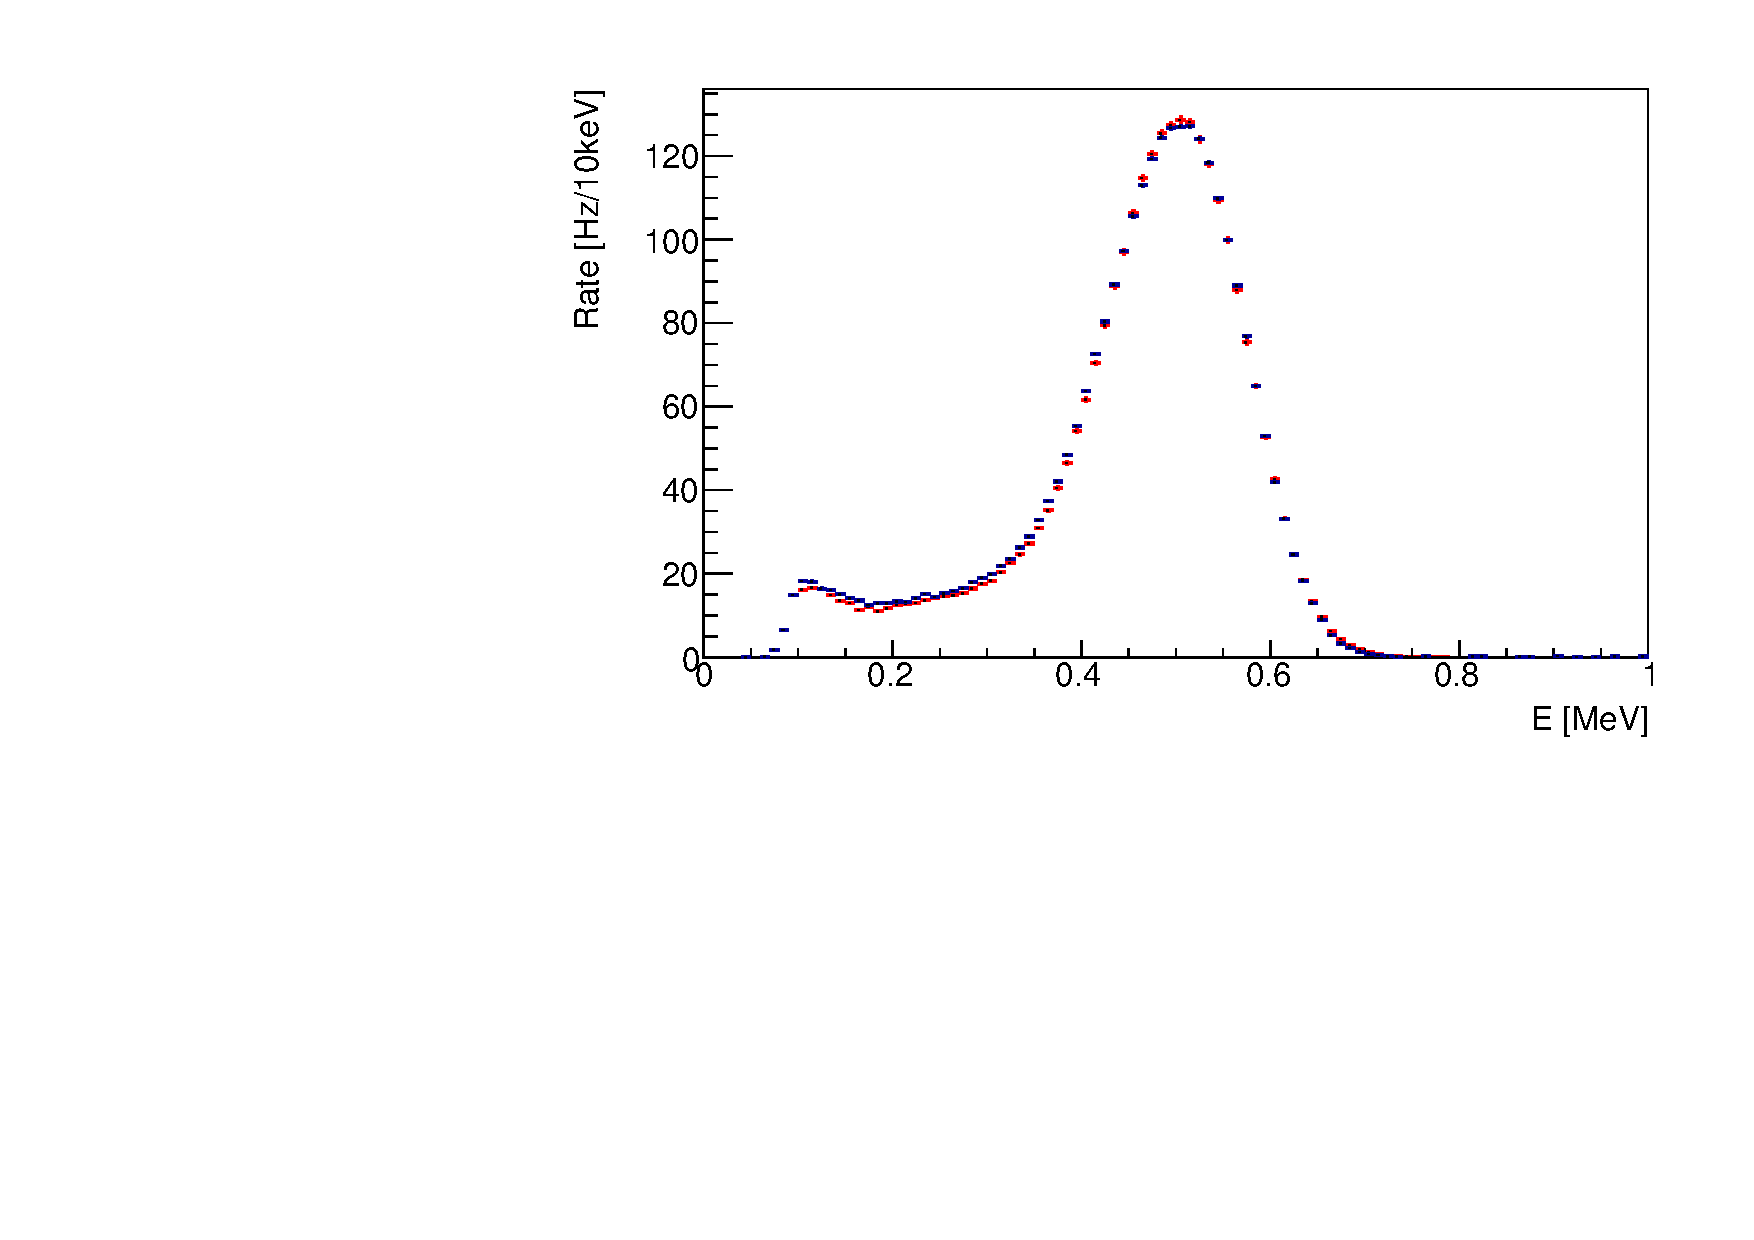
\includegraphics[width=0.45\textwidth]{Figures/hCs137v2.pdf}}\quad
\subfigure[]{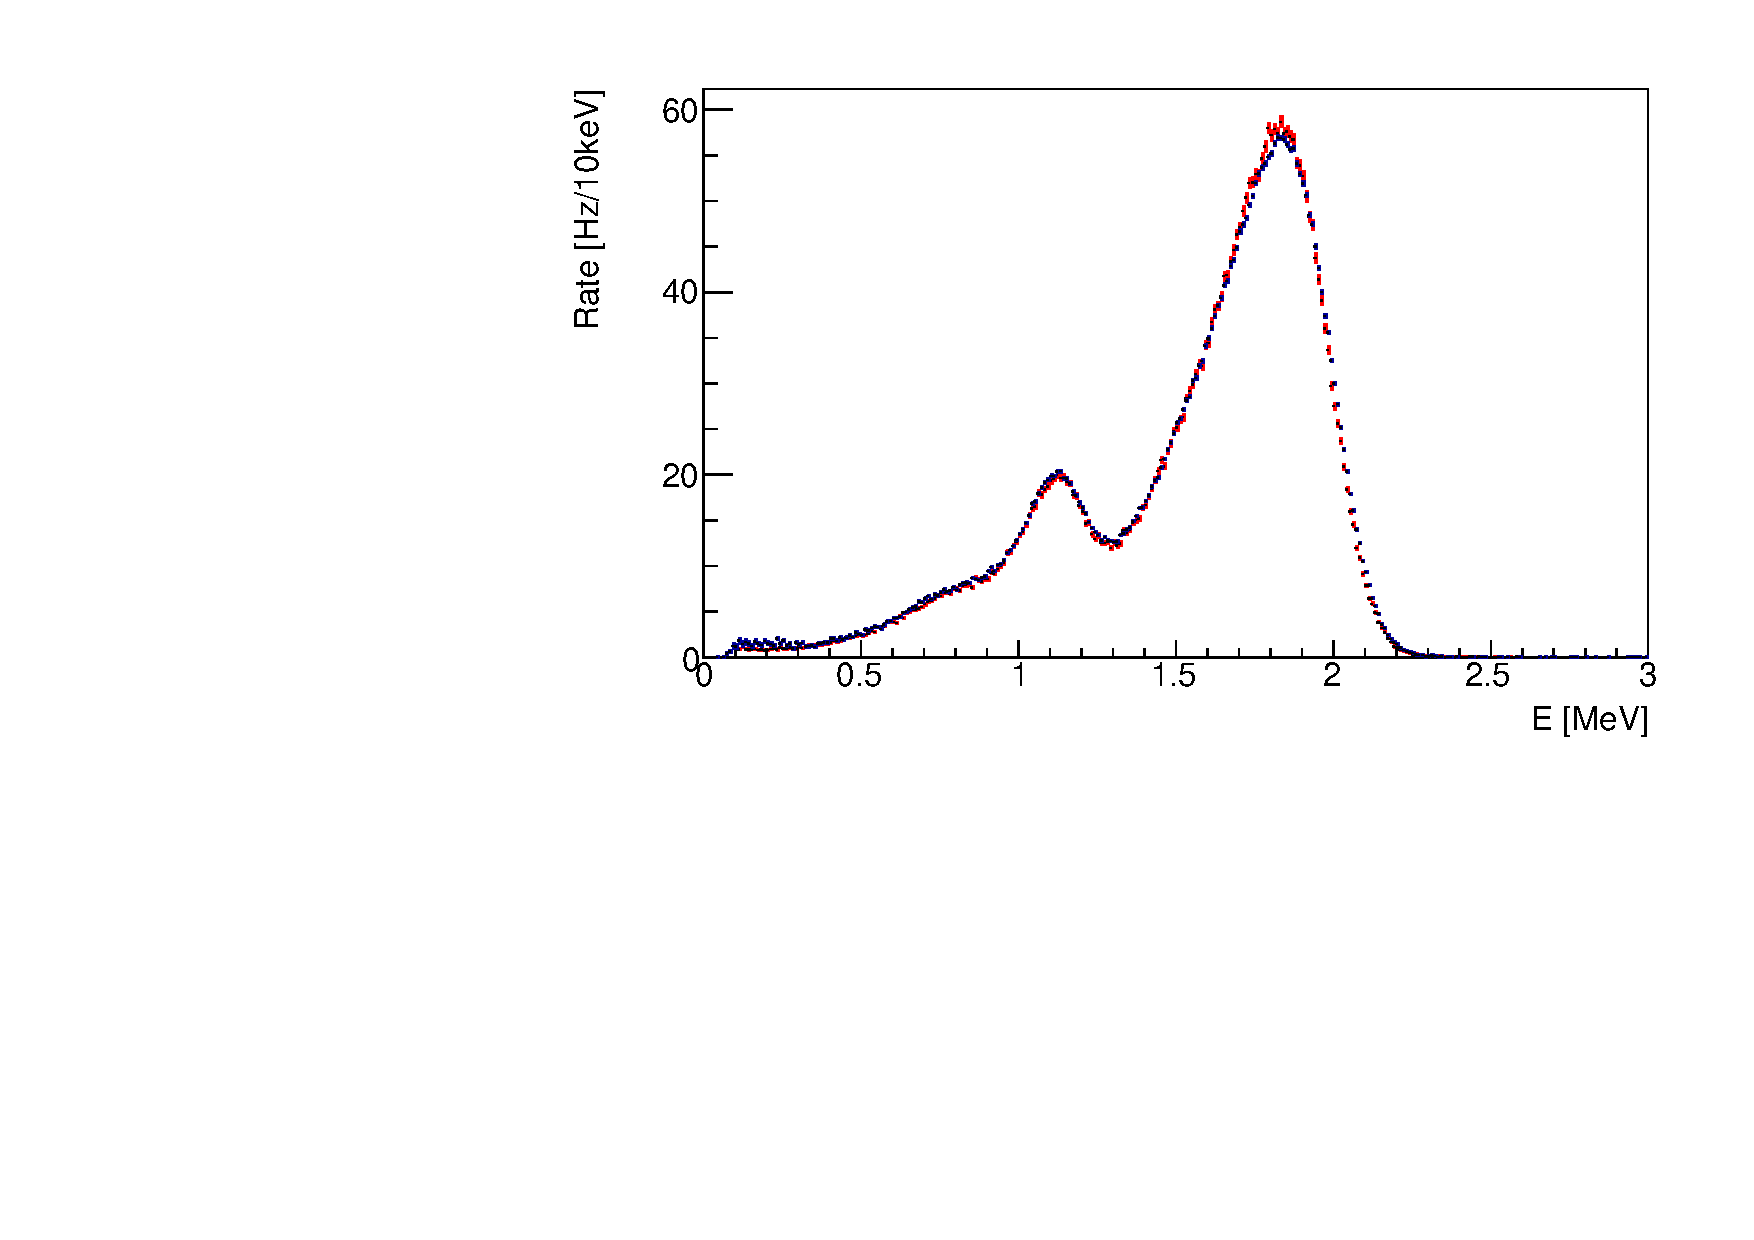
\includegraphics[width=0.45\textwidth]{Figures/hNa22v2.pdf}} \\
\subfigure[]{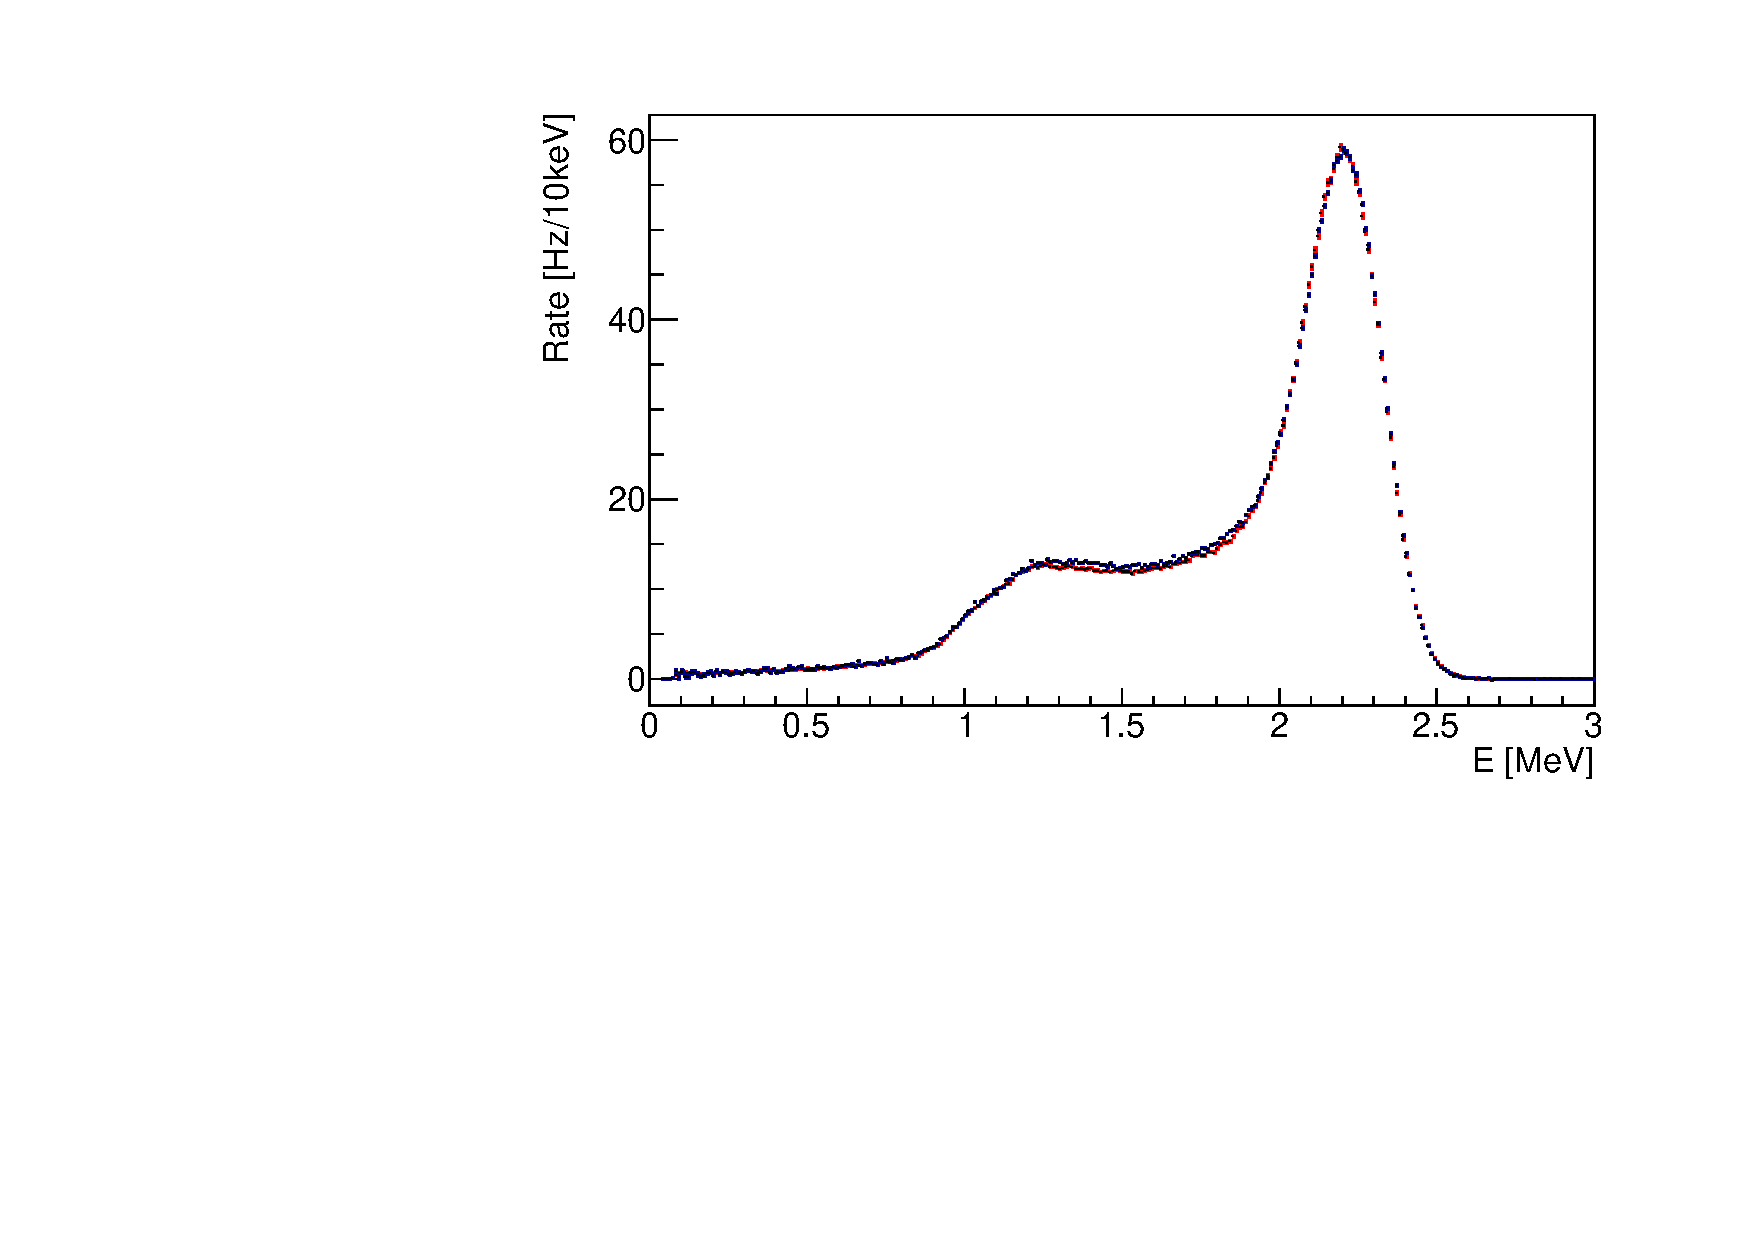
\includegraphics[width=0.45\textwidth]{Figures/hCo60v2.pdf}} \quad
\subfigure[]{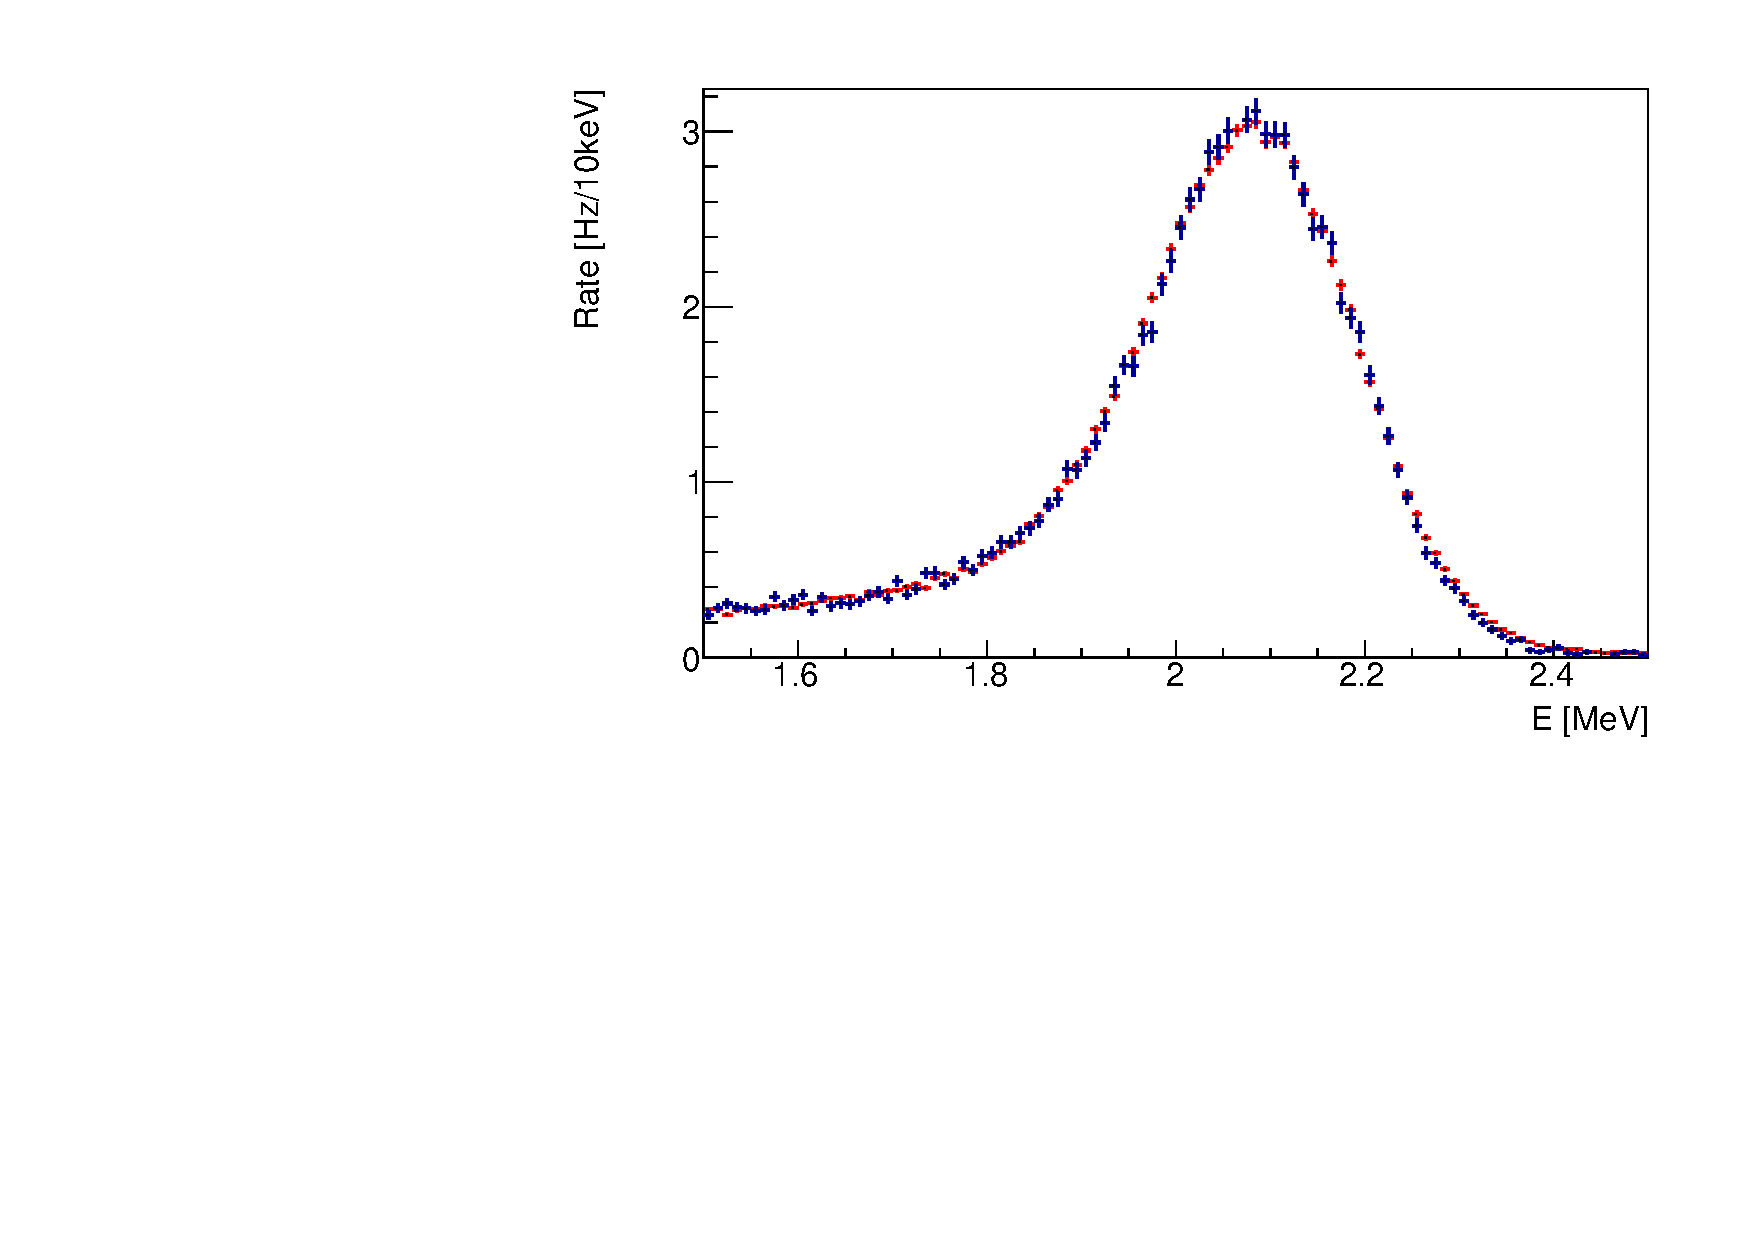
\includegraphics[width=0.45\textwidth]{Figures/hCf252v2.pdf}} \\
\subfigure[Full detector MC-data for $^{12}$B spectrum.]{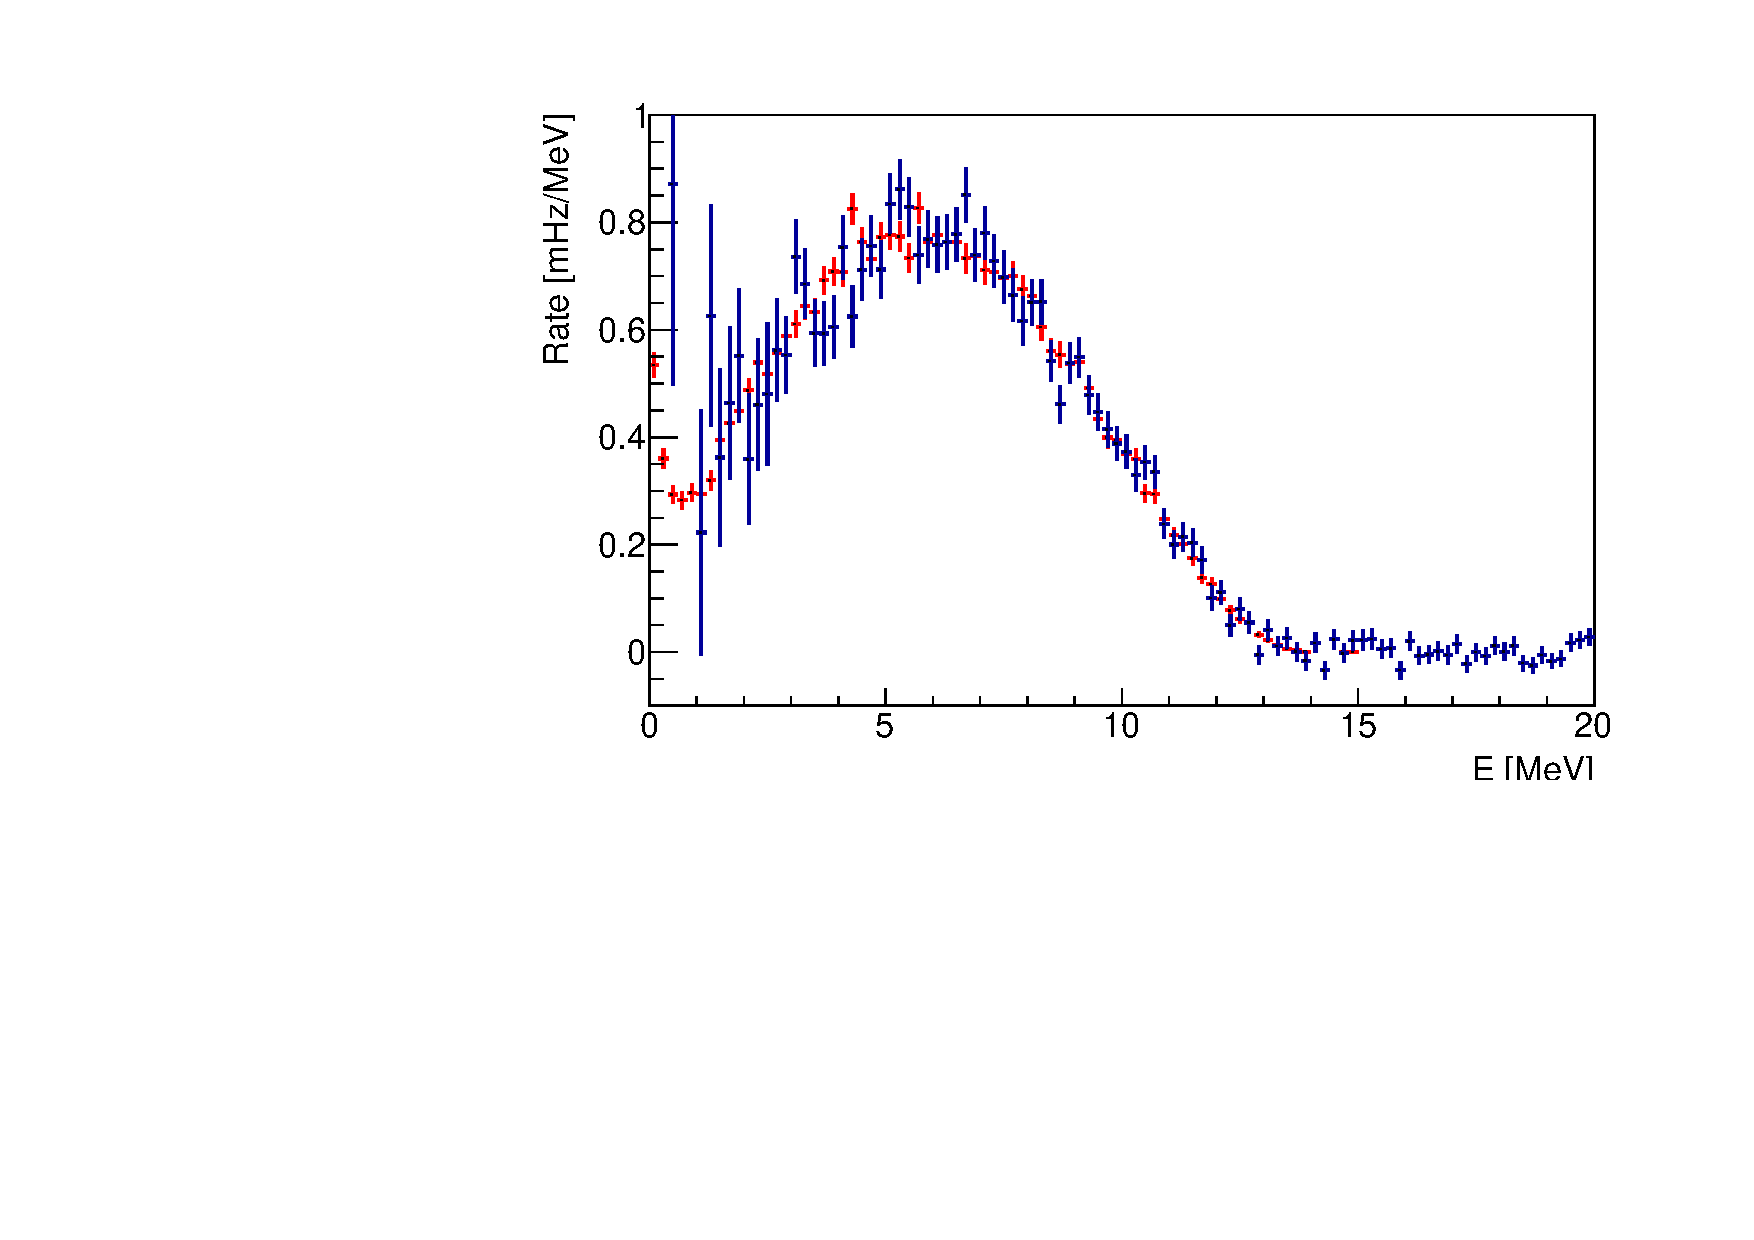
\includegraphics[width=0.45\textwidth]{Figures/hB12v2.pdf}}
\caption[Full detector data to MC gamma energy comparisons]{The full detector calibration energy spectra data vs. MC. comparison, with statistical errors only. (red: MC, blue: data) (a) $^{137}$Cs, (b) $^{22}$Na, (c) $^{60}$Co, (d) $n$-H capture gamma from $^{252}$Cf.}
\label{fig:goodfit2}
\end{figure}

\begin{figure}[h!]
\centering
\subfigure[]{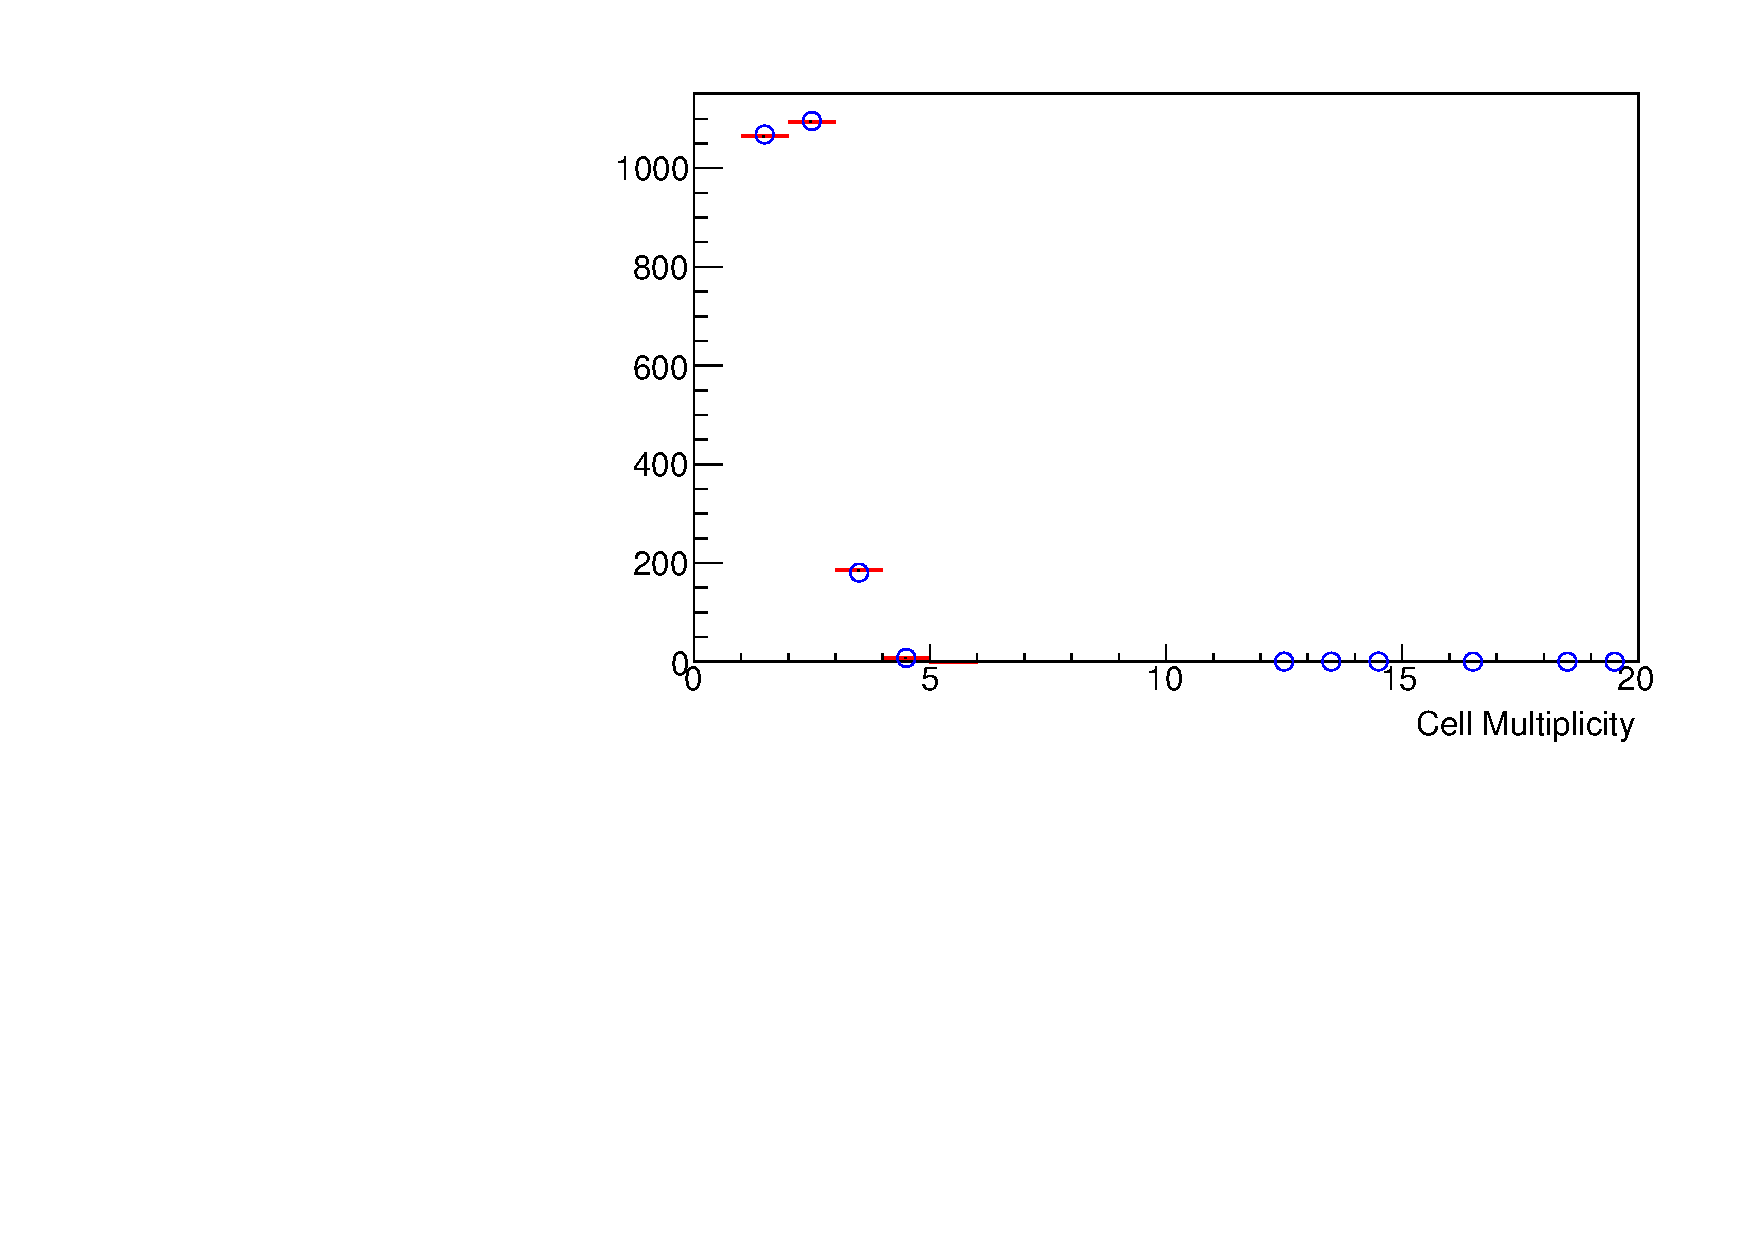
\includegraphics[width=0.45\textwidth]{Figures/hCs137multi.pdf}}\quad
\subfigure[]{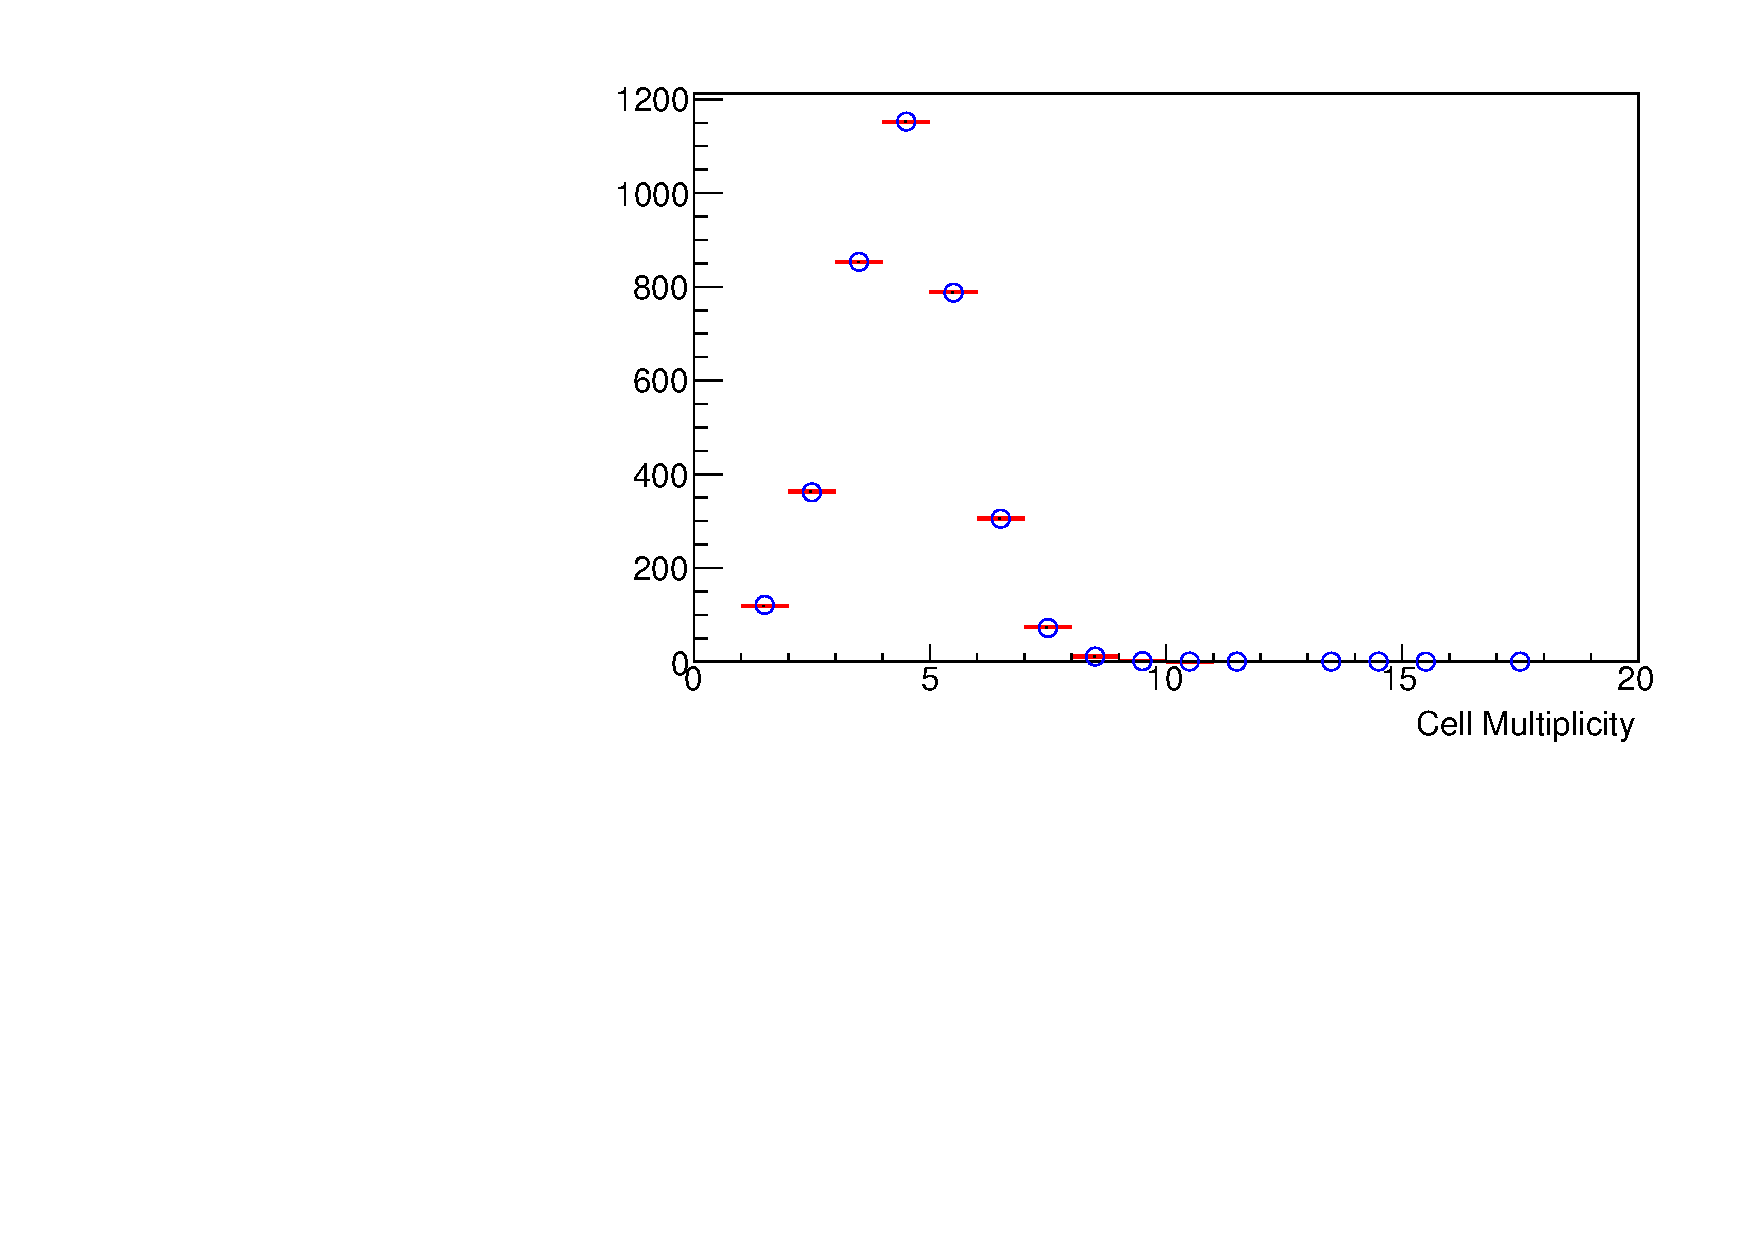
\includegraphics[width=0.45\textwidth]{Figures/hNa22mulit.pdf}} \\
\subfigure[]{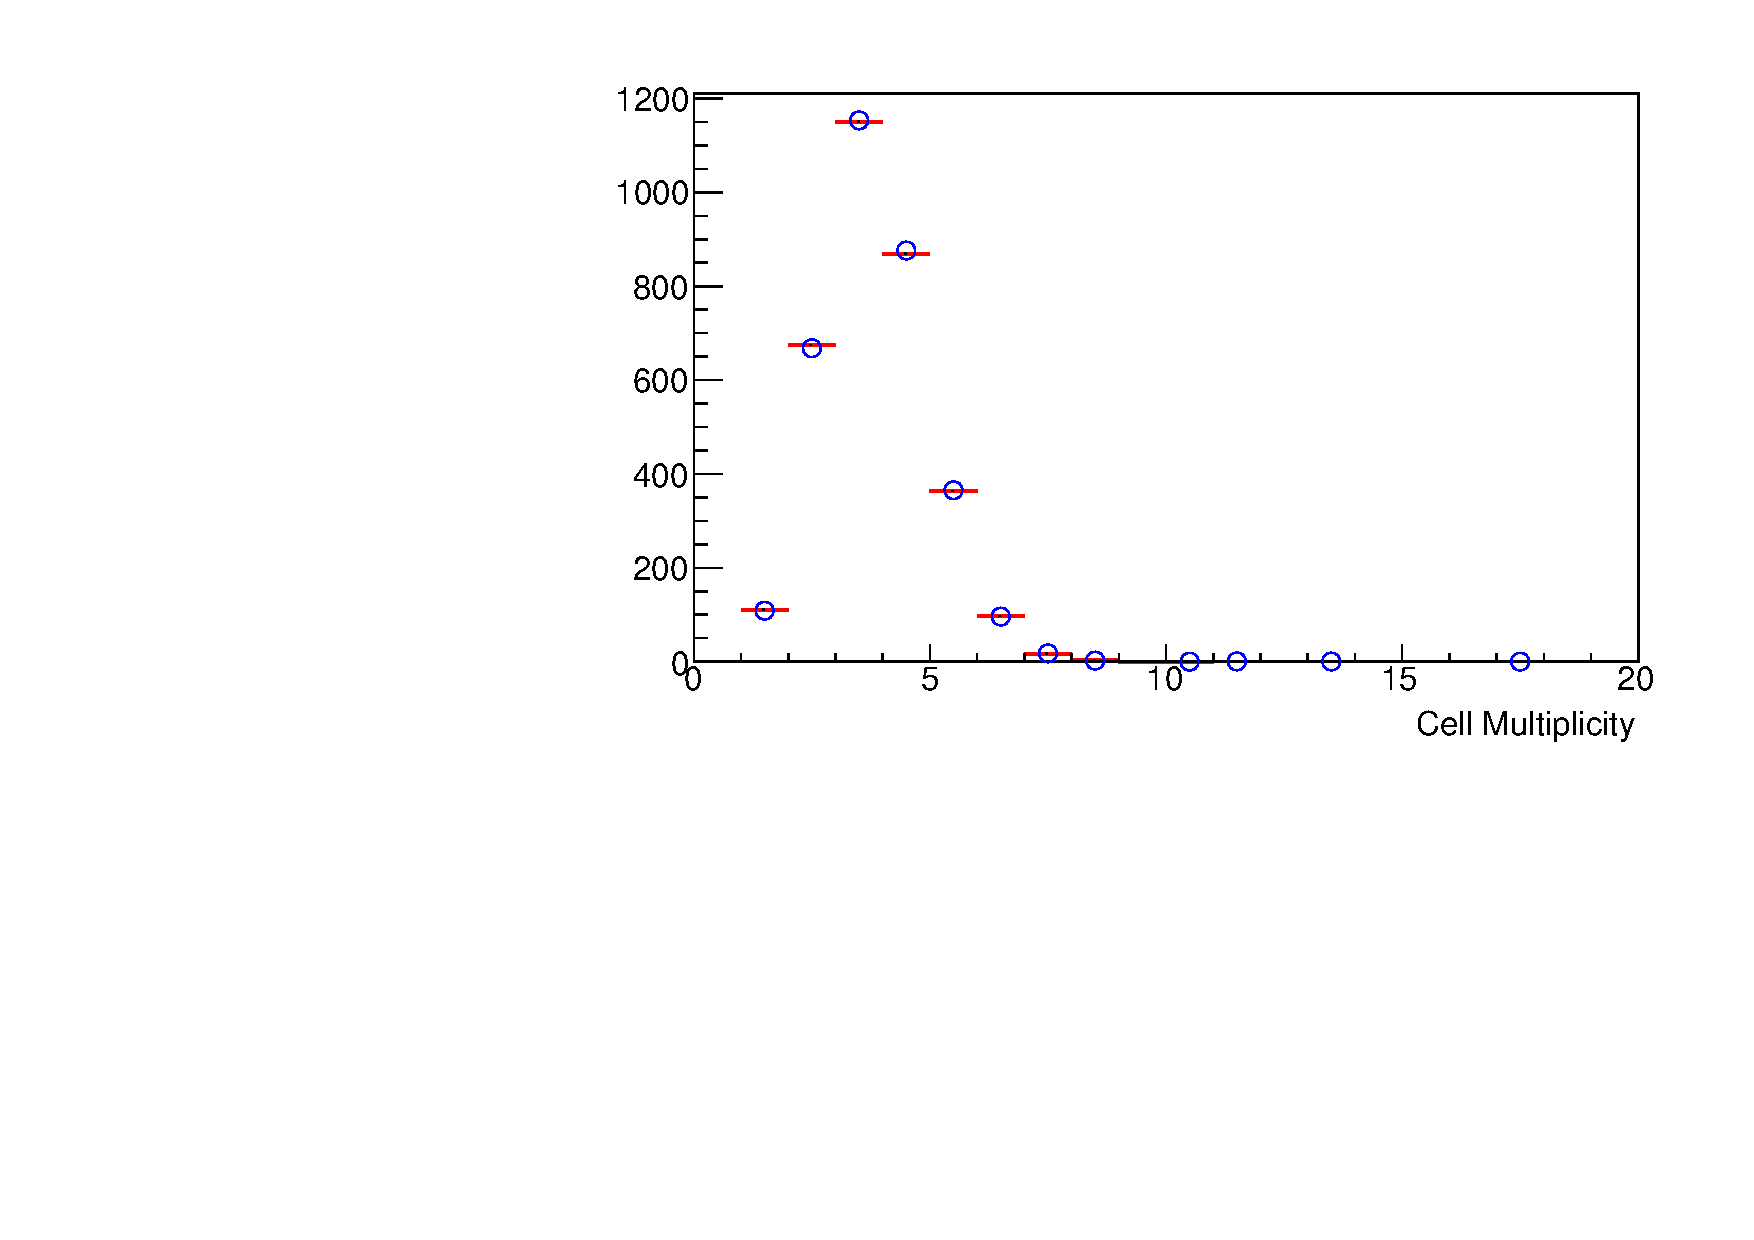
\includegraphics[width=0.45\textwidth]{Figures/hCo60multi.pdf}} 
\subfigure[]{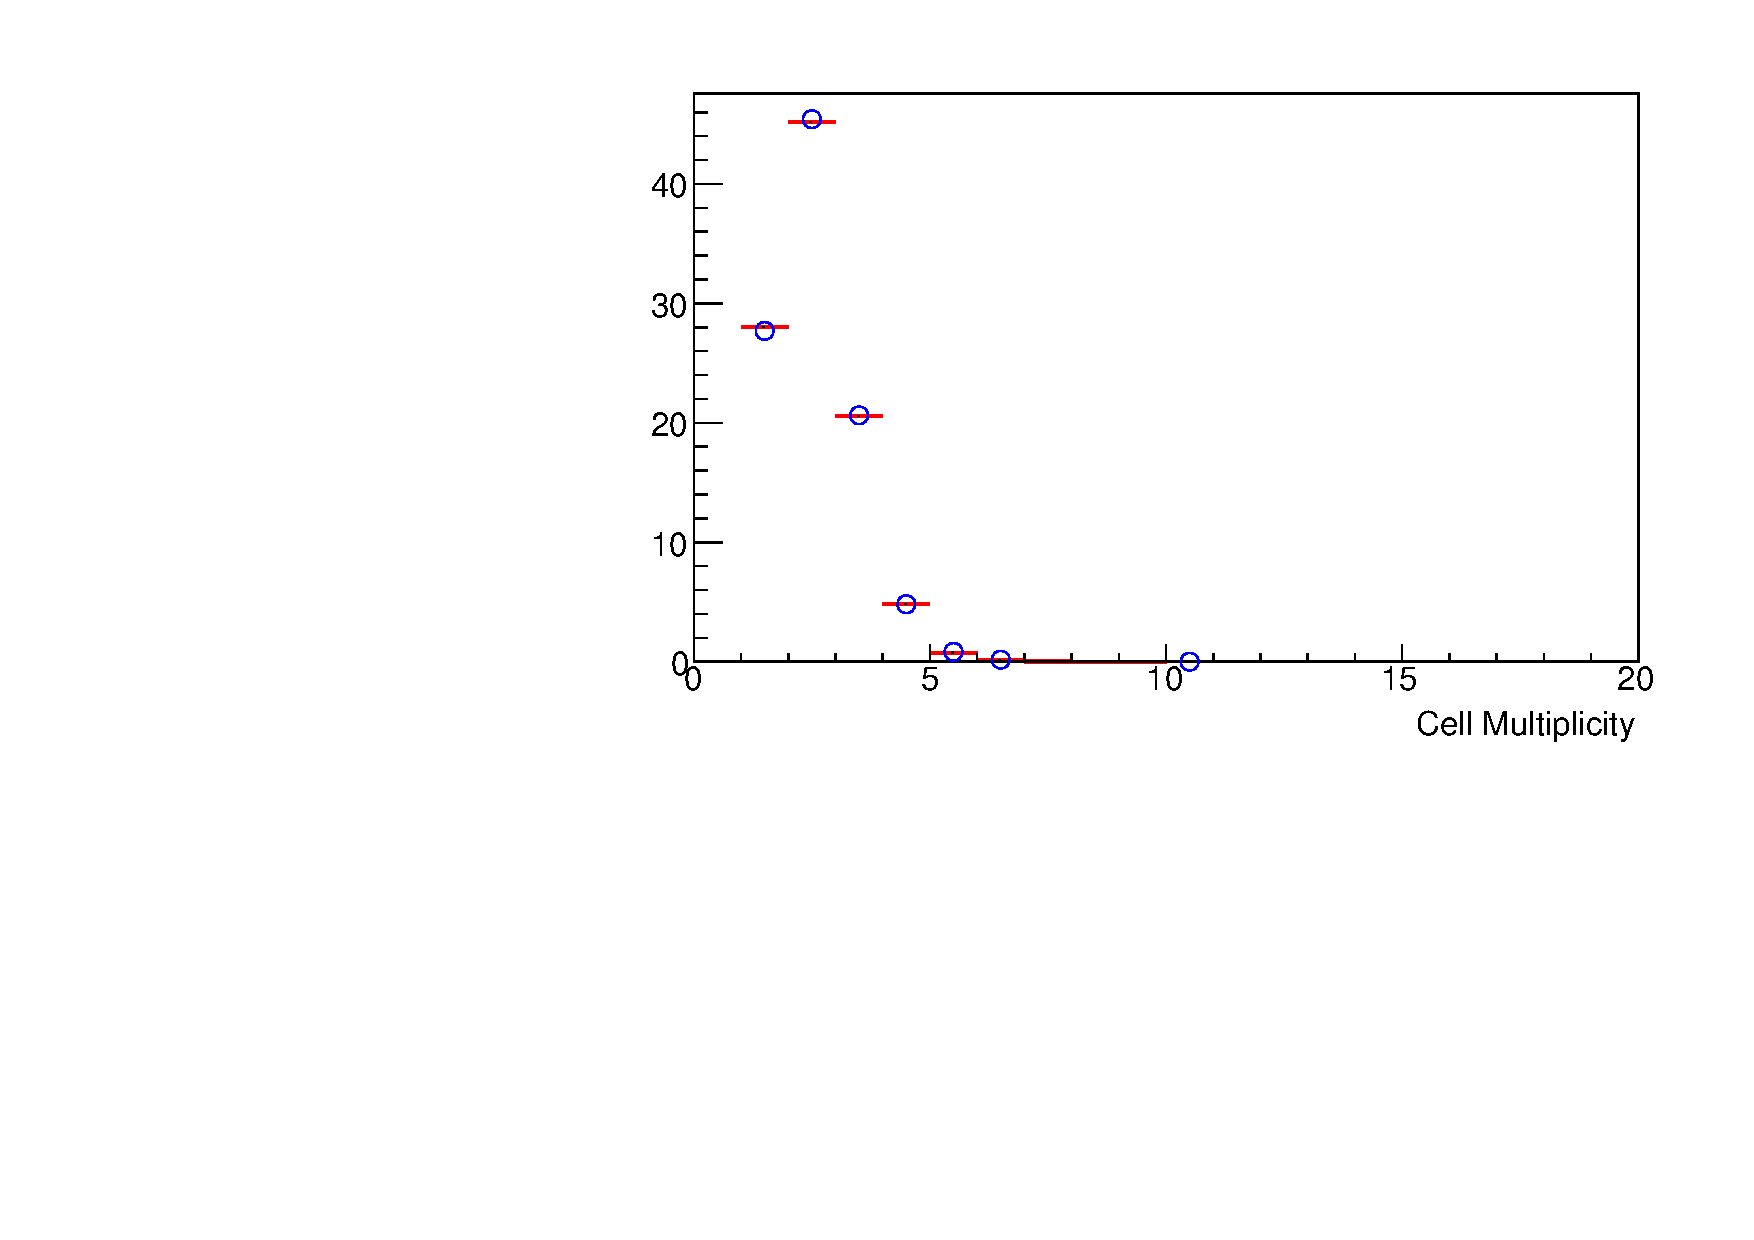
\includegraphics[width=0.45\textwidth]{Figures/hCf252multi.pdf}} 
\caption[Full detector data vs MC gamma multiplicity comparisons]{Data vs. MC comparisons multiplicity distributions of gamma calibrations. (red: MC, blue: Data) (a) $^{137}$Cs, (b) $^{22}$Na, (c) $^{60}$Co, (d) $n$-H capture gamma from $^{252}$Cf.}
\label{fig:multi}
\end{figure}

The $\chi^2$ distributions dependent on combinations of $k_{B1}$ and $k_{B2}$, $k_{B1}$ and $k_{C}$, and $k_{B2}$ and $k_{C}$ are shown in Figure \ref{fig:chi2}.
The nonlinearity parameters shown are correlated.
At this current stage, the correlations among the parameters is not studied.
As a result, the uncertainty calculated covers all parameter sets in the 1-$\sigma$ range of each individual parameter.

\begin{figure}[h!]
\centering
\subfigure[]{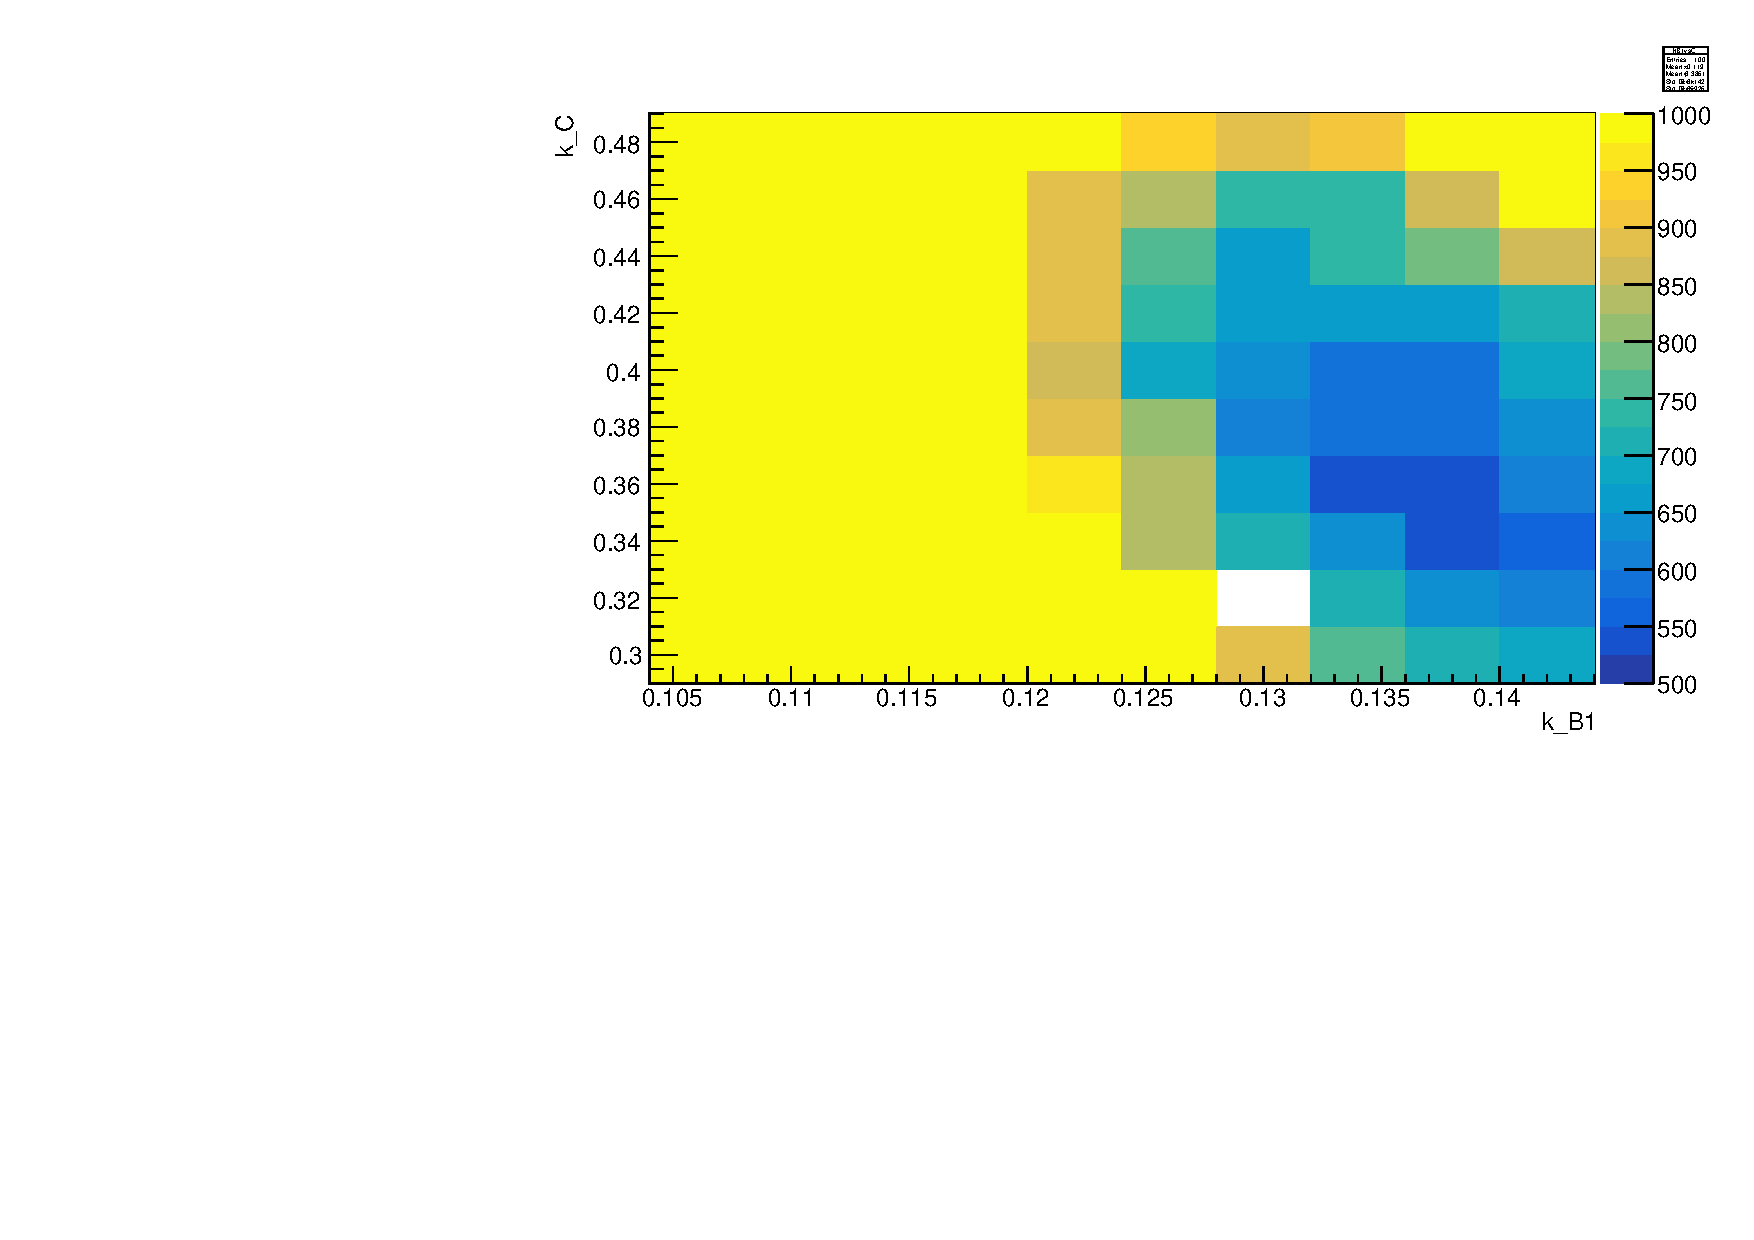
\includegraphics[width=70mm]{Figures/k1vkc.pdf}}\quad
\subfigure[]{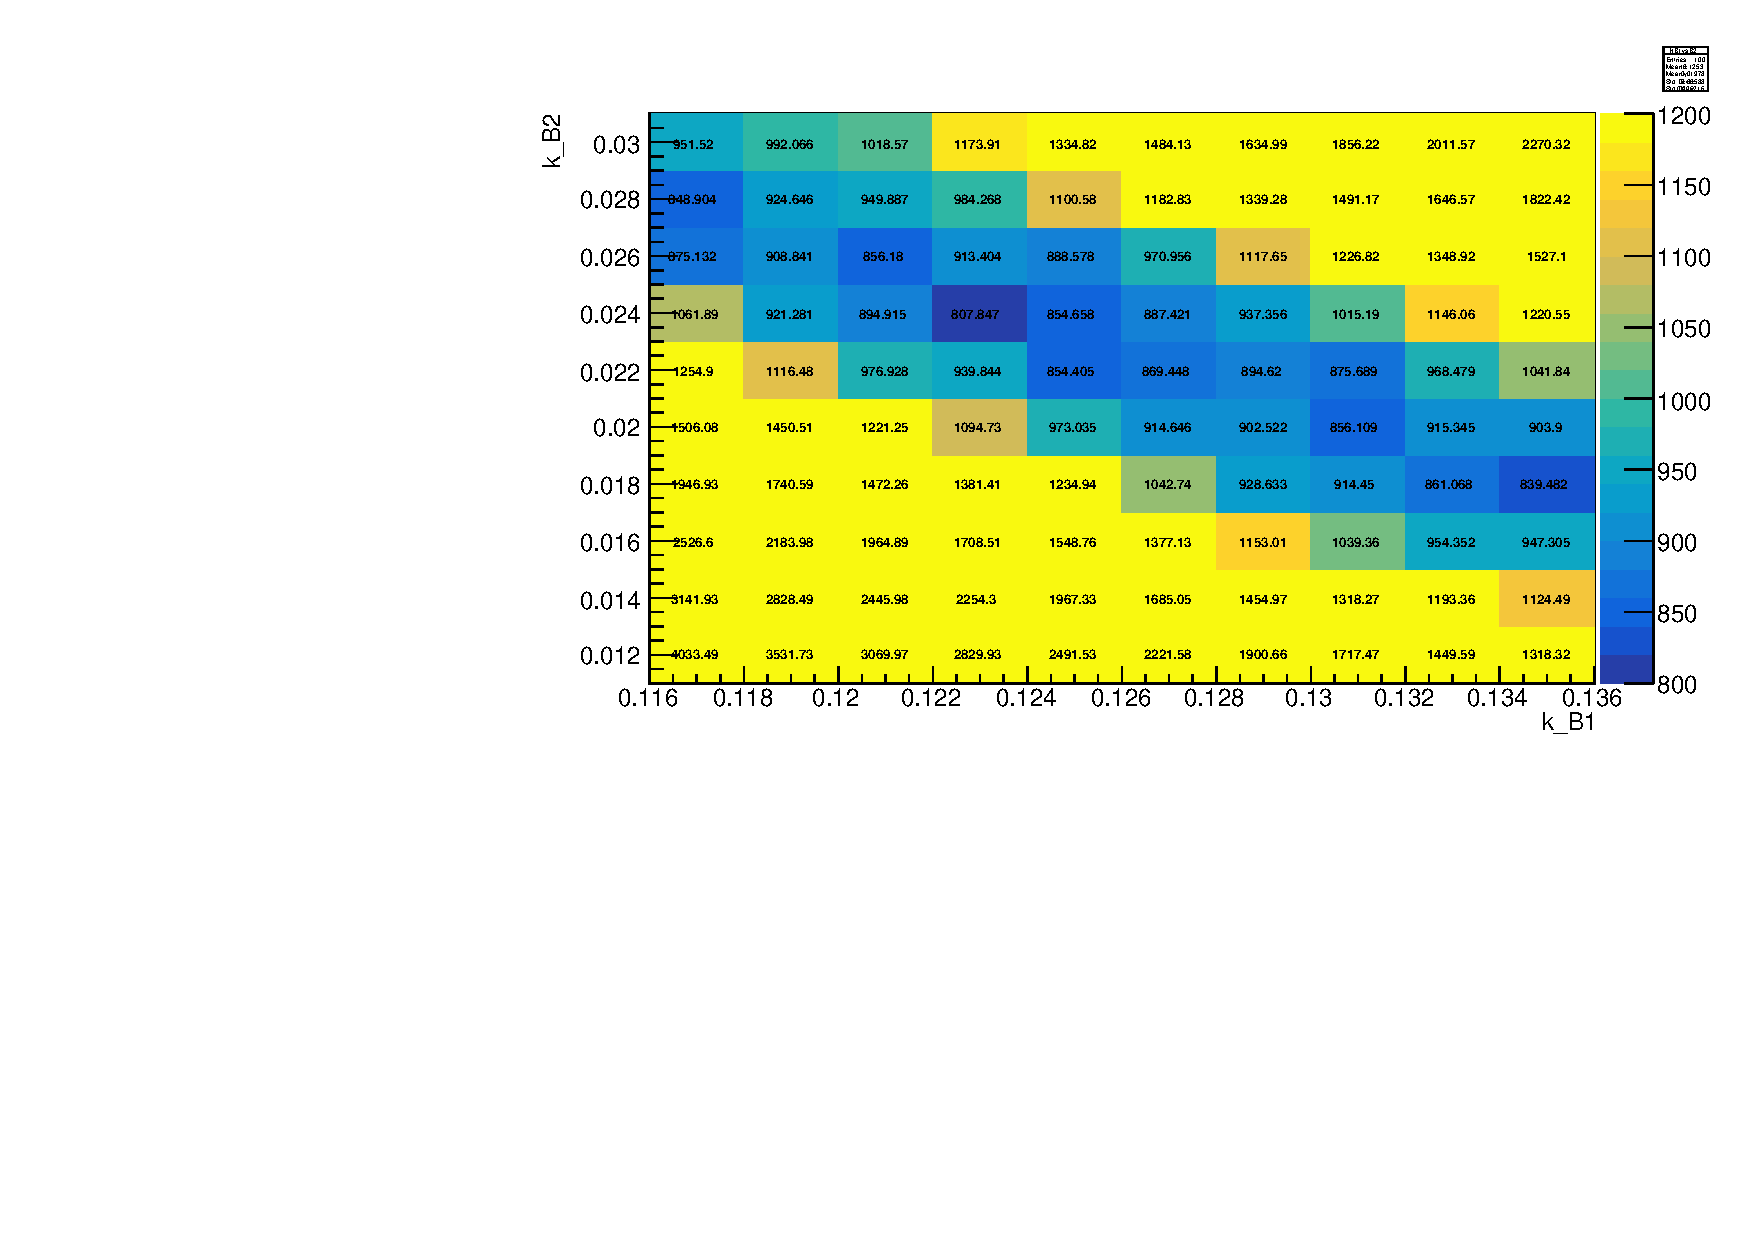
\includegraphics[width=70mm]{Figures/k1vk2.pdf}} \\
\subfigure[]{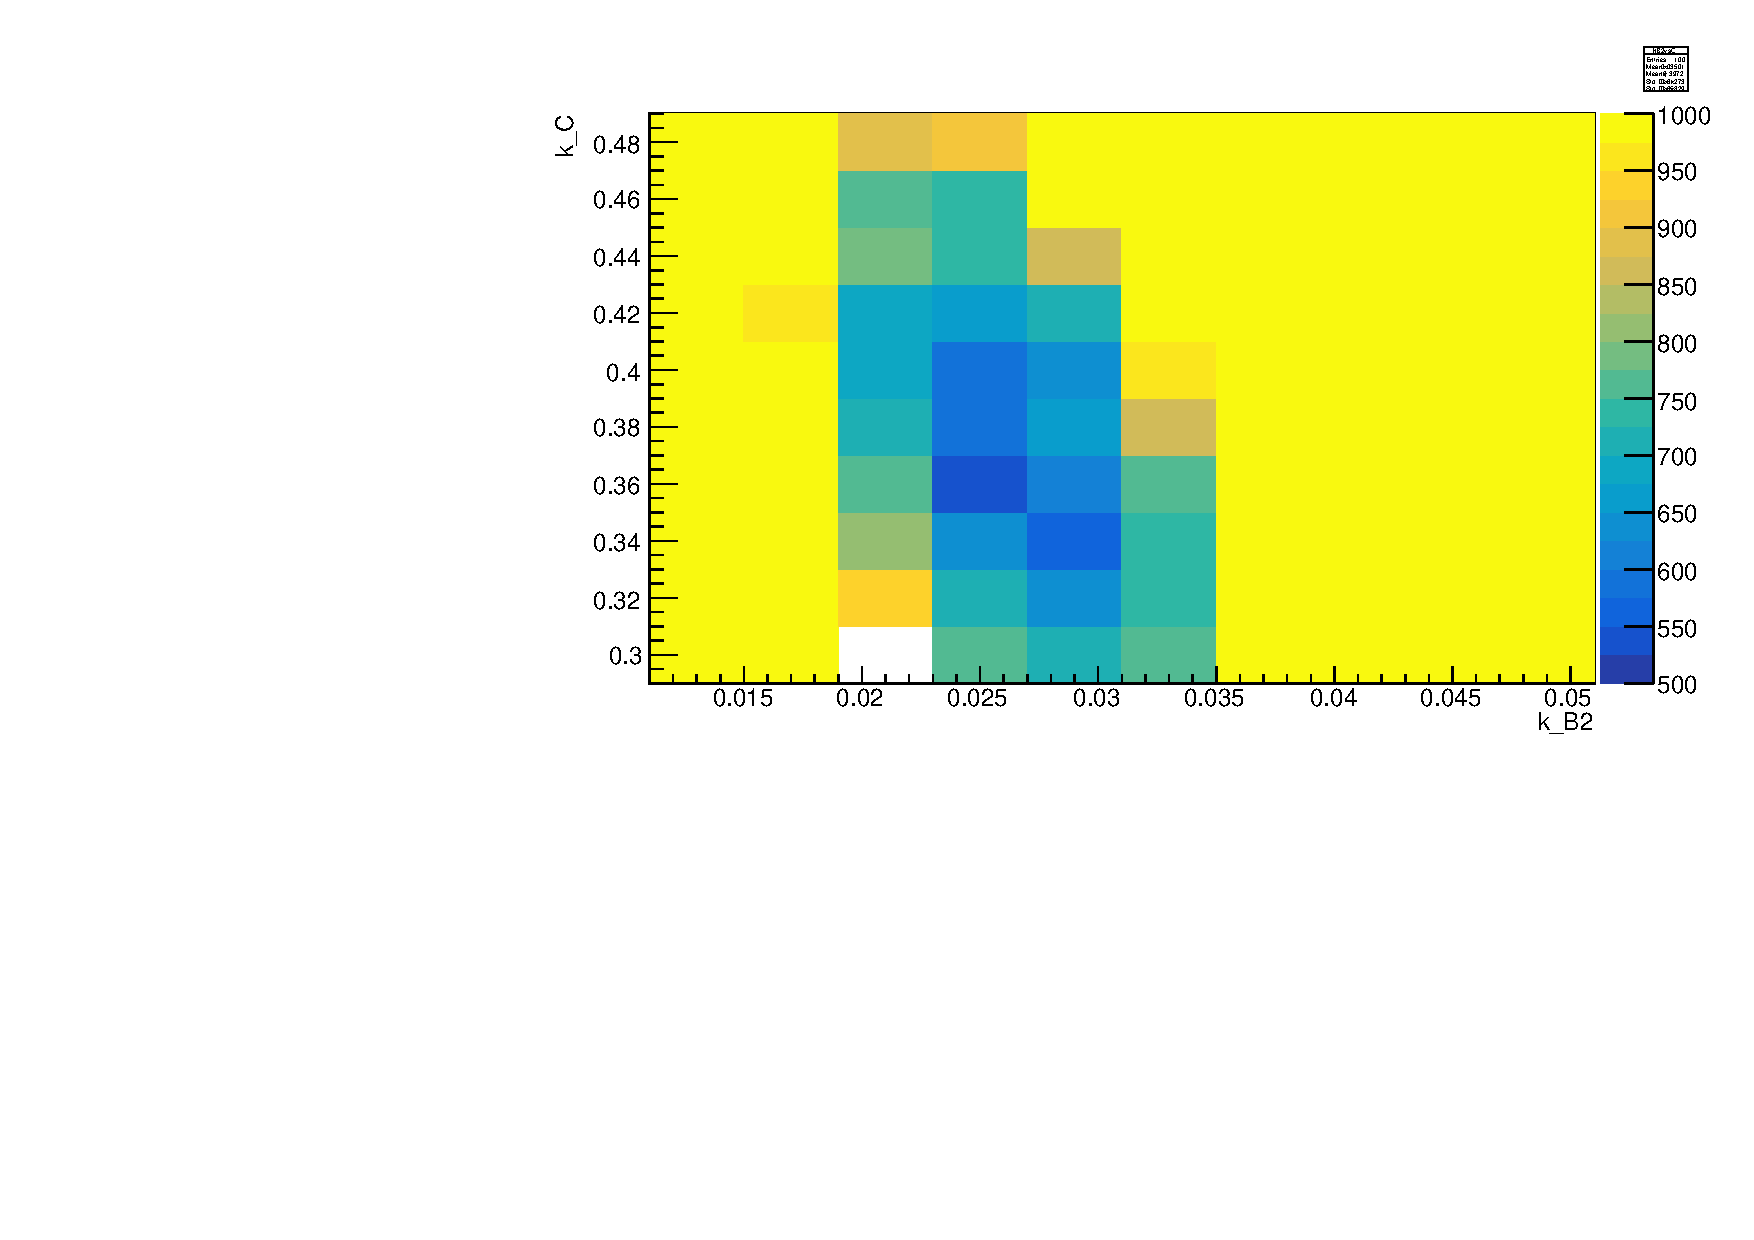
\includegraphics[width=70mm]{Figures/k2vkc.pdf}} 
\caption[$\chi^2$ distributions with respect to the values of nonlinearity parameters.]{$\chi^2$ distribution with respect to the values of the nonlinearity parameters.
(a) $\chi^2$ distribution dependent on $k_{B1}$ and $k_{C}$.
(b) $\chi^2$ distribution dependent on $k_{B1}$ and $k_{B2}$.
(c) $\chi^2$ distribution dependent on $k_{B2}$ and $k_{C}$.}
\label{fig:chi2}
\end{figure}
\newpage
\clearpage

\Subsection{Single Cell Spectrum Comparison}
\label{sec:single}
The calibration energy spectra measured by single segments of the PROSPECT AD are independent from the energy loss caused by detector dead volume and the analysis ZLE threshold's low energy hit exclusion.
The data and MC agreement in single-segment reconstructed energy is a valuable cross-check to the full-detector best fit model.
The cross-check is to compare the reconstructed and simulated Compton scattering energy spectrum measured by the single segments that are most adjacent to the calibration sources.

Each source has four most adjacent segments.
To reduce the systematic differences of energy scale between segments, the gamma spectra from four segments were averaged. 
For gamma radioactive calibrations, the range of fitting is from 0.3 MeV to the ends of the spectra.
The range of fitting of the gamma spectrum from n-H capture was 1.5 MeV to 2.3 MeV.
In single cell comparison, we compare only the single hit $^{12}$B electron energy spectrum.
The range of fitting for the $^{12}$B spectrum is 3 to 13.5 MeV. 
To simplify the fitting, the MC spectra were normalized to data based on the spectral integral in the range of interest.
$\chi^2$ comparison of each calibration spectrum was made between data and a best fit MC. 
Then, the summed $\chi^2$ of all comparisons was evaluated.

The data vs. MC comparisons with full detector best fits are shown in Figure \ref{fig:goodfit}. 
The summed $\chi^2/NDF = 1003.29/584$ with the parameters of the nonlinearity model obtained in the full-detector fitting in Section \ref{sec:fulldet}.
The average energy shift is $A=100.30\%$.
The single segment data vs. MC comparison demonstrated the best fit energy scale factors are compatible with the single LS volume reconstructed Compton scattering energy.

\begin{figure}[h!]
\centering
\subfigure[]{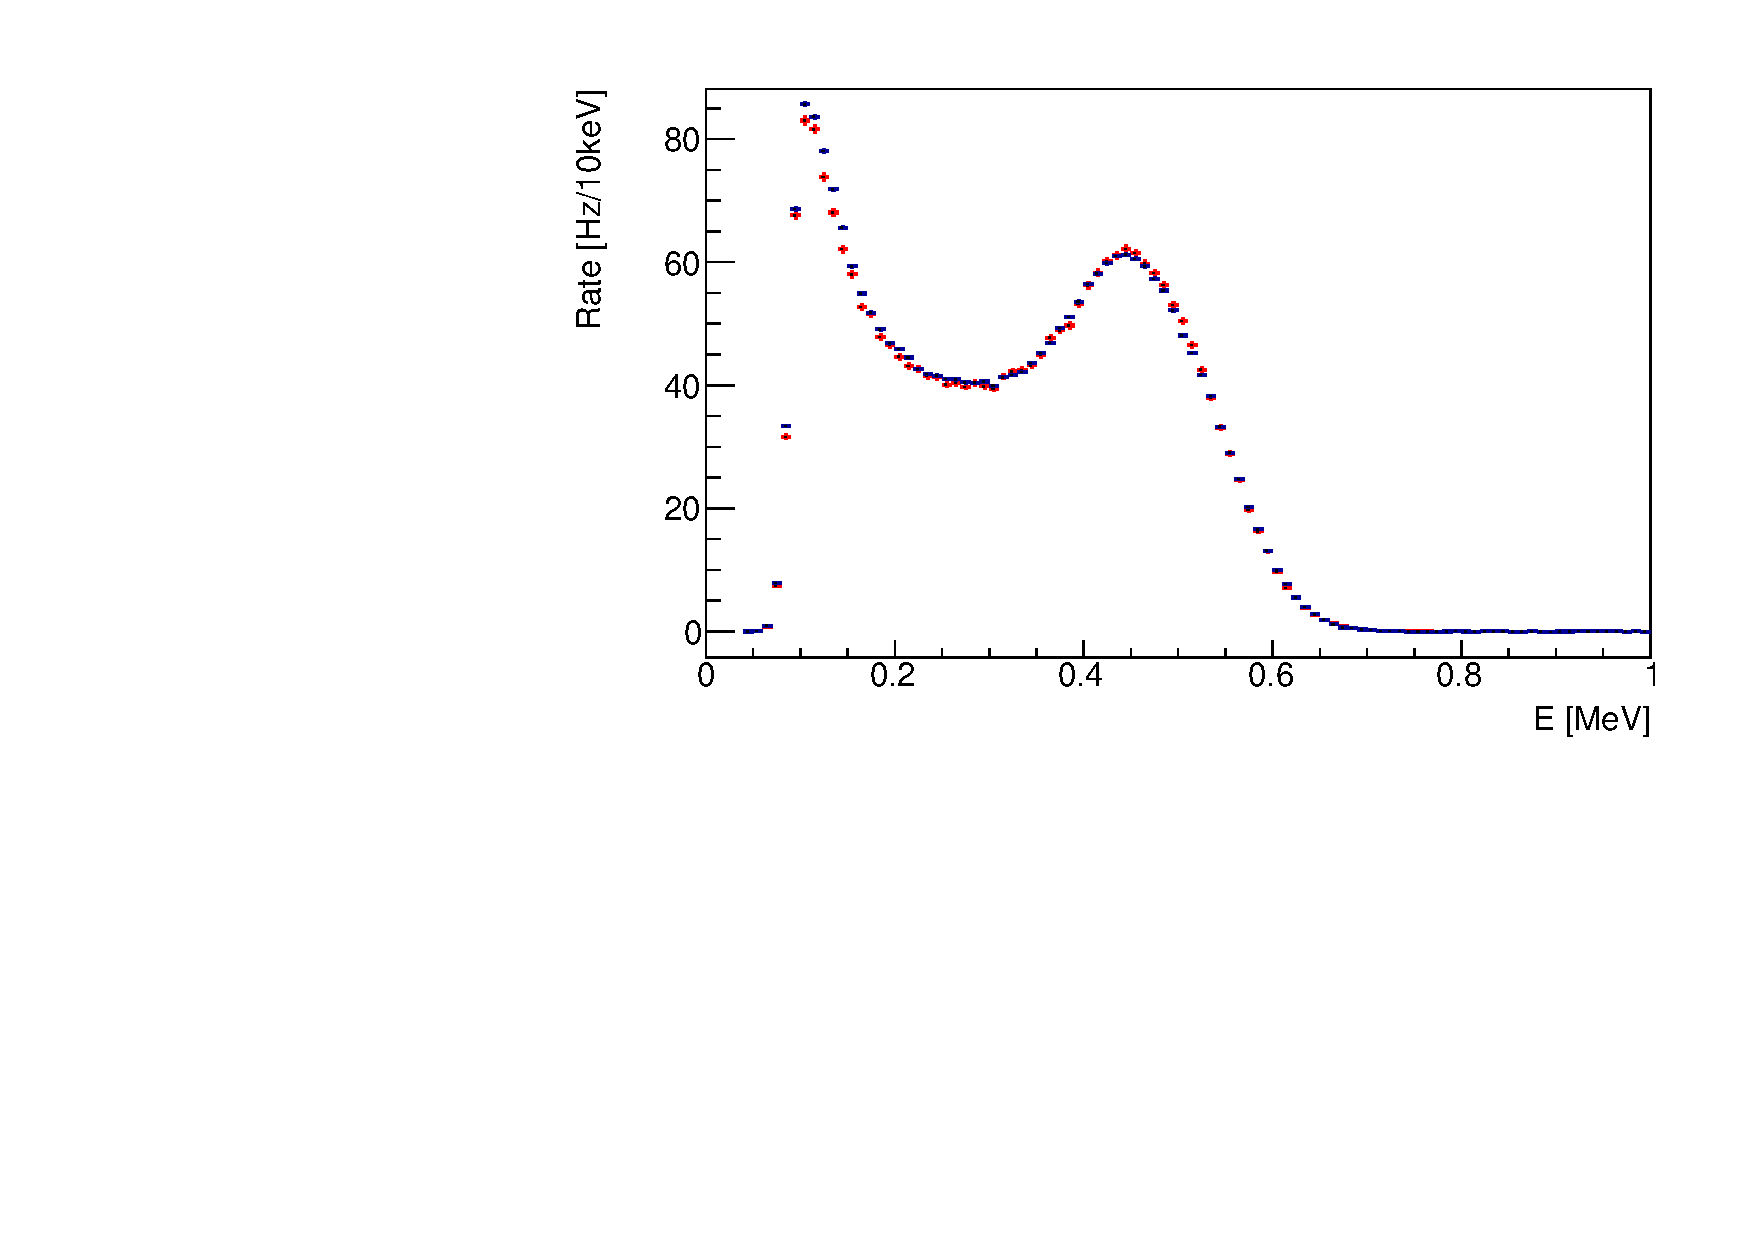
\includegraphics[width=60mm]{Figures/hCs137v2single.pdf}}\quad
\subfigure[]{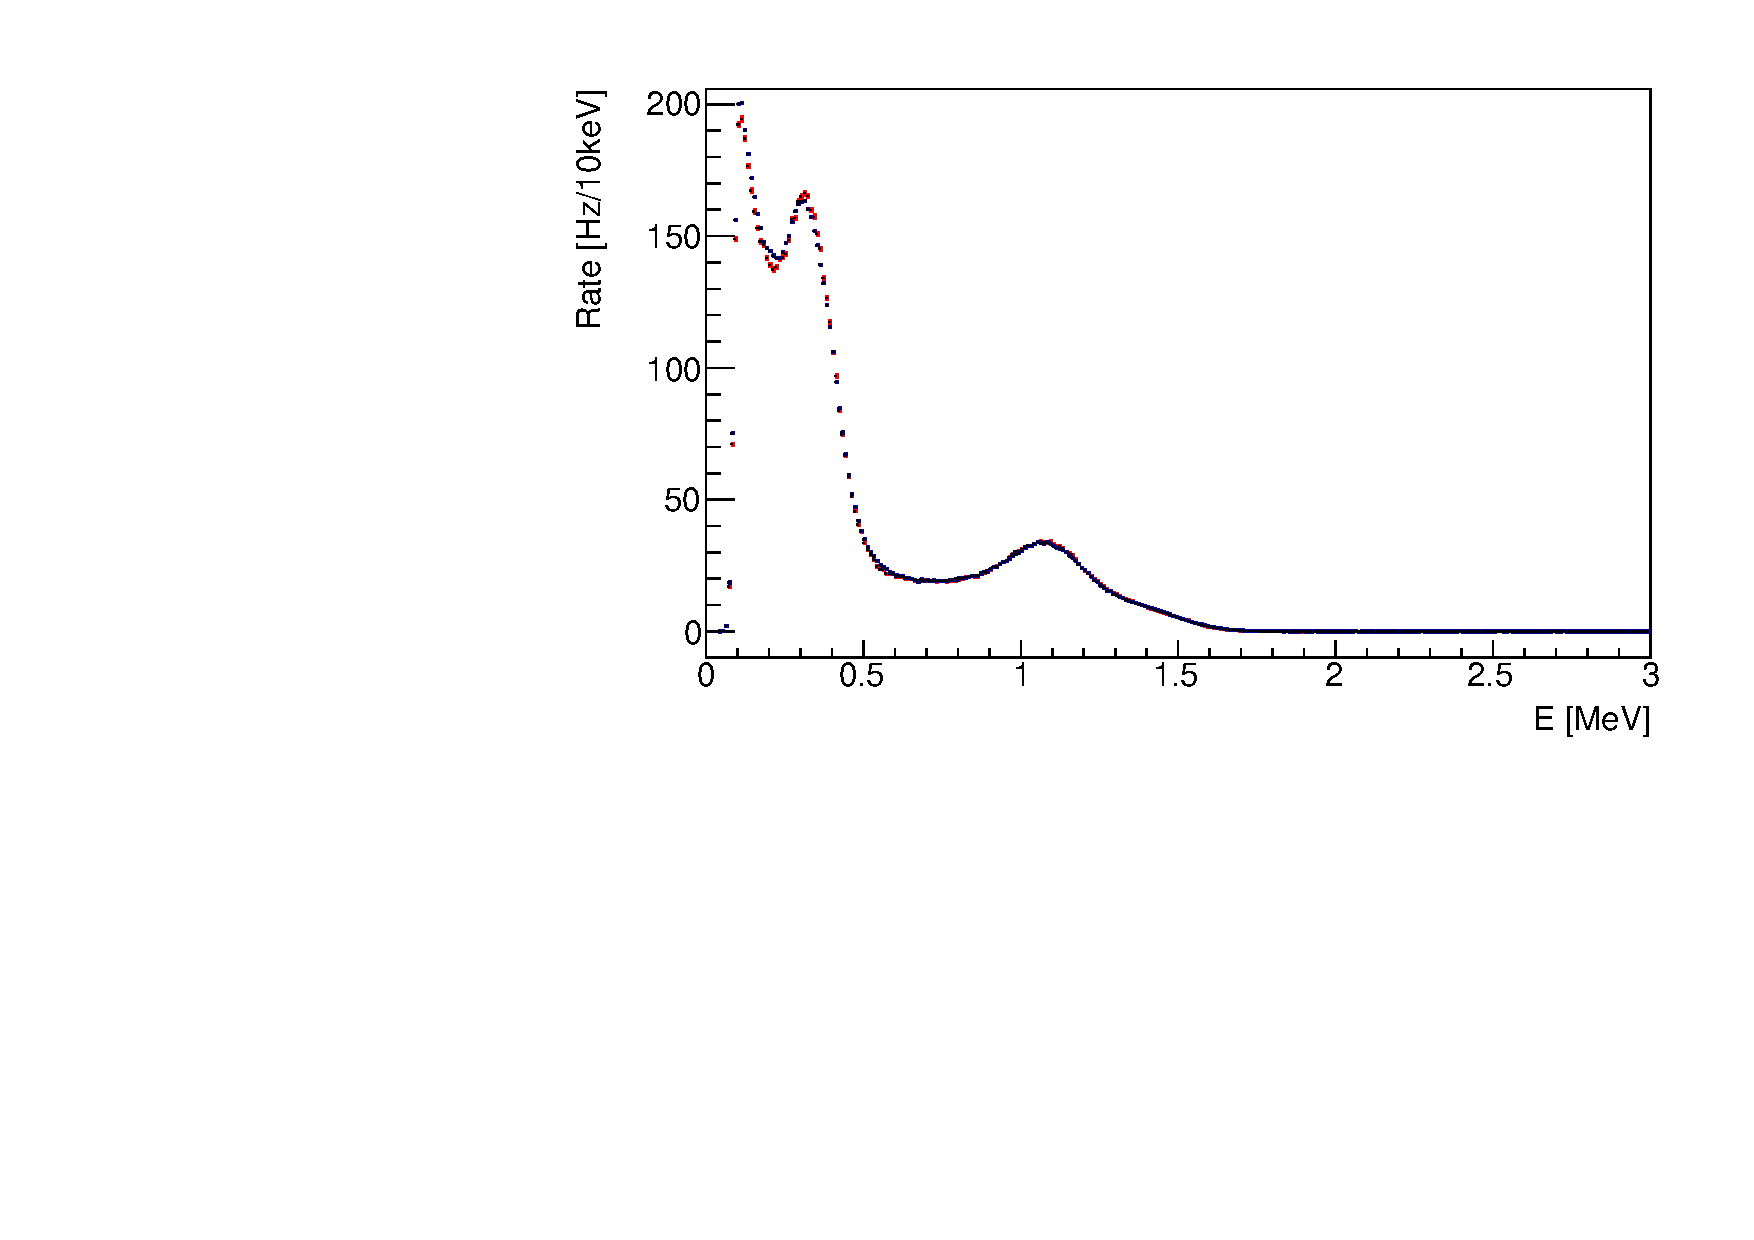
\includegraphics[width=60mm]{Figures/hNa22v2single.pdf}} \\
\subfigure[]{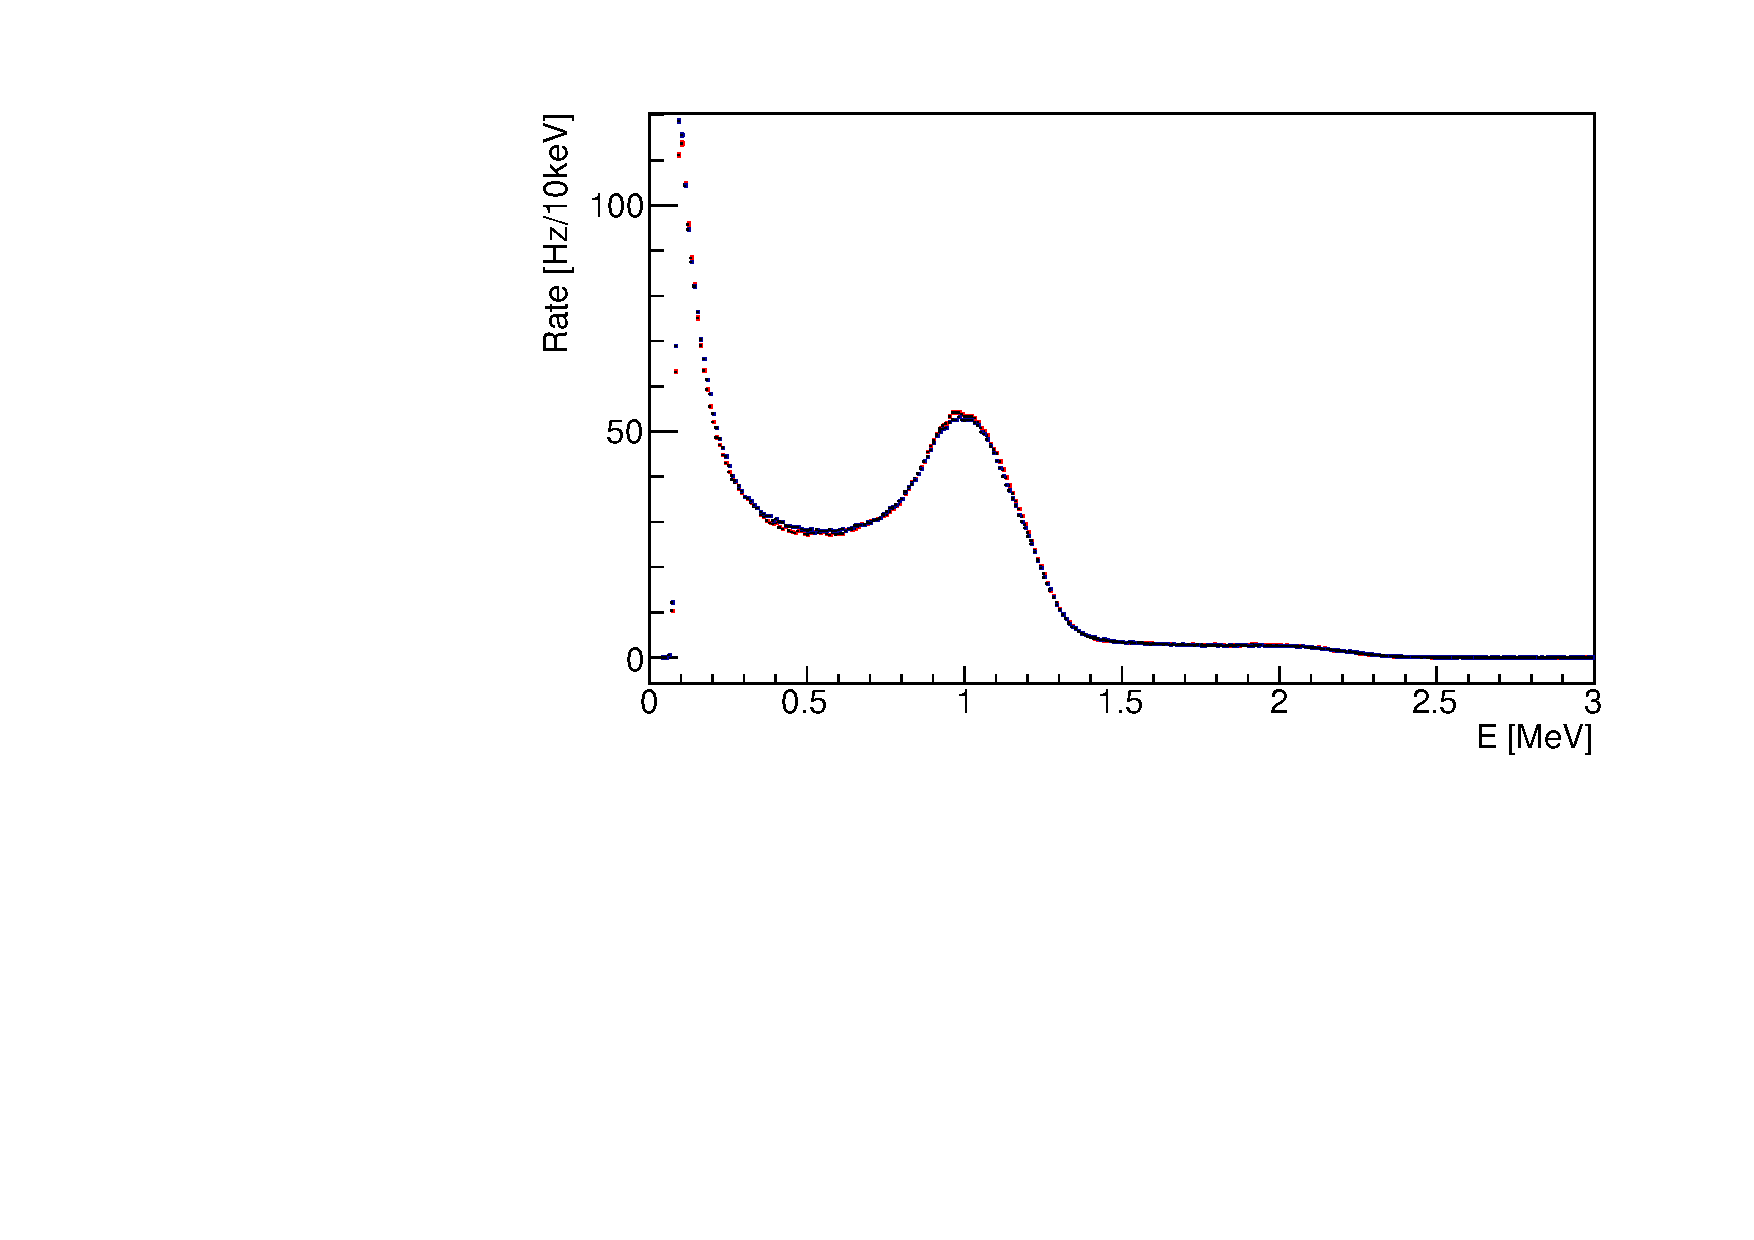
\includegraphics[width=60mm]{Figures/hCo60v2single.pdf}} \quad
\subfigure[]{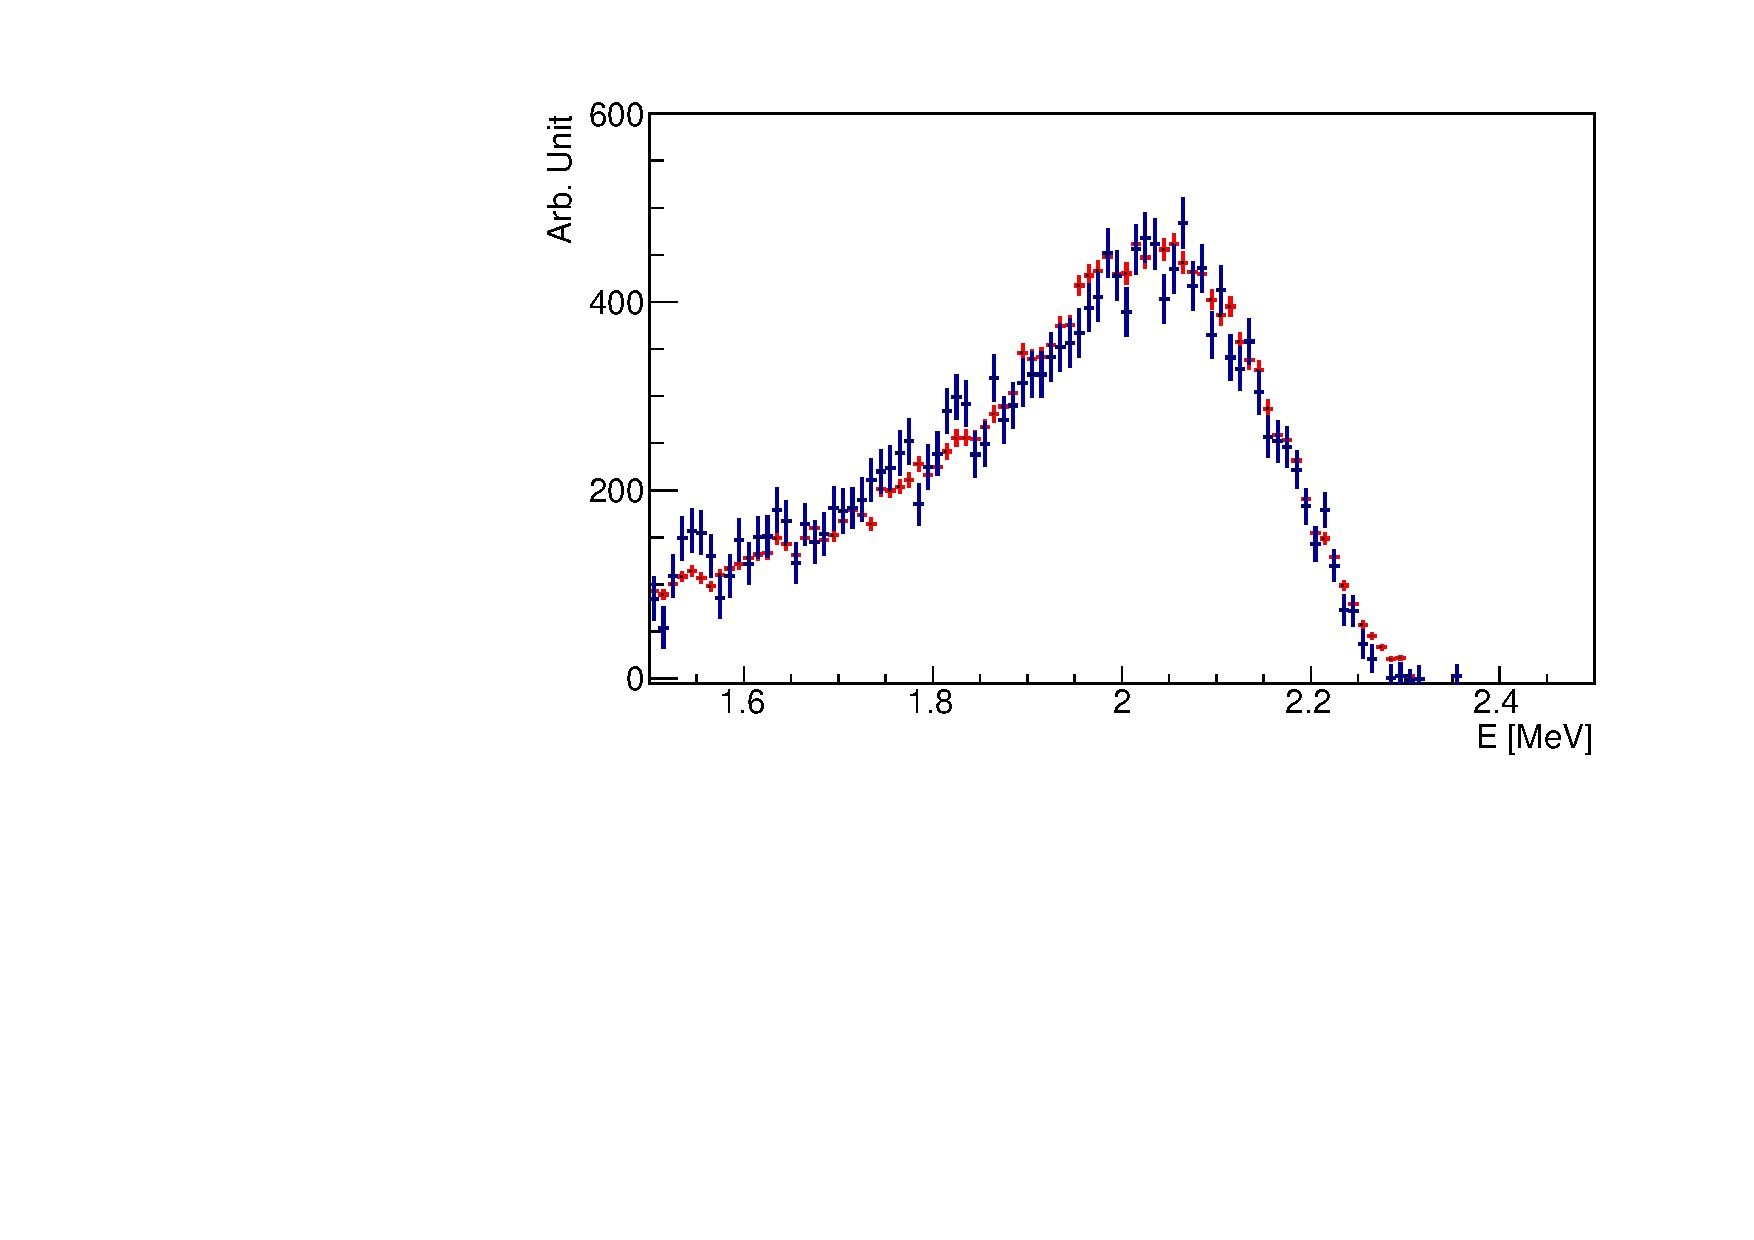
\includegraphics[width=60mm]{Figures/hCf252v2single.pdf}} \\
\subfigure[]{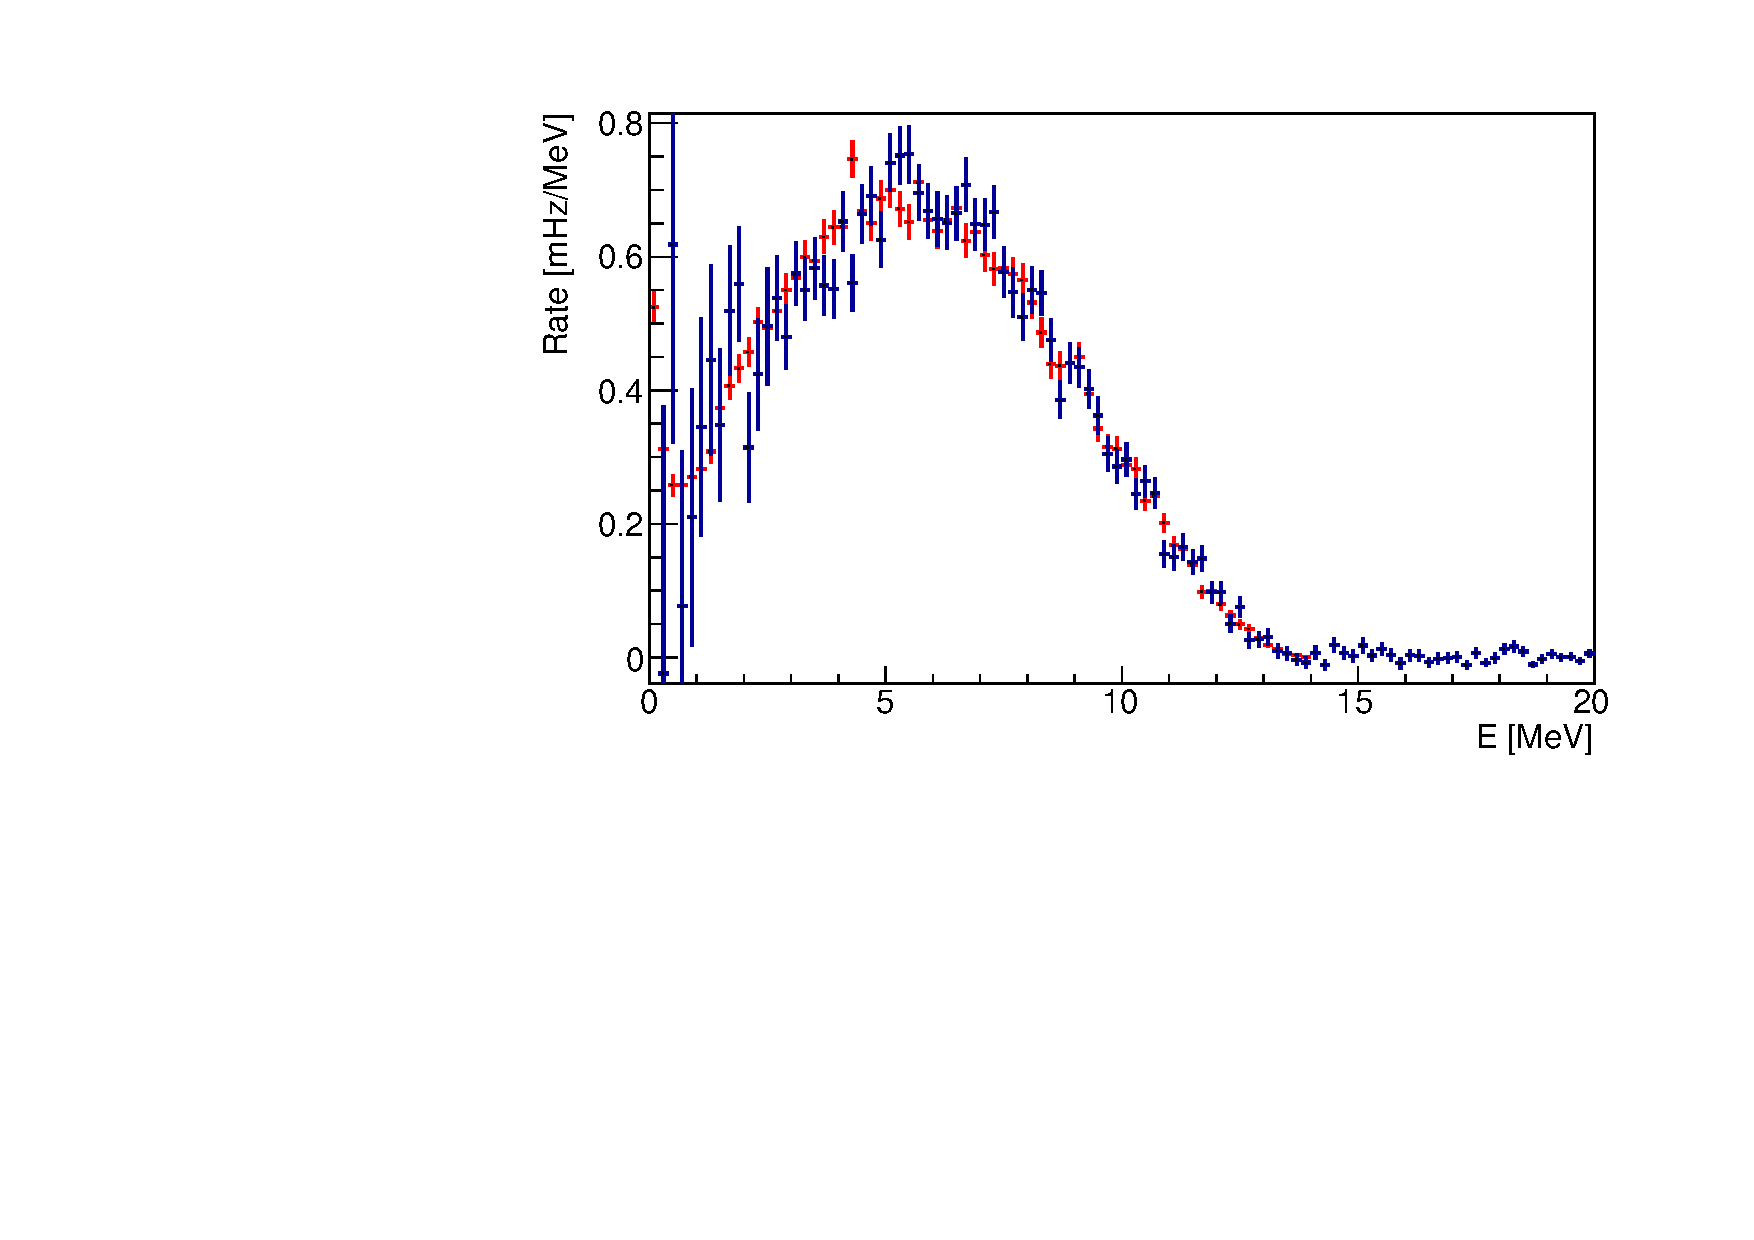
\includegraphics[width=60mm]{Figures/hB12v2single.pdf}} 
\caption[Single segment data to MC gamma energy comparisons]{The best fit results applied to single-segment data vs. MC comparison. (a) $^{137}$Cs, (b) $^{22}$Na, (c) $^{60}$Co, (d) $n$-H capture gamma from $^{252}$Cf, (e)$^{12}$B.}
\label{fig:goodfit}
\end{figure}
\newpage
\clearpage

\Subsection{Agreements Among Different Calibration Campaigns}
The energy scale model discussed in Subsection~\ref{sec:fulldet} was found with combined fitting of gamma calibrations taken in April 2018, neutron calibration performed in May 2018 and $^{12}$B for the first  neutrino spectrum analysis. 
Ideally, this model is expected to be compatible with other calibration campaigns with the same detector and calibration configurations within the energy scale uncertainty. 
Additional MC vs data comparisons were made by comparing calibration spectra and multiplicities of the August and December calibrations.
When the MC is compared to data, the nonlinearity parameters were fixed to the best fit values found with the April calibration. 
This is a powerful cross-check to ensure the best fit detector response model is able to find good agreement with data independent of time and detector configuration. 

The August calibration data was collected with calibration sources deployed at different locations inside the detector to maximize the number of functional segments close to the sources.
Similar to the April calibration campaign, the energy scale calibration is organized to deploy only one source in the detector for each calibration.
However, one gamma source was possibly left in the volume between the active detector and shielding, shown in Figure~\ref{fig:left}.
\begin{figure}[h!]
\centering
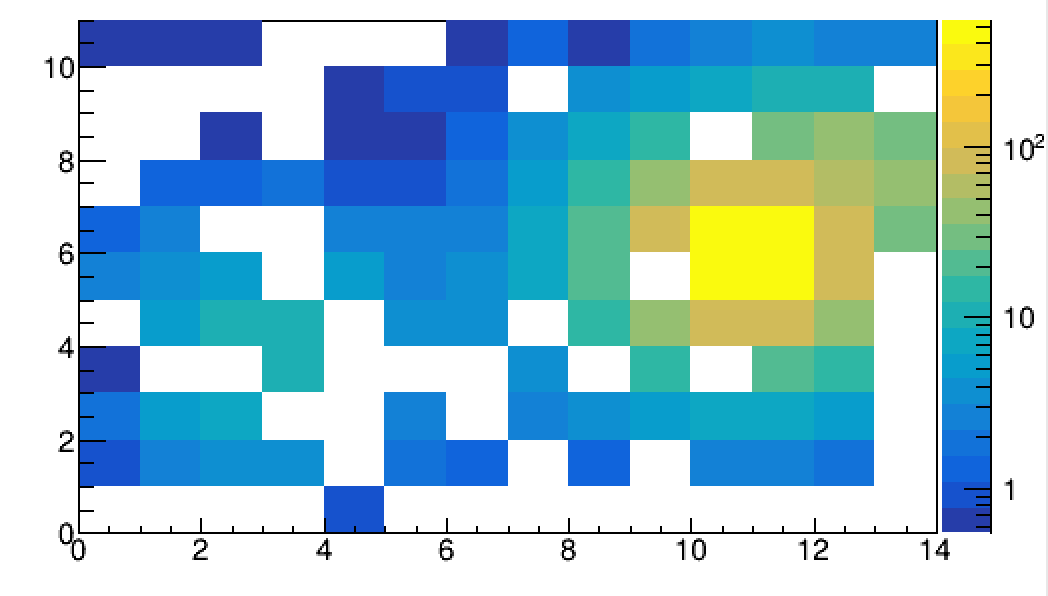
\includegraphics[width=100mm]{Figures/secondhotspot.png}
\caption[Indication of accidentally left calibration sources]{The event distribution of gamma event clusters, there is a secondary hot spot indicating another source trapped in the volume between detector volume and shielding.}
\label{fig:left}
\end{figure}
The contamination from the additional gamma source can cause an unknown spectrum to be added to the calibration energy spectrum.
With a sampling window for each hit of 400~ns, and the time interval between each hit within 20~ns, the overlapping of reconstructed energy from the additional calibration source is rare due the sources' radioactivity in 1~kBq scale.
Hence, the additional source can cause data and MC's disagreement in spectrum shape and multiplicity, but has minimum effect on the energy scale.

The December calibration campaign was organized with same goal as the April and August calibration, with the addition of the AmBe source described in the Section~\ref{sec:calibration}.
Although the $^{12}$B beta energy covers the range of 3 to 13.5~MeV, the AmBe 4.4~MeV single gamma is an additional powerful cross-check for PROSPECT to demonstrate its energy scale precision in the critical range where the IBD positron spectrum severely disagree with the Huber model.
The best fit AmBe MC and data is shown in Figure~\ref{fig:AmBeCompare}.

\begin{figure}[h!]
\centering
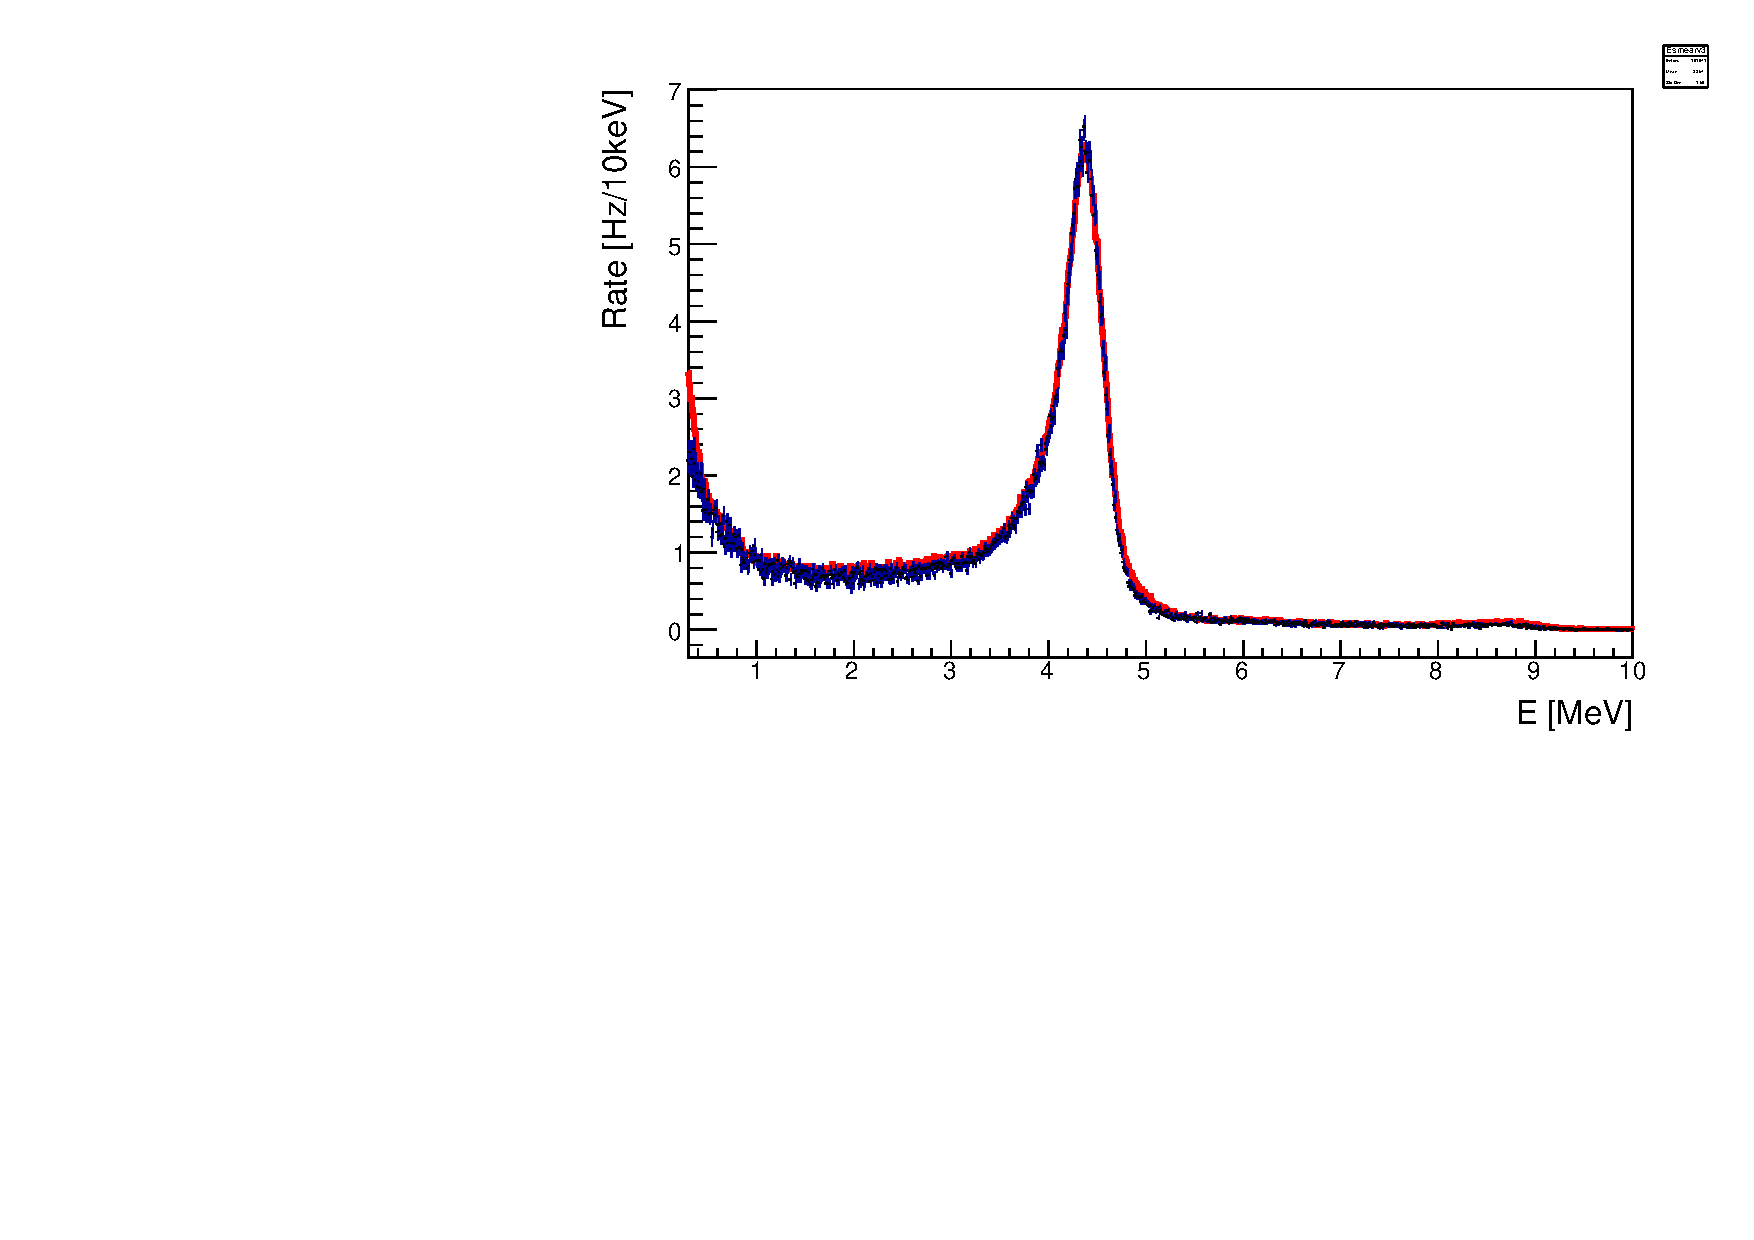
\includegraphics[width=80mm]{Figures/hAmBev2.pdf}
\caption[AmBe data to MC comparison]{AmBe reconstructed energy spectrum compared with the best fit MC.}
\label{fig:AmBeCompare}
\end{figure}
 
As a result of the cross-campaign check with the calibrations taken at different time in 2018, the ratio of reconstructed energy of the calibrations  and simulations is shown in Figure~\ref{fig:compare}.

\begin{figure}[h!]
\centering
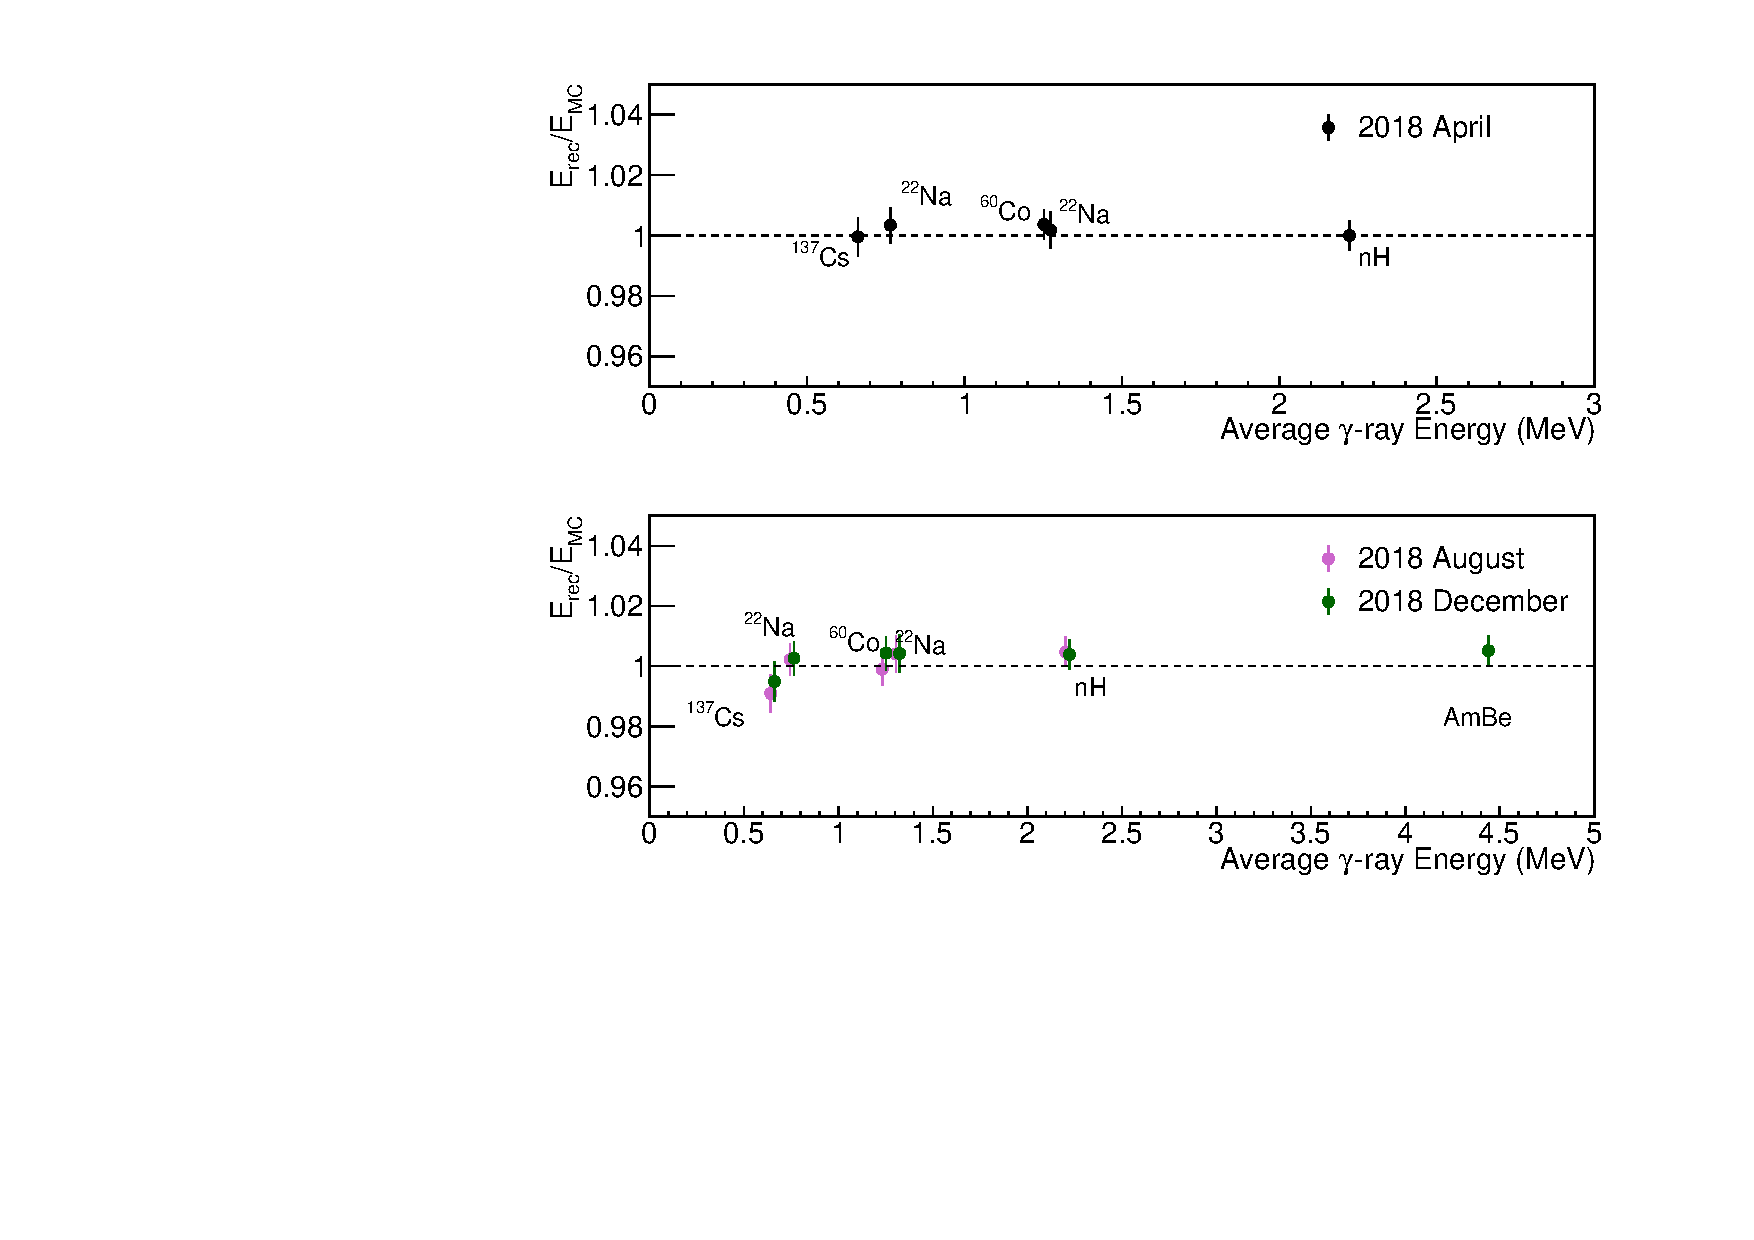
\includegraphics[width=0.8\textwidth]{Figures/PRDEscale3.pdf}
\caption[Discrepancies among calibration campaigns]{The discrepancy between April, August and December calibration energy scale is within $\sim0.6\%$ uncertainty.
	Data points of the August and December calibrations are intentionally shifted for clearer illustration.}
\label{fig:compare}
\end{figure}

An additional cross-check was made to characterize the reconstructed energy with respect to events with different multiplicities. 
Figure~\ref{fig:EvsMulti} shows the $E_{rec}/E_{mc}$ ratio of events with different multiplicities, in different calibrations in 2018.
Despite some of the multiplicity contains extremely small amount to events, the variation of energy scale in different calibration is roughly within 1\%.

\begin{figure}[h!]
\centering
\subfigure[]{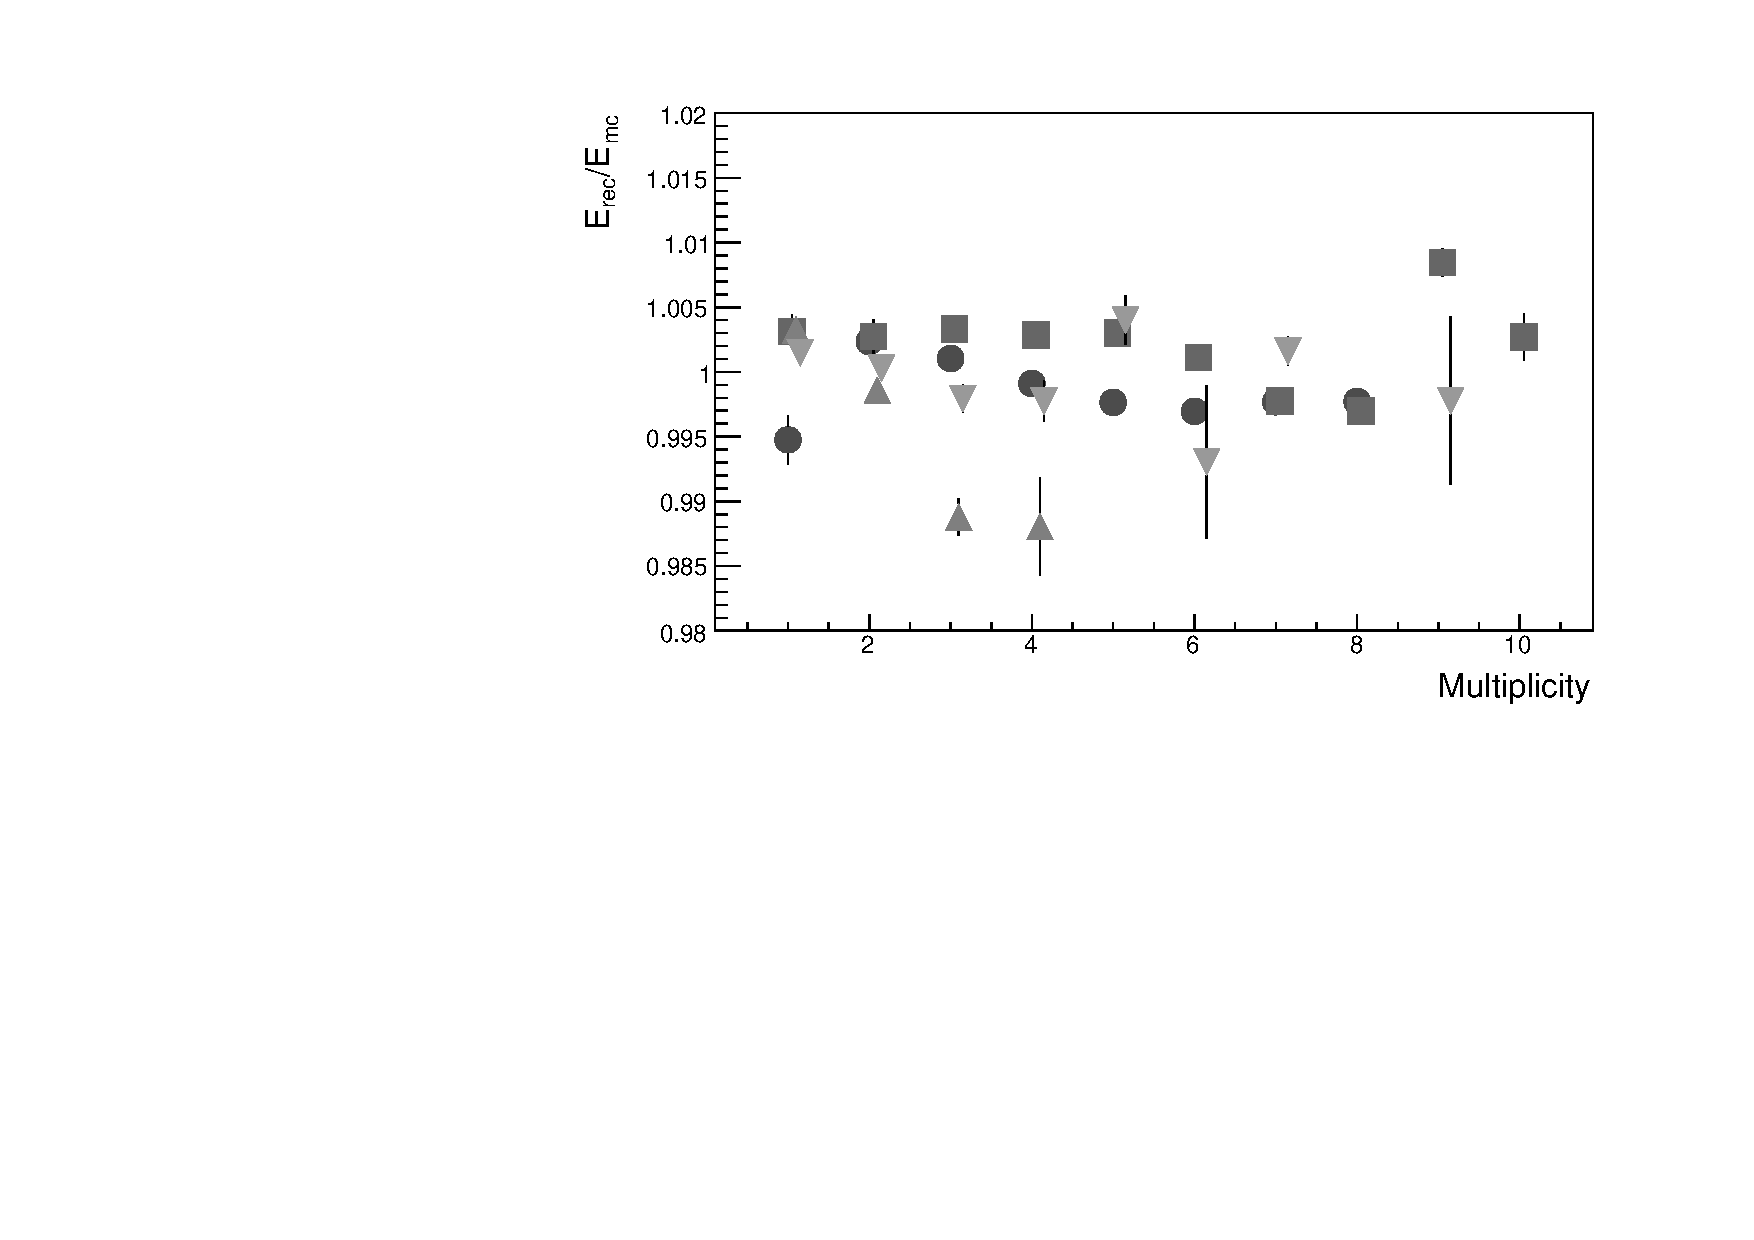
\includegraphics[width=60mm]{Figures/EvsMultiApr.pdf}}\quad
\subfigure[]{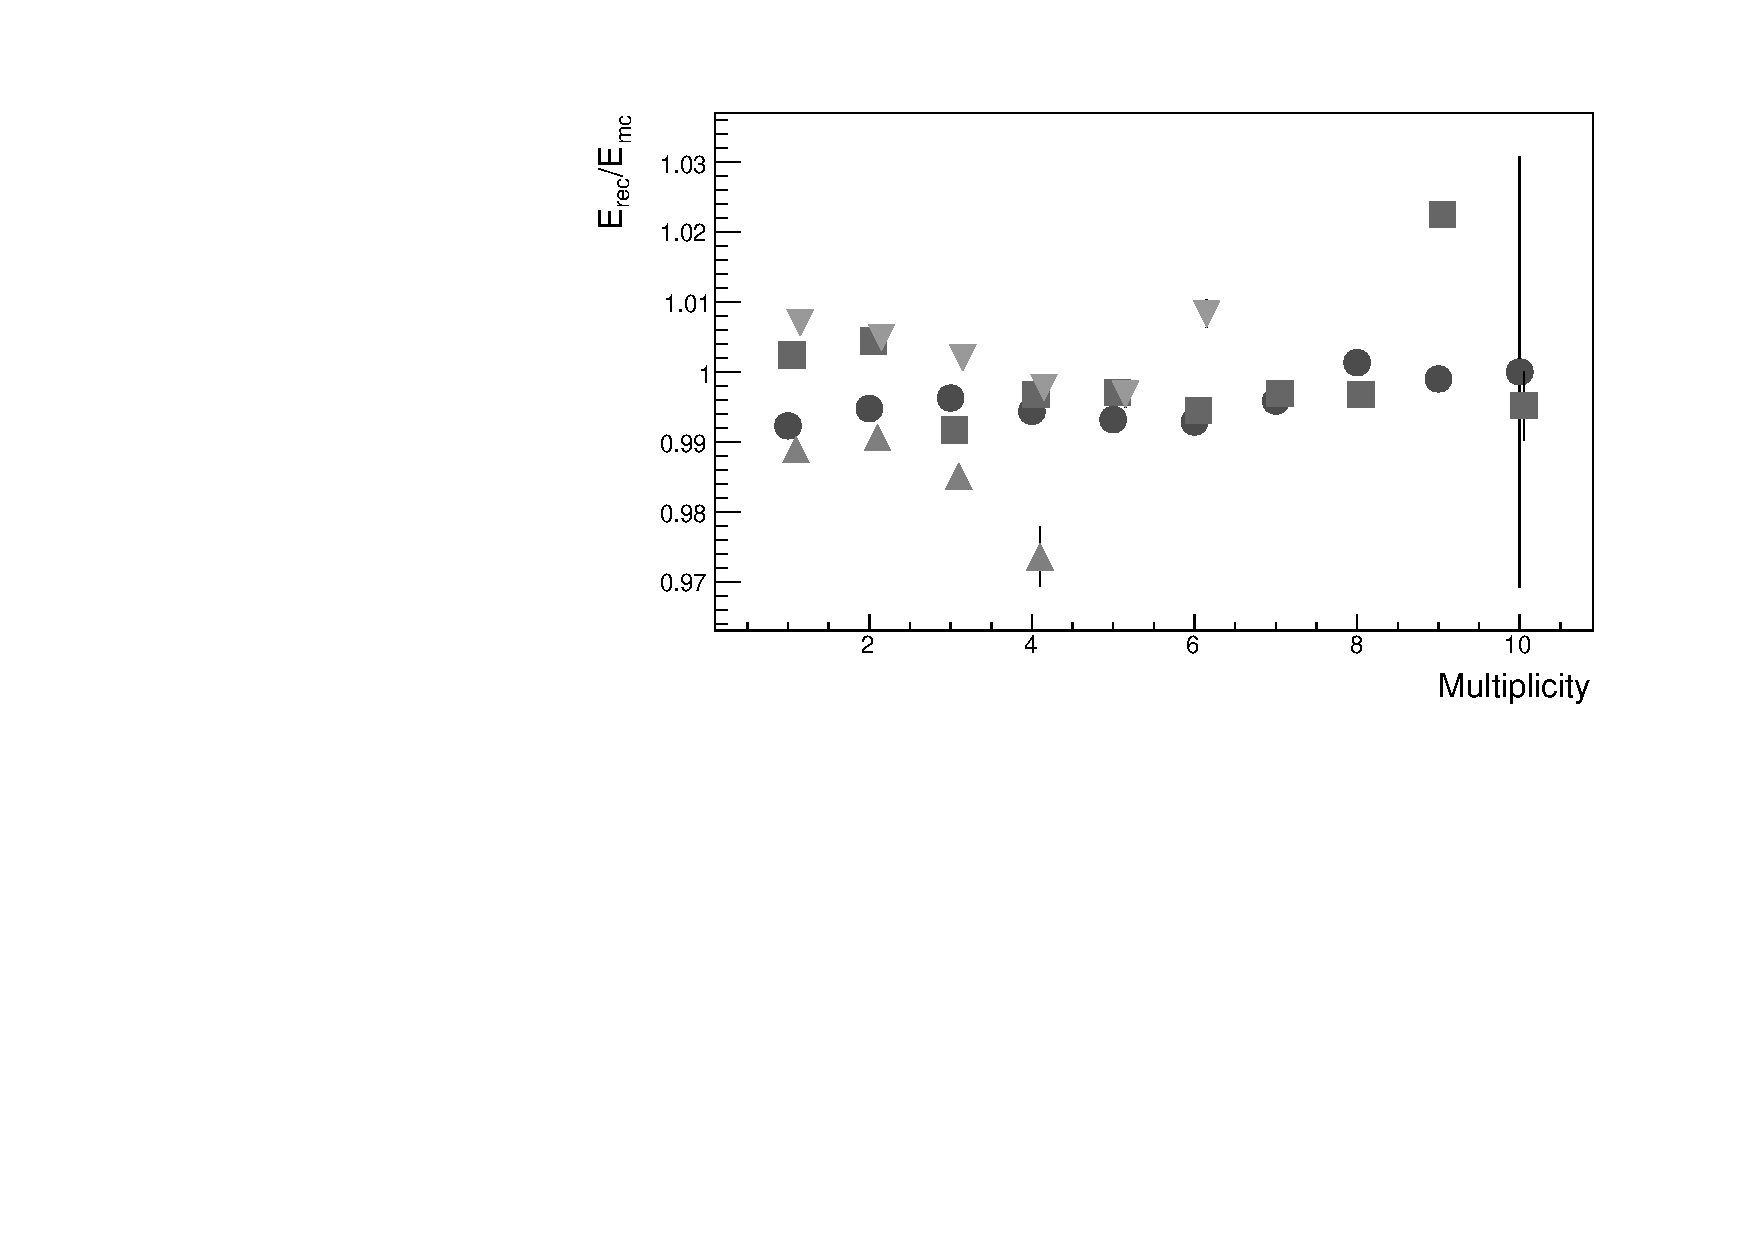
\includegraphics[width=60mm]{Figures/EvsMultiAug.pdf}} \\
\subfigure[]{\includegraphics[width=80mm]{Figures/EvsMultiDec2.pdf}} 
\caption[$E_{rec}/E_{mc}$ ratio vs. particle multiplicities]{$E_{rec}/E_{mc}$ ratio vs. particle multiplicities in different calibration campaigns in 2018. The statistical errors are shown in the figure. (a) April calibration, (b) August calibration, (c) December calibration.
}
\label{fig:EvsMulti}
\end{figure}

\Section{Position Dependence of Energy Response}

The energy response differs at different positions in the detector due to gamma energy leakage.
The leakage usually causes coherent downward shifts of the energy distribution.
To quantify the energy variation caused by gamma leakage, gamma sources were scanned through multiple PLA rods in the PROSPECT AD along the $z$-direction.
The $^{22}$Na sources were used to perform this calibration.
Event reconstructions of the gamma rays are performed in different volume sizes in the detector, as shown in Figure~\ref{fig:ring}.
The simulation of gamma leakage was tested by comparing MC simulation to the calibration data for each volume size case.
The comparisons include the $^{22}$Na source deployed at the center of detector, near the edge of detector along $z$ and near the corner of detector on the $x, y$ plane.
The simulated stopping power was also tested by comparing MC simulation to data with energy reconstruction in different sub-volumes of the detector.
The one-ring and three-rings volume cases are illustrated in Figure~\ref{fig:ring}.
\begin{figure}[h!]
\centering
\includegraphics[width=0.9\textwidth]{Figures/Ring.png}
\caption[Example of different volume sizes within three layers of segments.]{Example of different detector volume sizes within three layers (rings) of segments containing the calibration sources. In the case shown in this figure, the $^{22}$Na source is deployed near one edge of the PROSPECT AD.}
\label{fig:ring}
\end{figure}

Figure~\ref{fig:ringtests} shows the results of the different volume comparisons.
Sufficient agreement of the energy distributions were found between data and MC.
The data-MC differences of energy shift from center to edge are $8\pm1$~keV and $7\pm1$~keV for sources at detector center and corner, respectively.
Energy scales are also consistent within the energy scale uncertainty in 1-ring and 3-ring data-MC comparisons.
The data-MC difference of energy shifts of 1-ring and 3-ring reconstructions are $4\pm1$~keV and $5\pm1$~keV for sources at detector center and corner, respectively.
Therefore, a $\sim$8~keV energy shift offset is considered as the uncertainty in the IBD annihilation $\gamma$ leakage modelling
\begin{figure}[h!]
\centering
\includegraphics[width=0.9\textwidth]{Figures/Na22center.pdf}\\
\includegraphics[width=0.9\textwidth]{Figures/Na22_edge.pdf}
\caption[Reconstructed gamma energy of $^{22}$Na at different positions]{(Top) Distribution of total reconstructed gamma energy produced from $^{22}$Na sources deployed at the center of PLA rods.  
(Bottom) Distribution of total reconstructed gamma energy produced from $^{22}$Na sources deployed near one end of a PMT.  }
\label{fig:ringtests}
\end{figure}

\Section{Energy Scale Stability}

The energy scale stability is characterized by analyzing ambient neutron events, natural contaminant, and spiked $^{227}$Ac events.

\Subsection{BiPo Calibration}
The $\beta$ decay followed by the $\alpha$ decay from the Bi$\rightarrow$Po decay chain (BiPo) has a similar time coincidence as IBD events.
Alpha particles' small range, highly quenched light yield and high PSD values make their signals stable and easy to select in the PROSPECT AD. 
Thus,  BiPo decay events are used to test the stability of energy scale and resolution.
There are two major decay chains involving Bi$\rightarrow$Po$\rightarrow$Pb decays.
The dominant branch seen in the PROSPECT detector is BiPo from $^{222}$Rn, which is part of the $^{238}$U decay chain, a natural contaminant in most particle detectors. 
The $\beta$ and $\alpha$ are create as:
\begin{equation}
\ce{^{214}Bi -> ^{214}Po + e^- +  \nuebar}, \\
\ce{^{214}Po -> ^{210}Pb + \alpha}.
\end{equation}
The $^{214}$Bi decay generates $\beta$ particles with total energy of 3.275~MeV.
The kinetic energy of the $\alpha$ particle produced in $ \ce{^{214}Po}$ decay is 7.685~MeV in 99.99\% of decays.
The visible $\alpha$ energy $\sim$0.85~MeV.
The other BiPo decay is a part of the $^{232}$Th decay chain, also a natural contaminant of particle detectors. 
\begin{equation}
\ce{^{212}Bi -> ^{212}Po + e^- + \nuebar}, \\
\ce{^{212}Po -> ^{208}Pb + \alpha},
\end{equation}
where the total $\beta$ energy is 2.25~MeV with 9\% probability accompanying with de-excitation gamma ranging from 0.7~MeV to 1.8~MeV.
The $\alpha$ produced has 8.785~MeV kinetic energy and $\sim$1~MeV visible energy.  

The stability of the reconstructed $\alpha$ energy is the subject of the energy stability monitoring.

\Subsection{$^{227}$Ac Calibration}
The Rn-Po decay chain (RnPo) is a part of the decay chain of $^{227}$Ac uniformly spiked in the $^6$LiLS.
As shown in Figure~\ref{fig:RnPoChain}, the RnPo event consists of two coincident $\alpha$ decays of $^{219}$Rn and $^{215}$Po.
The $^{219}$Rn decays with Q-value = 6.95~MeV, and generates on $\alpha$ particle carrying the majority of the decay energy and a de-excitation $\gamma$ ray with 0.27~MeV (10.8\%) and 0.40~MeV (6.6\%).
The $^{215}$Po $\alpha$ decays produce monoenergetic 7.39~MeV $\alpha$ particle with 99.99\% probability.
\begin{figure}[h!]
\centering
\includegraphics[width=0.7\textwidth]{Figures/Ac227Chain.png}
\caption[The decay chain involving the decays from $^{227}$Ac to the RnPo events]{The decay chain involving the decays from $^{227}$Ac to the  RnPo events. }
\label{fig:RnPoChain}
\end{figure}

\Subsection{Other Stability Monitoring}
The $2.22$~MeV gamma ray of $n$-H capture events from the cosmogenic neutron background is also utilized as a long term monitor of energy scale stability.
The de-excitation gamma photons from $n$-H capture are selected based on time coincidence between proton recoils caused by fast cosmogenic neutron and the delayed gamma hits.
Another ubiquitous gamma source is an intrinsic contaminant of $^{208}$Tl uniformly distributed in the detector.
The $^{208}$Tl $\beta$ decay produces 2.61~MeV gammas with 99.75\% probability.
$^{208}$Tl gammas are selected with gamma-like PSD values with no coincident hits. 
Capture of reactor correlated neutrons in the experimental facilities also produces high-energy gammas.
The edge of the reactor correlated gamma spectrum is also monitored to test the detector energy scale stability.

\Subsection{Quantifying the Stability}
The $^{214}$Po, $^{212}$Po, and $^{215}$Po $\alpha$ energies, as well as the other single gamma energies are used  to monitor the energy scale stability. 
The energy scale stability for the 2018 reactor neutrino spectrum measurement is shown in the top panel of Figure~\ref{fig:StabilityTime}.
The energy scale variation is within $\pm$0.5\% through the full PROSPECT 2018 dataset.
The reactor-on and -off difference in energy scale is within $\pm$0.2\%.

\begin{figure}[h!]
\centering
\includegraphics[width=0.8\textwidth]{Figures/StabilityVsTime.pdf}
\caption[Detector stability characterization]{
(Top) The reconstructed energy scale stability characterized by the BiPo and RnPo $\alpha$ energy, the gamma energies from the multiple sources.
(Top-middle) The energy resolution stability. 
(Bottom-middle) The RMS of reconstructed $z$ positions calculated from $^{214}$Po, $^{212}$Po, and $^{215}$Po $\alpha$ decays.
(Bottom) The prompt and delayed $\Delta z$ of the RnPo $\alpha\alpha$ decay.}
\label{fig:StabilityTime}
\end{figure}

\Section{Energy Resolution Stability}

The energy resolution stability is characterized with the same calibration analysis as the energy scale stability study above.
The energy distribution of $^{214}$Po, $^{212}$Po, and $^{215}$Po $\alpha$ hits, and the single gamma events are fitted with Gaussian functions to quantify the standard deviation in each run. 
The stability of energy resolution is shown in the upper-middle panel of Figure~\ref{fig:StabilityTime}, indicating energy resolution stability within $\pm$5\% and variation between reactor-on and -off periods of $\pm$2\%.

\Section{Position Resolution Characterization }

Position reconstruction is vital in IBD selection, for the variation of $z$ position resolution can cause a change in IBD detection efficiency.
BiPo and RnPo events are utilized to characterize the stability of position reconstruction and position resolution.
Because the BiPo and RnPo events are uniformly distributed in the detector, the $z$ position distribution of various Po $\alpha$ particles can be used to monitor the consistency of $z$ position reconstruction.
Another advantage of the RnPo events is that their vertexes of prompt and delayed signals are approximately at the same position, while the mobility of the $\alpha$ particles in the PROSPECT AD is on the scale of \textmu m.
Thus, the distribution of prompt and delayed hit distances' $dz$ is used to quantify the position resolution along the segments.
The $z$ and $\Delta z$ distribution of produced $\alpha$ particles are shown in Figure~\ref{fig:ZReco}.
The $\Delta z$ distribution is fitted with Gaussian function to search for the best fit standard deviation.
The resolution of position reconstruction is 49.9$\pm$0.1~mm.
\begin{figure}[h!]
\centering
\includegraphics[width=0.95\textwidth]{Figures/PosDist.pdf}
\caption[Distributions of $z$ and $dz$ of Po decayed $\alpha$ ]{
(Left) The reconstructed $z$ distribution of Po produced $\alpha$ particles in a segment.
(Right) The distribution of $dz$ between prompt and delayed hits of RnPo $\alpha\alpha$.}
\label{fig:ZReco}
\end{figure}

The stability of reconstructed position and position resolution is shown in the bottom two panels in Figure~\ref{fig:StabilityTime}.
The variation of reconstructed position are quantified by comparison the RMS of the $z$ positions of $^{214}$Po, $^{212}$Po, and $^{215}$Po $\alpha$ hits.
The RMS values exhibit stability within $\pm$1.5\% along the 1176~mm long segments, which is equivalent to 2~cm variation.
The position resolution calculated with $\Delta z$ between two RnPo hits indicates 7\% (3.5~mm) variation.

\Section{Reconstruction Differences Among Segments}

Because of $\alpha$ particles' small range of movement, a RnPo decay's prompt and delay signals are in a single segment.
Hence, the spiked $^{227}$Ac is an ideal calibration source to measure the relative segment volume difference by counting the RnPo event rate in each segment.
The rate of RnPo events is shown in Figure~\ref{fig:RnPoRate}, exhibiting that RnPo rates in all segments vary within 2\%.
\begin{figure}[h!]
\centering
\includegraphics[width=0.7\textwidth]{Figures/RnPoRate.pdf}
\caption[RnPo rate per segment ]{
The rate of RnPo events in each segment.}
\label{fig:RnPoRate}
\end{figure}

The energy of the Po $\alpha$ decays, as well as the reconstructed gamma energy of $^{137}$Cs gamma calibration throughout the detector, are compared among all segments.
The reconstructed energy distribution of the Po $\alpha$ decays are fitted with a Gaussian function to search for the best mean energy.
The gamma energy of $^{137}$Cs detected by each individual segment was compared to a MC template energy spectrum to quantify the energy scale variation among all segments.
The variation of energy scale and resolution among segments are shown in Figure~\ref{fig:EvsSegment}.
All segments' reconstructed energies are uniform within $\pm$1\%.
Energy resolution of each segment varies within $\pm$5\%.
\begin{figure}[h!]
\centering
\includegraphics[width=0.7\textwidth]{Figures/EvsSegment.pdf}
\caption[Energy scale variation among segments]{
(Top) Energy scale variation among all segments.
(Bottom) Energy resolution variation among all segments.}
\label{fig:EvsSegment}
\end{figure}

\Section{Finalized Detector Response Model and Uncertainties for the IBD Spectrum Analysis}
\label{sec:escalefinal}

According to Section \ref{sec:dataMC}, the energy non-linearity model was finalized based on the  data vs MC comparison of the full detector reconstructed calibration gammas and neutrons.
The energy scale of the PROSPECT AD can be expressed as the ratio of true energy to reconstructed energy of average particles from different calibrations, $E_{rec}/E_{true}$, as shown in Figure \ref{fig:compare}.
This figure indicates that, at lower energy, the scale is able to vary $\sim0.6\%$ from 1.
This uncertainty is partially contributed by the energy scale fluctuation caused by the uncertainty the nonlinearity model.  Another contributor, a 0.46\% absolute uncertainty that is characterized with $^{12}$B data vs MC comparison discussed below.

Data vs MC comparison of the $^{12}$B energy spectrum was used to demonstrate the energy scale at higher energy, shown in Figure \ref{fig:B12final}. 
The fractional residual calculated between data and MC was fitted with a straight line whose slope is the energy scale difference between data and MC. 
The best fit slope in Figure \ref{fig:B12final} indicates that the energy scale of data and MC of the $^{12}$B beta spectrum differs by $0.33 \pm 0.46\%$.

\begin{figure}[h!]
\centering
\subfigure[]{\includegraphics[width=0.48\textwidth]{Figures/hB12v2.pdf}} \quad
\subfigure[]{\includegraphics[width=0.48\textwidth]{Figures/hB12residualv2.pdf}} \quad
\caption[Best fit MC compared to data of the $^{12}$B spectrum]{(a) Full detector MC-data comparison for the $^{12}$B spectrum. (b) The fractional residual of $^{12}$B data and MC spectrum. The average residual of this comparison indicates a $0.33 \pm 0.46\%$ energy scale difference between data and MC.}
\label{fig:B12final}
\end{figure}

\begin{figure}[h!]
\centering
\subfigure[]{\includegraphics[width=0.48\textwidth]{Figures/hNa22v2.pdf}} \quad
\subfigure[]{\includegraphics[width=0.48\textwidth]{Figures/hNa22residual.pdf}} \quad
\caption[The data to best fit MC comparison of the $^{22}$Na gamma events]{The data to MC comparison of the $^{22}$Na spectrum and residual of comparison. (a) Full detector data-MC comparison for $^{22}$Na calibration. (b) The residual of this comparison.}
\label{fig:Na22final}
\end{figure}

The data vs. MC comparison of the $^{22}$Na gamma spectrum is a good way to indicate the multi-particle event reconstruction capability of the PROSPECT AD, see Figure \ref{fig:Na22final}.
This comparison validates the PG4 model's successful energy reconstruction of the annihilation gammas.
The gamma calibration sources supplied sufficient amount of statistics, such that they contributed negligibly to the overall model uncertainties. 
The $0.46\%$ energy scale uncertainty and statistical uncertainty in the $^{12}$B spectrum smeared the $\chi^2$ distribution during the quenching model search, thus enlarging the uncertainty of the nonlinearity model. 
To be conservative, the 0.46\% energy scale uncertainty in $^{12}$B is treated as a systematic energy scale uncertainty.

The energy resolution in Figure \ref{fig:resolution} shows the resolution of each energy distribution of the calibrations, fitted with Function \ref{eql:resolution}.
The energy resolution at 1 MeV is 4.76\%$\pm$0.2\%.
This result also validates the Gaussian smearing of all events' energy with the resolution equivalent to 325~PE/MeV photostatistics (described in Section~\ref{sec:calibration}).

\begin{figure}[h!]
\centering
\includegraphics[width=80mm]{Figures/PRDResolution.pdf}
\caption[Energy resolution function fitting to the standard deviations of gamma calibration spectra]{The energy resolution characterized with mean energies of each calibration fitted with the resolution function. 
The errors include both statistical uncertainty and uncertainty of the nonlinearity model.}
\label{fig:resolution}
\end{figure}

The energy resolutions in the spectrum analysis are forced to be smeared to match the poorest resolution measured in detector during data taking.
The uncertainty of the energy resolutions is thus quantified with the uncertainty of the poorest measured photostatistics ($325\pm17$ PE/MeV).
This variation is consistent with the run-to-run energy resolution difference observed in the BiPo $\alpha$ energy resolution.

In conclusion, the uncertainty of energy response includes the following systematic uncertainties:
\begin{itemize}
    \item The $1-\sigma$ uncertainty of effective Birks$^\prime$ constants and effective Cherenkov efficiency, which are $k_{B1} = 0.132 \pm 0.004$ mm/MeV, $k_{B2} = 0.023 \pm 0.004$ mm/MeV, $k_C = 37 \pm 2\%$, $A = 100.26\pm0.46\%$.
    \item The 0.46\% uncertainty of absolute energy scale.
    \item The analysis ZLE threshold uncertainty of $90\pm5$ keV.
    \item The uncertainty of the artificial smearing $325\pm17$ PE/MeV.
    \item The uncertainty of the thickness of the optical separators of $1.18\pm0.05$ mm.
\end{itemize}
Each of the uncertainties above are turned into a covariance matrix individually. 
As a result, the covariance matrices from energy scale uncertainty and thickness uncertainty of separators are shown in Figure \ref{fig:cov}.

\begin{figure}[h!]
\centering
\subfigure[]{\includegraphics[width=0.48\textwidth]{Figures/nonlinearcov.pdf}} \quad
\subfigure[]{\includegraphics[width=0.48\textwidth]{Figures/thickcov.pdf}} \quad
\caption[Reduced covariance matrices]{The reduced covariance matrices used for PROSPECT's IBD spectrum analysis. (a) IBD covariance matrix for the uncertainty in the nonlinearity and energy scale model.
(b) IBD covariance matrix for the uncertainty of panel thickness.}
\label{fig:cov}
\end{figure}

For the IBD spectrum measurement, the finalized calibration to simulation comparisons are shown in Figure~\ref{fig:calibfinal}.
The April gamma calibrations, the $n$-H capture gamma, and the $^{12}$B beta energy are compared to the data with the uncertainties listed above.
The errors of the $E_{rec}/E_{mc}$ ratio in Figure~\ref{fig:compare} also contain those uncertainties.
\begin{figure}[h!]
\centering
\includegraphics[width=0.7\textwidth]{Figures/CalibPaperPlotV2.pdf}
\caption[Calibration data to best fit MC comparison with energy scale uncertainties.]{Calibration data to best fit MC comparison with energy scale uncertainties. 
(Top) The E$_{rec}$ for detector-center $\gamma$-ray source deployments; (Center top) The E$_{rec}$ for $n$-H captures from a detector-center $^{252}$Cf source deployment; (Center bottom) The E$_{rec}$ for cosmogenically-produced $^{12}$B; (Bottom) The event multiplicity for detector-center $^{137}$Cs and $^{22}$Na source deployments.  
Error bands indicate statistical (data) and systematic (PG4) uncertainties.}
\label{fig:calibfinal}
\end{figure}

The finalized detector response model is processed in the spectrum analysis in the form of a detector response matrix shown in the left plot of Figure~\ref{fig:responsematrix}.
This matrix translates neutrino energy to the reconstructed IBD prompt energy.
The default range of the input neutrino (IBD prompt) energy is from 1.8 to 10~MeV (from 0 to 10~MeV) with bin width of 0.05~MeV.
After finalized energy model parameters are implemented in PG4, IBD events are simulated with equivalent neutrino energy uniformly distributed in each bin. 
The IBD event and neutron momentum distribution is simulated with respect to the HFIR core's relative location to the PROSPECT AD.
With two million IBD events simulated per bin, the energy response of the IBD events in each energy bin can provide sufficient statistical translation from neutrino energy to reconstructed IBD prompt energy.
The modeled energy spectrum of a single-energy neutrino MC dataset is shown in the right plot of the Figure~\ref{fig:responsematrix}.
The inconsistency of a naively smeared and Gaussian fitted prompt energy and the PROSPECT reconstruction is caused by
\begin{itemize}
	\item Energy loss in dead volumes of the PROSPECT AD.
	\item The 90~keV analysis ZLE threshold excludes low energy hits from a portion of clusters, reducing their total energy and widening and lowering the total energy distribution.
	\item The electron-positron annihilation gamma energy leakage, as well as the missing positron energy in dead segments, cause a significant amount of the prompt events with only one 511~keV energy deposition.
	\item The energy response nonlinearity.
\end{itemize} 
Being able to predict the detector response including unavoidable energy loss and resolution smearing, this detector response matrix is able to provide trustworthy conversion between neutrino energy and reconstructed IBD energy spectrum.
\begin{figure}[h!]
\centering
\includegraphics[width=0.48\textwidth]{Figures/FullResponse.pdf}
\includegraphics[width=0.48\textwidth]{Figures/MonoResponse.pdf}
\caption[Detector response matrix]{(Left) The detector response matrix for the conversions from neutrino spectrum models to PROSPECT's expected IBD prompt energy spectrum.
(Right) The IBD prompt energy spectrum generated from a 4.0~MeV antineutrino simulated through PG4. 
The red line represents a $\sim$3.2~MeV prompt energy with Gauss function smearing equivalent to 5.5\% energy resolution.
The gray dashed line is the smeared prompt energy shifted to match the PROSPECT reconstructed mean energy.}
\label{fig:responsematrix}
\end{figure}

